%&preformat-disser
\RequirePackage[l2tabu,orthodox]{nag} % Раскомментировав, можно в логе получать рекомендации относительно правильного использования пакетов и предупреждения об устаревших и нерекомендуемых пакетах
% Формат А4, 14pt (ГОСТ Р 7.0.11-2011, 5.3.6)
\documentclass[a4paper,14pt,oneside,openany]{memoir}

\input{common/setup}            % общие настройки шаблона
\input{common/packages}         % Пакеты общие для диссертации и автореферата
\synopsisfalse                      % Этот документ --- не автореферат
\input{Dissertation/dispackages}    % Пакеты для диссертации
\input{Dissertation/userpackages}   % Пакеты для специфических пользовательских задач

\input{Dissertation/setup}      % Упрощённые настройки шаблона

\input{common/newnames}         % Новые переменные, для всего проекта

%%% Основные сведения %%%
\newcommand{\thesisAuthorLastName}{\fixme{Кузнецов}}
\newcommand{\thesisAuthorOtherNames}{\fixme{Алексей Александрович}}
\newcommand{\thesisAuthorInitials}{\fixme{А.\,А.}}
\newcommand{\thesisAuthor}             % Диссертация, ФИО автора
{%
    \texorpdfstring{% \texorpdfstring takes two arguments and uses the first for (La)TeX and the second for pdf
        \thesisAuthorLastName~\thesisAuthorOtherNames% так будет отображаться на титульном листе или в тексте, где будет использоваться переменная
    }{%
        \thesisAuthorLastName, \thesisAuthorOtherNames% эта запись для свойств pdf-файла. В таком виде, если pdf будет обработан программами для сбора библиографических сведений, будет правильно представлена фамилия.
    }
}
\newcommand{\thesisAuthorShort}        % Диссертация, ФИО автора инициалами
{\thesisAuthorInitials~\thesisAuthorLastName}
%\newcommand{\thesisUdk}                % Диссертация, УДК
%{\fixme{xxx.xxx}}
\newcommand{\thesisTitle}              % Диссертация, название
{\fixme{Квазилинейная динамика вейбелевской турбулентности магнитного поля в анизотропной бесстолкновительной плазме  с различными функциями распределения частиц
}}
\newcommand{\thesisSpecialtyNumber}    % Диссертация, специальность, номер
{\fixme{XX.XX.XX}}
\newcommand{\thesisSpecialtyTitle}     % Диссертация, специальность, название (название взято с сайта ВАК для примера)
{\fixme{Физика плазмы}}
%% \newcommand{\thesisSpecialtyTwoNumber} % Диссертация, вторая специальность, номер
%% {\fixme{XX.XX.XX}}
%% \newcommand{\thesisSpecialtyTwoTitle}  % Диссертация, вторая специальность, название
%% {\fixme{Теория и~методика физического воспитания, спортивной тренировки,
%% оздоровительной и~адаптивной физической культуры}}
\newcommand{\thesisDegree}             % Диссертация, ученая степень
{\fixme{кандидата физико-математических наук}}
\newcommand{\thesisDegreeShort}        % Диссертация, ученая степень, краткая запись
{\fixme{канд. физ.-мат. наук}}
\newcommand{\thesisCity}               % Диссертация, город написания диссертации
{\fixme{Нижний Новгород}}
\newcommand{\thesisYear}               % Диссертация, год написания диссертации
{\the\year}
\newcommand{\thesisOrganization}       % Диссертация, организация
{\fixme{Федеральное государственное бюджетное научное учреждение «Федеральный исследовательский центр Институт прикладной физики им. А.В. Гапонова-Грехова Российской академии наук»}}
\newcommand{\thesisOrganizationShort}  % Диссертация, краткое название организации для доклада
{\fixme{ИПФ РАН}}

\newcommand{\thesisInOrganization}     % Диссертация, организация в предложном падеже: Работа выполнена в ...
{\fixme{Федеральном государственном бюджетном научном учреждении «Федеральный исследовательский центр Институт прикладной физики им. А.В. Гапонова-Грехова Российской академии наук»}}

%% \newcommand{\supervisorDead}{}           % Рисовать рамку вокруг фамилии
\newcommand{\supervisorFio}              % Научный руководитель, ФИО
{\fixme{Кочаровский Владимир Владиленович}}
\newcommand{\supervisorRegalia}          % Научный руководитель, регалии
{\fixme{Доктор физико-математических наук, академик РАН}}
\newcommand{\supervisorFioShort}         % Научный руководитель, ФИО
{\fixme{В.\,В.~Кочаровский}}
\newcommand{\supervisorRegaliaShort}     % Научный руководитель, регалии
{\fixme{д. ф.-м. н, академик РАН}}

%% \newcommand{\supervisorTwoDead}{}        % Рисовать рамку вокруг фамилии
%% \newcommand{\supervisorTwoFio}           % Второй научный руководитель, ФИО
%% {\fixme{Фамилия Имя Отчество}}
%% \newcommand{\supervisorTwoRegalia}       % Второй научный руководитель, регалии
%% {\fixme{уч. степень, уч. звание}}
%% \newcommand{\supervisorTwoFioShort}      % Второй научный руководитель, ФИО
%% {\fixme{И.\,О.~Фамилия}}
%% \newcommand{\supervisorTwoRegaliaShort}  % Второй научный руководитель, регалии
%% {\fixme{уч.~ст.,~уч.~зв.}}

\newcommand{\opponentOneFio}           % Оппонент 1, ФИО
{\fixme{Фамилия Имя Отчество}}
\newcommand{\opponentOneRegalia}       % Оппонент 1, регалии
{\fixme{доктор физико-математических наук, профессор}}
\newcommand{\opponentOneJobPlace}      % Оппонент 1, место работы
{\fixme{Не очень длинное название для места работы}}
\newcommand{\opponentOneJobPost}       % Оппонент 1, должность
{\fixme{старший научный сотрудник}}

\newcommand{\opponentTwoFio}           % Оппонент 2, ФИО
{\fixme{Фамилия Имя Отчество}}
\newcommand{\opponentTwoRegalia}       % Оппонент 2, регалии
{\fixme{кандидат физико-математических наук}}
\newcommand{\opponentTwoJobPlace}      % Оппонент 2, место работы
{\fixme{Основное место работы c длинным длинным длинным длинным названием}}
\newcommand{\opponentTwoJobPost}       % Оппонент 2, должность
{\fixme{старший научный сотрудник}}

%% \newcommand{\opponentThreeFio}         % Оппонент 3, ФИО
%% {\fixme{Фамилия Имя Отчество}}
%% \newcommand{\opponentThreeRegalia}     % Оппонент 3, регалии
%% {\fixme{кандидат физико-математических наук}}
%% \newcommand{\opponentThreeJobPlace}    % Оппонент 3, место работы
%% {\fixme{Основное место работы c длинным длинным длинным длинным названием}}
%% \newcommand{\opponentThreeJobPost}     % Оппонент 3, должность
%% {\fixme{старший научный сотрудник}}

\newcommand{\leadingOrganizationTitle} % Ведущая организация, дополнительные строки. Удалить, чтобы не отображать в автореферате
{\fixme{Федеральное государственное бюджетное образовательное учреждение высшего
профессионального образования с~длинным длинным длинным длинным названием}}

\newcommand{\defenseDate}              % Защита, дата
{\fixme{DD mmmmmmmm YYYY~г.~в~XX часов}}
\newcommand{\defenseCouncilNumber}     % Защита, номер диссертационного совета
{\fixme{Д\,123.456.78}}
\newcommand{\defenseCouncilTitle}      % Защита, учреждение диссертационного совета
{\fixme{Название учреждения}}
\newcommand{\defenseCouncilAddress}    % Защита, адрес учреждение диссертационного совета
{\fixme{Адрес}}
\newcommand{\defenseCouncilPhone}      % Телефон для справок
{\fixme{+7~(0000)~00-00-00}}

\newcommand{\defenseSecretaryFio}      % Секретарь диссертационного совета, ФИО
{\fixme{Фамилия Имя Отчество}}
\newcommand{\defenseSecretaryRegalia}  % Секретарь диссертационного совета, регалии
{\fixme{д-р~физ.-мат. наук}}            % Для сокращений есть ГОСТы, например: ГОСТ Р 7.0.12-2011 + http://base.garant.ru/179724/#block_30000

\newcommand{\synopsisLibrary}          % Автореферат, название библиотеки
{\fixme{Название библиотеки}}
\newcommand{\synopsisDate}             % Автореферат, дата рассылки
{\fixme{DD mmmmmmmm}\the\year~года}

% To avoid conflict with beamer class use \providecommand
\providecommand{\keywords}%            % Ключевые слова для метаданных PDF диссертации и автореферата
{}
             % Основные сведения
\input{common/fonts}            % Определение шрифтов (частичное)
\input{common/styles}           % Стили общие для диссертации и автореферата
\input{Dissertation/disstyles}  % Стили для диссертации
\input{Dissertation/userstyles} % Стили для специфических пользовательских задач

%%% Библиография. Выбор движка для реализации %%%
% Здесь только проверка установленного ключа. Сама настройка выбора движка
% размещена в common/setup.tex
\ifnumequal{\value{bibliosel}}{0}{%
    \input{biblio/predefined}   % Встроенная реализация с загрузкой файла через движок bibtex8
}{
    \input{biblio/biblatex}     % Реализация пакетом biblatex через движок biber
}

% Вывести информацию о выбранных опциях в лог сборки
\typeout{Selected options:}
\typeout{Draft mode: \arabic{draft}}
\typeout{Font: \arabic{fontfamily}}
\typeout{AltFont: \arabic{usealtfont}}
\typeout{Bibliography backend: \arabic{bibliosel}}
\typeout{Precompile images: \arabic{imgprecompile}}
% Вывести информацию о версиях используемых библиотек в лог сборки
\listfiles

%%% Управление компиляцией отдельных частей диссертации %%%
% Необходимо сначала иметь полностью скомпилированный документ, чтобы все
% промежуточные файлы были в наличии
% Затем, для вывода отдельных частей можно воспользоваться командой \includeonly
% Ниже примеры использования команды:
%
%\includeonly{Dissertation/part2}
%\includeonly{Dissertation/contents,Dissertation/appendix,Dissertation/conclusion}
%
% Если все команды закомментированы, то документ будет выведен в PDF файл полностью

\begin{document}
%%% Переопределение именований типовых разделов
% https://tex.stackexchange.com/a/156050
\gappto\captionsrussian{\input{common/renames}} % for polyglossia and babel
\input{common/renames}
\gappto\captionsrussian{\input{Dissertation/renames}} % for polyglossia and babel
\input{Dissertation/renames}

%%% Структура диссертации (ГОСТ Р 7.0.11-2011, 4)
\include{Dissertation/title}           % Титульный лист
\include{Dissertation/contents}        % Оглавление
\ifnumequal{\value{contnumfig}}{1}{}{\counterwithout{figure}{chapter}}
\ifnumequal{\value{contnumtab}}{1}{}{\counterwithout{table}{chapter}}
\chapter*{Введение}                         % Заголовок
\addcontentsline{toc}{chapter}{Введение}    % Добавляем его в оглавление
\newcommand{\me}{m_\mathrm{e}}
\newcommand{\wpl}{\omega_\mathrm{p}}
Как известно~\cite{Mikhailovsky1971}, в условиях анизотропного распределения частиц по скоростям плазма является неравновесной и в ней может развиваться ряд кинетических неустойчивостей, приводящих к возникновению хаотических электромагнитных полей и согласованной с ними плазменной турбулентности. Такая ситуация характерна для широкого круга задач физики бесстолкновительной плазмы, космической и лазерной, в которой время свободного пробега частиц много больше времени развития подобной турбулентности~\cite{Baumjohann2012, Treumann2009, Marcowith2016}. Настоящая работа посвящена анализу квазимагнитостатической турбулентности, обусловленной апериодической неустойчивостью вейбелевского типа~\cite{Weibel1959, Fried1959, Kocharovsky2016}, которая обладает одним из наибольших инкрементов среди различных неустойчивостей неравновесной анизотропной плазмы. 

Неустойчивость, впервые предсказанная Вейбелем в 1959 году~\cite{Weibel1959}, имеет простую физическую интерпретацию, предложенную Фридом~\cite{Fried1959}. В своей работе он рассмотрел суперпозицию двух противоположно направленных потоков холодной плазмы в присутствии слабого, периодического в пространстве магнитного поля (одной из гармоник шумов, присущих реальной плазме): электроны из встречных потоков смещались под действием силы Лоренца в разные стороны, что приводило к образованию токовых филаментов, которые в свою очередь способствовали экспоненциальному росту магнитного поля. 

В линейном приближении вейбелевская неустойчивость как в кинетическом подходе к описанию бесстолкновительной плазмы, так и в гидродинамическом приближении весьма подробно изучена; см., например,~\cite{Kocharovsky2016}. Изучение нелинейной стадии проводилось в ряде работ, в том числе в гидродинамическом приближении, прежде всего, в случае двухпучкового распределения частиц (например,~\cite{Romanov2004,Bychenkov2003}). Однако в более адекватном кинетическом подходе данная задача остается мало изученной. В настоящей работе с целью исследования процессов, происходящих на нелинейной стадии неустойчивости, проведено численное исследование эволюции связанных пространственных гармоник возмущений функции распределения (ФР) частиц и магнитного поля в анизотропной бесстолкновительной плазме в рамках двумерной постановки задачи с различными начальными анизотропными распределениями частиц по скоростям (рис. \ref{fig:GeomIsolines}). ТМ-вейбелевская неустойчивость насыщается, т.\,е. прекращается рост среднеквадратичного магнитного поля, тогда, когда оно в достаточной мере выравнивает средние значения продольной ($T_{\|}$, вдоль оси $y$) и поперечной ($T_\perp $, вдоль оси $x$ или в плоскости $x,z$ в зависимости от постановки задачи) эффективных температур, так что его присутствие, пространственная неоднородность и особенно понизившийся и тоже неоднородный уровень анизотропии $A={T_{\|}}/{T_{\perp}}-1$ исключают экспоненциальное нарастание каких-либо возмущений, в том числе крупномасштабных (см.,~например,~\cite{Borodachev2016_Radiofiz}). В дальнейшем уровень турбулентности медленно понижается и её пространственный спектр постепенно эволюционирует в длинноволновую область спектра.

Слабо столкновительная плазма с анизотропным распределением частиц по скоростям является неравновесной~\cite{Mikhailovsky1971,Krall1973}, и развивающиеся кинетические неустойчивости формируют в ней хаотические электромагнитные поля и согласованную с ними плазменную турбулентность. Ее динамика и свойства определяются нелинейными эффектами, которые во многих случаях хотя и являются не сильно выраженными, но для полноценного описания требуют трудоемких расчетов кинетики огромного числа частиц (при этом моделирование наиболее эффективным методом частиц в ячейках~\cite{Kato2005,Borodachev2010,Ruyer2015,Lazar2022,Borodachev2016_Radiofiz,Romanov2004} вносит численный шум, неизбежно искажающий результаты). Такая ситуация характерна для широкого круга задач физики разреженной космической, лазерной и газоразрядной плазмы, в которой время свободного пробега частиц много больше времени развития подобной слабо нелинейной турбулентности~\cite{Baumjohann2012,Treumann2009,Marcowith2016,Gary1993}. 

Среди неустойчивостей анизотропной плазмы апериодическая неустойчивость вейбелевского типа~\cite{Weibel1959,Zhou2022,Fried1959,Kalman1968,Morse1971,Kocharovsky2016,Lazar2006,Stockem2009,SchaeferRolffs2006} обладает одним из наибольших инкрементов и вместе с тем не сопровождается сильными резонансными нелинейными эффектами, поскольку ограничивается формированием квазимагнитостатических филаментов тока и не приводит к непосредственному возбуждению каких-либо волн. Настоящее исследование посвящено нелинейной стадии ее развития и описанию эволюции спектра возникающей турбулентности в простейших постановках 1- и 2-мерных задач на основе разработанного авторами численного кода, реализующего квазилинейный подход к расчету динамики вейбелевских мод~\cite{Kuznetsov2022}. Он учитывает основные нелинейные явления в указанной задаче и позволяет сразу находить представляющий физический интерес спектр полей и токов, избегая моделирования кинетики частиц. Анализ этого спектра актуален для физики звездного ветра, ударных волн в космической плазме, токовых структур, возникающих при лазерной абляции, и др.; см., например,~\cite{Lazar2022,Romanov2004,Medvedev2005,Chatterjee2017}.

В линейном приближении вейбелевская неустойчивость изучена достаточно подробно, особенно для бимаксвелловского распределения частиц~\cite{Weibel1959,Fried1959,Vagin2014}. Существующая полностью аналитическая квазилинейная теория эволюции вейбелевской турбулентности разработана лишь в одномерной (1D2V) геометрии, причем для весьма ограниченной области параметров и без должного описания временной эволюции~\cite{Pokhotelov2011}. Полуаналитическое решение системы квазилинейных уравнений в 1D3V геометрии~\cite{Ruyer2015} с опорой на эмпирические данные численного моделирования также применимо лишь для небольшой области параметров плазмы. 

В развиваемом численном квазилинейном подходе функция распределения частиц и электрическое и магнитное поля представлены в виде сумм пространственных мод (гармоник), удовлетворяющих самосогласованным квазилинейным уравнениям, в которых все нелинейные явления обусловлены совместным действием мод на форму средней по пространству функции распределения частиц по скоростям. Последняя определяет текущие значения инкрементов (декрементов) и, возможно, действительных частот всех рассматриваемых мод, в остальном эволюционирующих независимо. В результате, в отличие от метода частиц в ячейках, кардинально снижается уровень шумов и удается получать спектры вейбелевской турбулентности в гораздо более высоком качестве и в недоступных ранее областях параметров, правда, ценой потери некоторых слабых нелинейных эффектов при использовании сравнимых или даже б\'{о}льших вычислительных ресурсов.

Для определенности в конкретных расчетах ниже будем выбирать начальную функцию распределения частиц по скоростям бимаксвелловской, считая температуру частиц наибольшей вдоль оси $y$, называемой осью анизотропии. Для простоты будем предполагать плазму и все поля в ней однородными вдоль этой оси, т.е. решать систему уравнений Максвелла~-- Власова~\cite{Baumjohann2012} в одном (по координате $x$) или двух (по координатам $x$ и $z$) измерениях, а следовательно, полагать нулевой проекцию волновых векторов мод $\vec{k}$ на ось анизотропии: $k_y=0$. При этом в каждой моде электрическое поле $\vec{E}$ направлено вдоль оси анизотропии, а магнитное $\vec{B}$ ортогонально ей и волновому вектору $\vec{k}$ (ТЕМ-моды). 

Главная цель представленной работы состоит в изучении нелинейных явлений квазилинейного типа, доминирующих в процессе развития вейбелевской турбулентности. Насколько нам известно, последовательный квазилинейный анализ ее эволюции до сих пор никем не проводился ни для какой анизотропии начальной функции распределения частиц по скоростям (ср., например,~\cite{Ruyer2015,Pokhotelov2011,Davidson1972}). Более того, другими авторами не проводилось даже достаточно длительное моделирование динамики спектра вейбелевских мод в простейшей постановке задачи об одномерной (1D2V) и аксиально симметричной двумерной (2D3V) турбулентности, рассматриваемых в настоящей работе. Вместе с тем, некоторые выявленные нами особенности эволюции спектра и динамики отдельных мод аналогичны численно найденным ранее в других постановках задачи о вейбелевской турбулентности.

Следует отметить, что полноценное (3D3V) долговременное компьютерное моделирование изучаемых турбулентных явлений пока невозможно из-за недостаточной мощности вычислительных ресурсов. В ограниченных расчетах методом частиц в ячейках, проведенных в данной работе и ранее, далеко не всегда удается выделить слабые нелинейные эффекты, например, четырехволновое взаимодействие мод, на фоне более сильных квазилинейных эффектов и трудно отделимых неизбежных компьютерных шумов. Подобное выделение стало возможным только недавно и осуществлено в единичных случаях при специальных условиях для нестандартных задач (см.~\cite{Garasev2018,Garasev2021}), так что ниже оно затрагивается лишь вскользь.

Развитие магнитной турбулентности в помещенной во внешнее однородное магнитное поле $\vec{B}_{ext}=(0, 0, B_{ext})$ бесстолкновительной плазме на временах, допускающих пренебрежение движением тяжелых ионов, описывается известными уравнениями  Максвелла--Власова~\cite{???}. Они имеют следующий вид  для электрического $\vec{E}(\vec{r}, t)$ и магнитного $\vec{B}(\vec{r}, t)$ полей и функции распределения электронов $f(\vec{v},\vec{r}, t)$, зависящих от времени $t$, радиуса-вектора $\vec{r}=\left(x,y,z\right)$ и скорости $\vec{v}=\left(v_x,v_y,v_z\right)$
\begin{align}
     \label{eq:maxw1} 
    \nabla \times \vec{B}=\dfrac{1}{c}\dfrac{\partial \vec{E}}{\partial t}+\dfrac{4\pi}{c}\vec{j}, \\
    %
    \label{eq:maxw2}
    \nabla \times \vec{E}=-\dfrac{1}{c}\dfrac{\partial \vec{B}}{\partial t}, \\
    %
    \dfrac{\partial f}{\partial t}+\vec{v}\dfrac{\partial f}{\partial \vec{r}}-\dfrac{e}{\me} \left(\vec{E}+\dfrac{1}{c}\left[\vec{v},\vec{B}+\vec{B}_{ext}\right]\right) \dfrac{\partial f}{\partial \vec{v}}=0,
    \label{eq:Vlasov}
\end{align}
где $c$~-- скорость света в вакууме, $e$ и $\me$~-- величина заряда и масса электрона, $\vec{j}=-e\iiint^{+\infty}_{-\infty}\vec{v}f(\vec{v},\vec{r}, t) d^3\vec{v}$~-- плотность тока, $N=\iiint^{+\infty}_{-\infty}f(\vec{v},\vec{r}, t) d^3\vec{v}$~-- концентрация электронов, $N_0$~-- ее начальное однородное значение. Для определенности полагается, что в начальный момент времени нормированная функция распределения электронов по скоростям $\Psi = c^3f/N_0$ имеет бимаксвелловскую форму, вытянутую вдоль оси $z$, т.е. вдоль внешнего магнитного поля:


\begin{equation}
\label{bimax}
\Psi(\vec{\beta})=\dfrac{1}{\pi^{3/2}\beta_{\perp 0}^2 \beta_{\| 0} } \exp\left(-\dfrac{\beta_x^2+\beta_y^2}{\beta_{\perp 0}^2}-\dfrac{\beta_z^2}{\beta_{\| 0}^2}\right).
\end{equation}

Здесь $\beta_{x,y,z}={v_{x,y,z}}/{c}$, т.\,е. $\vec{\beta}=\vec{v}/{c}$. Ниже используется начальное значение параметра анизотропии $A_0={\beta^2_{\| 0}}/{\beta^2_{\perp 0}}-1 > 0$, определяемое различием исходных тепловых скоростей вдоль и поперек внешнего магнитного поля. Рассматриваемая задача, хотя и является трехмерной, обладает аксиальной симметрией. Поскольку полноценные трехмерные расчеты требуют больших вычислительных затрат, целесообразно выяснить, какие параметры турбулентности и на каких временах могут быть определены из двумерных расчетов. С этой целью в работе проведено сравнение результатов расчетов в трехмерной (3D3V) и двух вариантах двумерной (2D3V) геометриях. Во всех случаях проводится динамический учет всех трех компонент скорости частиц $\vec{v}$ и зависящих от них полей.  Ограничением в двумерных расчетах являются лишь исключенные зависимости исследуемых функций либо от координаты $y$  в $(x,z)$ -- геометрии, когда магнитное поле и ось анизотропии лежат в плоскости расчета $xz$, либо от координаты $z$ в аксиальной $z$-геометрии, когда магнитное поле и ось анизотропии ортогональны плоскости расчета $xy$.  В отличие от второго варианта, когда отсутствуют наклонные к магнитному полю моды и имеется аксиальная симметрия задачи, в первом.... усложняет динамику турбулентности, описание которой в 2D3V ..... становится некорректным в сравнении с полноценным трехмерным расчетом.
 
В работе используются обезразмеренные значения времени, волнового числа и амплитуд мод магнитного поля~(\ref{eq19plus1}):
\begin{equation}
\label{eq19plus1}
   \tau=\wpl t, \
    K=\dfrac{kc}{\wpl}, \  b_{K_{n}}=\dfrac{B_{K_{n}}}{\sqrt{8\pi N T_{\|0}}},\ 
    \wpl^2=\dfrac{4\pi Ne^2}{\me},\
    T_{\|0}=\dfrac{m_ec^2\beta_{\|0}^2}{2},
\end{equation}
Температура измеряется в энергетических единицах, т.е. с учетом постоянной Больцмана $k_B$. Для описания эволюции однородной компоненты распределения частиц по скоростям $f_0(t,\overrightarrow{\beta})=\iiint\limits^{\infty}_{-\infty}f(\vec{v},\vec{r}, t) d^3\vec{r}$ вводится относительная поправка к ней и эффективный параметр анизотропии:
\begin{equation}
\label{eq19plus2}
    \delta f_{0}(t,\overrightarrow{\beta})=\frac{f_0(t,\overrightarrow{\beta})-f_0(0,\overrightarrow{\beta})}{f_0(0,0)},\ A=\frac{2\iiint\limits^{\infty}_{-\infty}\beta_z^2f_{0}(\tau,\overrightarrow{\beta}) d\beta_x d\beta_yd\beta_z}{\iiint\limits^{\infty}_{-\infty}\left(\beta_x^2+\beta_y^2\right)f_{0}(\tau,\overrightarrow{\beta}) d\beta_x d\beta_y d\beta_z}-1 .   
\end{equation}
Кроме выявления динамики указанных величин~(\ref{eq19plus2}), представленные ниже расчеты призваны выявить закономерности в эволюции турбулентных магнитных и электрических полей и плотности тока электронов, а также пространственных спектров данной турбулентности.

Ключевыми параметрами в рассматриваемой начальной задаче о магнитной турбулентности являются начальная анизотропия $A_0$ распределения электронов по скоростям и нормированное внешнее магнитное поле $b_{ext}=B_{ext}/\sqrt{8\pi N T_{\|0}}\lesssim1$, равное обратному квадратному корню из плазменного бета-параметра. Данные величины не только задают диапазон первоначально неустойчивых мод, но и определяют дальнейшую нелинейную эволюцию спектра. В отсутствие магнитного поля имеется  апериодическое нарастание лишь ТМ-мод,  магнитное поле которых ортогонально плоскости, определяемой волновым вектором и осью анизотропии. При заданной величине поперечной компоненты волнового вектора наибольшими инкрементами обладают поперечные моды, волновые вектора которых перпендикулярны к оси анизотропии. Для них диапазон неустойчивости включает волновые числа в промежутке $\left(0;\sqrt{A_0}\right)$.\cite{??} При $A_0\ll1$ максимальный инкремент (в единицах $\omega_p$) равен $\gamma_\mathrm{max}\approx 2 \beta_{\perp0} (A_0 / 3)^{3/2}$ и достигается для оптимального волнового числа $K_\mathrm{\perp opt} \approx (A_0 / 3)^{1/2}$. При $A_0 \gg 1$ имеем $\gamma_\mathrm{max} \approx \beta_{\perp0} \left( \left[ (A_0+1)/2 \right]^{1/2} - 1 \right)$ для оптимального волнового числа $K_\mathrm{\perp opt} \approx \left( \left[ (A_0+1)/2 \right]^{1/2} - 1 \right)^{1/2}$~(рис. \ref{ris:mode_coupling}a).
\begin{figure}[h]

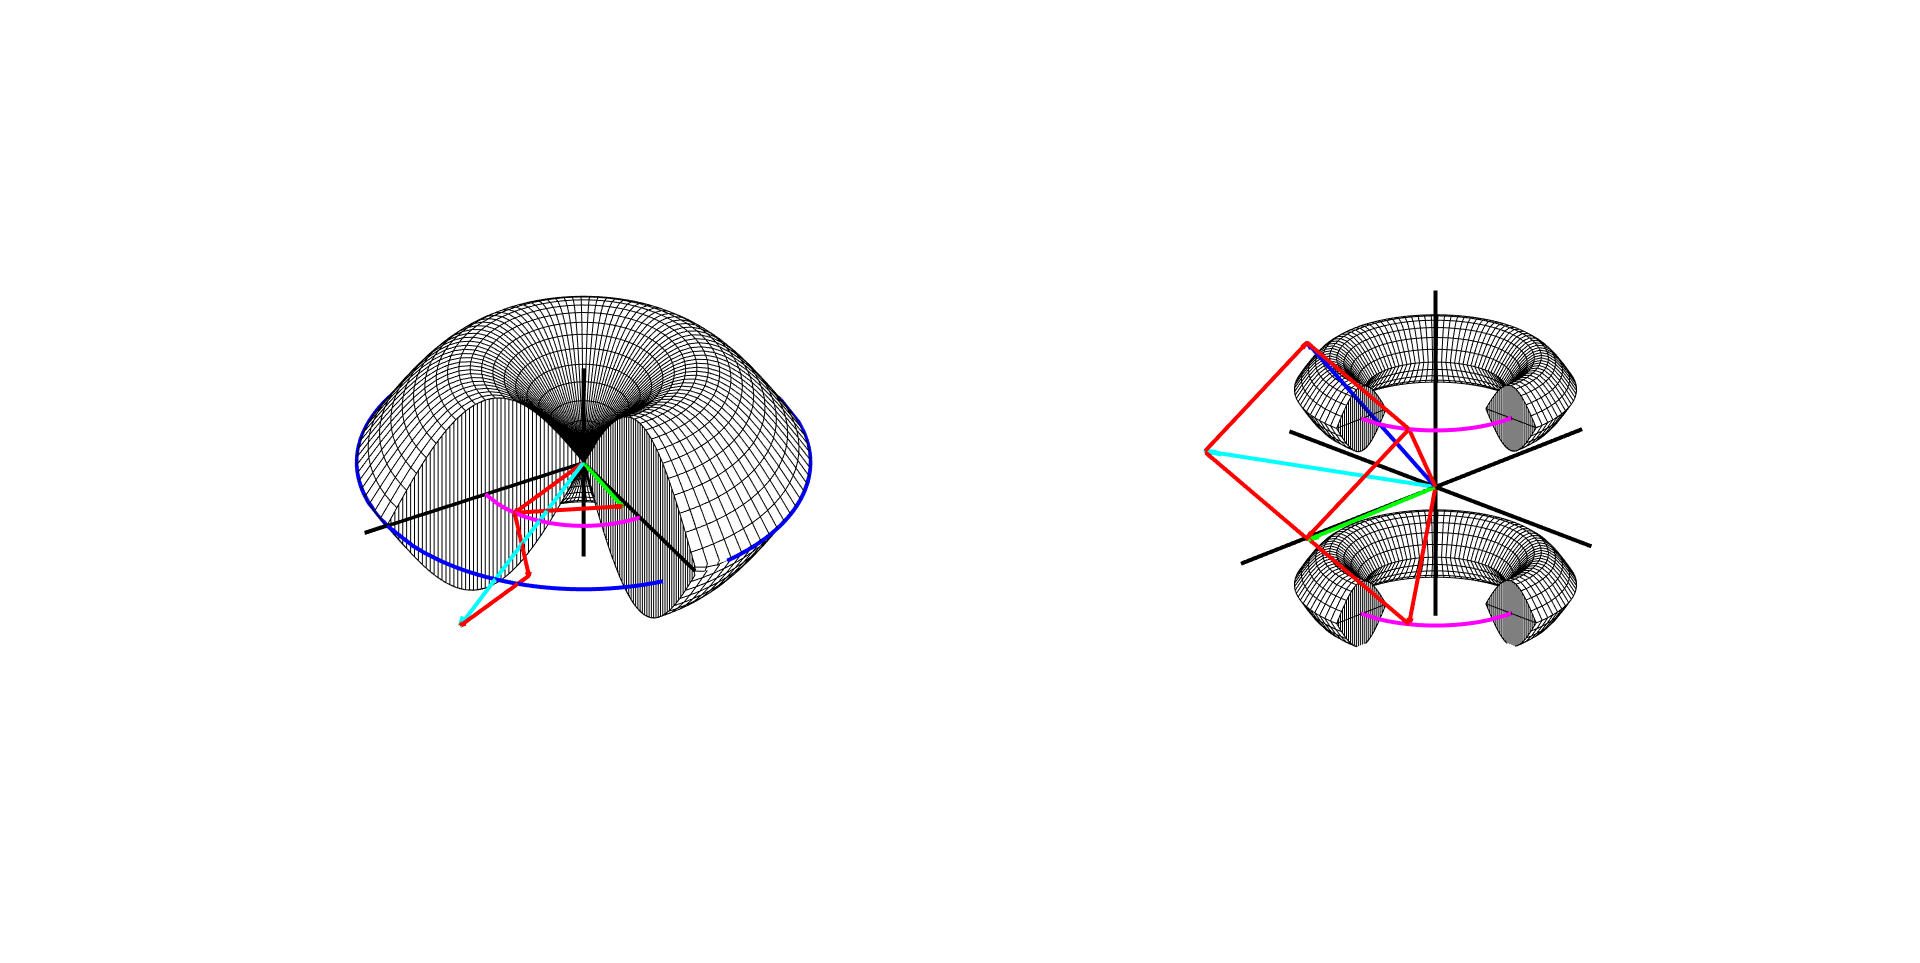
\includegraphics[width=1\linewidth]{introduction/mode_coupling.png}
\captionstyle{normal}
\caption{Трехмерная иллюстрация области апериодической неустойчивости в пространстве волновых векторов (a) в отсутствие внешнего магнитного поля и (b) в достаточно сильном внешнем магнитном поле. Синяя линия соотвествует границе неустойчивости поперечных мод $|K_\perp|=\sqrt{A}$ в отсутствие внешнего магнитного поля, а розовая линия~-- оптимальным модам $\overrightarrow{K}_{opt}$. Красные линии демонстрируют примеры оптимальных волновых векторов, взаимодействие которых в значительной степени определяет генерацию мод (зеленый, бирюзовый и синий цвет) вне области линейной неустойчивости.
}
\label{ris:mode_coupling}
\end{figure}

В присутствии внешнего магнитного поля $b_{ext}$ имеются две неустойчивые ветви: так называемые "периодическая"~ и "апериодическая"\cite{???}. Моды, направленные преимущественно вдоль внешнего магнитного поля, а значит, и оси анизотропии, относят к периодическим, поскольку их линейный инкремент мал в сравнении с действительной частотой и в сравнении с линейным инкрементом мод другой ветви~\cite{Li2000}. Поэтому влияние "периодической"~ ветви фактически не проявляется в расчетах методом частиц в ячейках, проводимых в настоящей работе, и не учитывается в приближенном квазилинейном описании.

Другую ветвь неустойчивости в литературе принято называть апериодической~\cite{???}, хотя нами показано, что в определенных условиях у ее линейно поляризованных мод присутствует действительная частота, увеличивающаяся с ростом внешнего магнитного поля $B_{ext}$ и уменьшением угла $\theta$ между волновым вектором $\vec{K}$ и этим магнитным полем. Область неустойчивости поперечных мод с увеличением внешнего поля достаточно быстро сужается,  как с длинноволновой, так и с коротковолновой стороны спектра, а линейный инкремент всех мод, остающихся неустойчивыми, уменьшается. В работе~\cite{Emelyanov2023_Radiophys} в пределе $\gamma\ll K_\perp\beta_\perp$, реализующемся при невысокой начальной анизотропии ($A_0\lesssim1$), либо при высокой анизотропии и внешнем магнитном поле, близком к подавляющему, область неустойчивости поперечных мод оценивалась как:
\begin{equation}
    K_\perp\in\left(\frac2{\sqrt{3}}\sqrt{A_0}\cos\left[\frac{\pi}3+\frac13\arccos\left(\frac{b_{ext}}{b_{s\perp}(A_0)}\right)\right];\frac2{\sqrt{3}}\sqrt{A_0}\cos\left[\frac{\pi}3-\frac13\arccos\left(\frac{b_{ext}}{b_{s\perp}(A_0)}\right)\right]\right),
    \label{eq:border_perp_inst}
\end{equation}
где $b_{s\perp}(A_0)$~--- нормированное магнитное поле, подавляющее неустойчивость поперечных мод, квадрат которого оценен в~\cite{Emelyanov2023_Radiophys} как:
\begin{equation}
    b_{s\perp}^2(A_0)=\frac{8\pi}{27}\frac{A_0^3}{1+A_0^3}<1.
    \label{eq:Emel_condition}
\end{equation}
По мере увеличения внешнего магнитного поля $b_{ext}$ монотонно уменьшается не только линейный инкремент всех поперечных мод, но и угол между внешним магнитным полем и волновым вектором моды с наибольшим инкрементом~(рис. \ref{ris:mode_coupling}b)~\cite{Moya2022,Li2000,Camporeale2008}. Таким образом, для наклонных мод неустойчивость может развиваться при $b_{ext}>b_{s\perp}(A_0)$. Вводя величину магнитного поля $b_s(A_0)$, при которой апериодическая неустойчивость полностью подавлена, приведем оценку для неё из работы~\cite{Hellinger2014}, аппроксимирующую численно полученный порог неустойчивости в диапазоне значений начальной анизотропии $A_0$ от $0.2$ до $9$:

\begin{equation}
    b_{s}^2(A_0)=\left(\frac{A_0}{1.27(1+A_0)}\right)^{\frac1{0.954}}.
    \label{eq:Hellinger_condition}
\end{equation}
\begin{figure}[h]

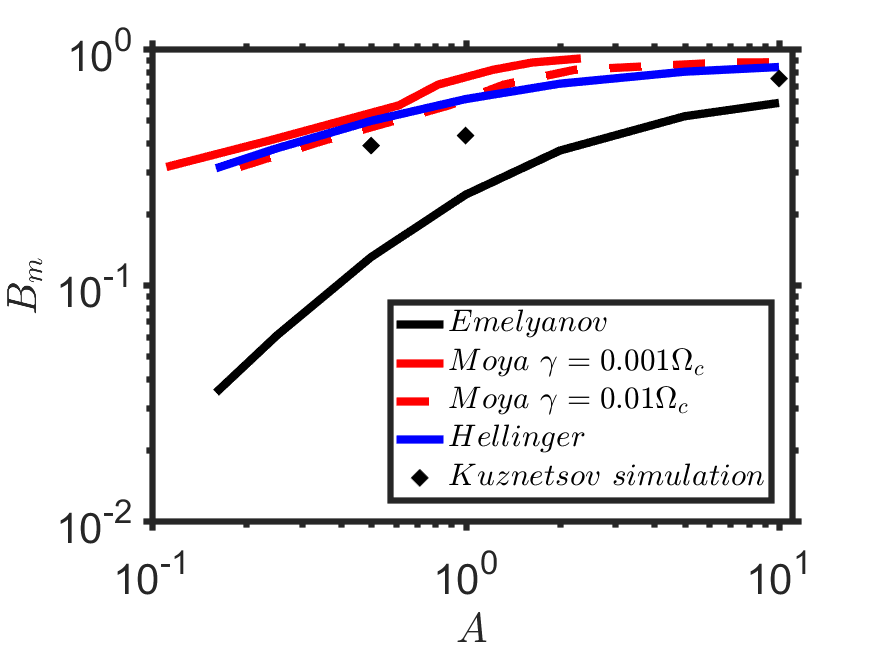
\includegraphics[width=0.5\linewidth]{introduction/b_podavl12.png}
\centering
\captionstyle{normal}
\caption{Зависимость подавляющего внешнего магнитного поля от начальной анизотропии для поперечных апериодических мод~(\ref{eq:Emel_condition}) (черный цвет), всех апериодических мод согласно оценке~(\ref{eq:Hellinger_condition}) (синий цвет) и согласно результатам расчетов~\cite{Moya2022} (красный цвет).}

\label{ris:B_podavl}
\end{figure}

Сравнение оценок (\ref{eq:Emel_condition}) и (\ref{eq:Hellinger_condition}) показывает, что если при высоких начальных анизотропиях отношение $ b_{s}^2/ b_{s\perp}^2$ лишь немного превышает единицу, то при низких начальных анизотропиях оно может составлять несколько порядков~(рис. \ref{ris:B_podavl}). Значит, существует широкий диапазон параметров, в котором принципиально важен учет наклонных мод, так как поперечные моды устойчивы в линейном приближении.

Первая глава работы содержит обсуждение уравнений и посвящена анализу вейбелевской турбулентности в одномерном случае, когда волновой вектор множества учитываемых коллинеарных неустойчивых мод направлен поперек оси анизотропии, т.\,е. вдоль оси $x$. Именно в этом направлении возбуждаются гармоники с наибольшими инкрементами. Для рассматриваемых ТМ-возмущений электрическое поле направлено вдоль оси анизотропии $y$, а магнитное -- вдоль оси $z$.  В данном разделе внимание сосредоточено на механизме возбуждения и насыщения гармоник ФР и магнитного поля, кратных исходной возбуждемой. Продемонстрирована квазилинейность задачи, обеспечивающая возможность пренебрежения высшими кратными гармониками магнитного поля при описании развития вейбелевской турбулентности. Проведено тщательное сравнение полученных численных результатов построенной квазилинейной одномерной модели вейбелевской турбулентности с более ранними аналитическими результатами работы~\cite{Pokhotelov2011}

Во второй главе используются аналогичные квазилинейные уравнения для двумерной задачи и приводятся результаты их решения в простейшем случае аксиальной симметрии, в котором температура частиц и все характеристики вейбелевской турбулентности изотропны в плоскости $xz$, т.е. спектр зависит только от радиальной компоненты $k$ волнового вектора. Эти результаты, полученные для случая двумерной аксиально симметричной турбулентности, сравниваются с полученными методом частиц в ячейках при помощи кода EPOCH~\cite{Arber2015}, учитывающего и более тонкие нелинейные эффекты, в том числе четырехволновое взаимодействие. 

В третье главе при помощи того же квазилинейного приближения описано совместное развитие двухпотоковой (ленгмюровской) и вейбелевской кинетических неустойчивостей в плазме с пучком частиц. Будет показано, что развивающаяся вейбелевская турбулентность магнитного поля может значительно деформировать резонансную с ленгмюровскими волнами область распределения частиц по скоростям, существенно влияя тем самым на формирование и особенно затухание ленгмюровской турбулентности. Ленгмюровская турбулентность электрического поля, в свою очередь, способна существенно изотропизовать распределение частиц по скоростям, а следовательно, изменить инкременты, характер эволюции и уровень насыщения гармоник вейбелевской турбулентности.

В четвертой главе проанализировано  изменение эволюции распределения частиц по скоростям, среднеквадратичного магнитного поля, его спектра в целом и отдельных гармоник в частности с увеличением величины внешнего магнитного поля от малого до почти подавляющего неустойчивость для представительного диапазона величин начальной анизотропии распределения частиц по скоростям. Основное внимание уделяется описанию  процессов нелинейного, в частности, трех- и четырехволнового взаимодействия между модами. В заключительном разделе суммируются общие свойства эволюции квазимагнитостатической турбулентности, генерируемой шланговой неустойчивостью во внешнем магнитном поле, и обсуждается возможная роль этой турбулентности в формировании корональных вспышек на Солнце и звездах поздних спектральных классов.

В пятой главе рассматривается аналогичная постановка задачи для\\ бикаппа-распределения~\cite{Livadiotis2017, Livadiotis2021}, выбранного в качестве начального. Оно свойственно неравновесной плазме, частицы которой испытали стохастическое ускорение под действием того или иного широкополосного электромагнитного излучения, например в звездном ветре или различных ударных волнах, и в качестве частного случая содержит бимаксвелловское распределение частиц по скоростям. Исследования нелинейной стадии вейбелевской неустойчивости для начального бикаппа-распределения ранее отсутствовали.



    % Введение
\ifnumequal{\value{contnumfig}}{1}{\counterwithout{figure}{chapter}
}{\counterwithin{figure}{chapter}}
\ifnumequal{\value{contnumtab}}{1}{\counterwithout{table}{chapter}
}{\counterwithin{table}{chapter}}
\chapter{Эволюция одномерной вейбелевской турбулентности}\label{ch:ch1}
\section{Адиабатическая динамика мод и схема их связи в условиях слабого четырехволнового взаимодействия}\label{sec:ch1/sec1}

Для бесстолкновительной плазмы, в которой на рассматриваемых временах эволюции вейбелевской турбулентности можно пренебречь движением тяжелых ионов, самосогласованные уравнения  Максвелла~-- Власова для электрического $\vec{E}=(0, E_y, 0)$ и магнитного $\vec{B}=(B_x, 0, B_z)$ полей и функции распределения электронов $f(v_x , v_y , v_z, x, z, t)$ имеют вид
\begin{align}
    \nabla \times \vec{B}=\dfrac{1}{c}\dfrac{\partial \vec{E}}{\partial t}+\dfrac{4\pi}{c}\vec{j}, \\
    \nabla \times \vec{E}=-\dfrac{1}{c}\dfrac{\partial \vec{B}}{\partial t}, \\
    \dfrac{\partial f}{\partial t}+\vec{v}\dfrac{\partial f}{\partial \vec{r}}+\dfrac{e}{\me} \left(\vec{E}+\dfrac{1}{c}\left[\vec{v},\vec{B}\right]\right) \dfrac{\partial f}{\partial \vec{v}}=0,
\end{align}
где $c$~--- скорость света в вакууме, $e$ и $\me$~--- заряд и масса электрона, $\vec{j}=e\iiint^{+\infty}_{-\infty}\vec{v}f(v_x , v_y , v_z, x, z, t) dv_x dv_ydv_z$~--- плотность тока, $N=\iiint^{+\infty}_{-\infty}f(v_x , v_y , v_z , x, z, t)dv_xdv_ydv_z$~--- концентрация электронов. Здесь и ниже речь идет о так называемых ТЕМ-возмущениях, в которых взаимно ортогональны друг к другу волновой вектор и магнитное и электрическое поля, причем последнее параллельно оси анизотропии плазмы. При этом выше учтено, что для двумерной задачи радиус-вектор является двухкомпонентным, $\vec{r}=(x , 0 , z)$, а вектор скорости~--- трехкомпонентным,  $\vec{v}=(v_x , v_y ,v_z)$ (в одномерной задаче отсутствуют зависимости от координаты $z$ и скорости $v_z$, но сохраняются зависимости от двух других компонент $v_x$, $v_y$). 

Положим, что в начальный момент времени нормированная функция распределения по скоростям $c^3f/N$ имеет бимаксвелловский вид:
\begin{equation}
\label{bimax}
\Psi(\beta)=\dfrac{1}{\pi^{3/2}\beta_{\perp0}^2 \beta_{\|0} } \exp\left(-\dfrac{\beta_x^2+\beta_z^2}{\beta_{\perp0}^2}-\dfrac{\beta_y^2}{\beta_{\|0}^2}\right).
\end{equation}
Здесь $\beta_{x,y,z}={v_{x,y,z}}/{c}$, т.\,е. $\beta=\vec{v}/{c}$, и в дальнейшем используется параметр анизотропии $A_0={\beta^2_{\|0}}/{\beta^2_{\perp0}}-1$, определяемый отношением большей тепловой скорости к меньшей.

Квазилинейный подход к описанию ТЕМ-вейбелевской неустойчивости основан на разложении по пространственным модам (гармоникам) решения уравнений  Максвелла~-- Власова~\cite{Baumjohann2012} с шумоподобным начальным возмущением магнитного поля, обладающим примерно равномерным спектром в области неустойчивых волновых чисел мод. Особенно эффективным подобное разложение является тогда, когда ключевую роль играет интегральное нелинейное взаимодействие мод посредством их совместного изменения средней по пространству функции распределения частиц по скоростям. Для вейбелевской турбулентности это оправдано ввиду слабой нелинейности кинетического уравнения Власова в рассматриваемых условиях отсутствия квазимонохроматических электромагнитных волн и их резонансного взаимодействия~\cite{Kuznetsov2022}. В частности, как показали тестовые расчеты, для любой отдельной гармоники магнитного (и соответствующего электрического) поля $B_1(t,x)= \mathrm{Re} \left[ B_1(t)\exp(-\mathrm{i}kx) \right]$ с волновым вектором $\vec{k}$, для определенности направленным вдоль орта $\vec{x_0}$, можно не учитывать кратные гармоники $\ell k$ с целым $\ell > 1$ и необходимо учесть только три гармоники поправок к функции распределения, $\delta f_\ell(t, x)=\mathrm{Re} \left[ f_\ell(t)\exp(-\mathrm{i}\ell kx) \right]$, со значениями $\ell =$ 0, 1, 2. При этом возбуждение чётной гармоники $\ell=$ 2 магнитного поля фактически невозможно благодаря ограничениям симметрии в одномерной и аксиально симметричной двумерной задачах. Здесь и ниже $\vec{x}_0$, $\vec{y}_0$, $\vec{z}_0$~--- единичные орты декартовой системы координат. 

Наличие большого числа однотипных не сфазированных мод, достаточно плотно заполняющих значимую область волновых векторов, гарантирует гладкость формы и плавность изменения функции распределения, исключая артефакты когерентной интерференции и отрицательные значения функции распределения электронов всюду, кроме, возможно, несущественной, содержащей крайне мало частиц, области их скоростей, очень больших по сравнению с тепловыми скоростями. При этом по существу реализуется адиабатическая динамика каждой моды, непрерывно подстраивающейся к изменяющейся функции распределения частиц. Корректность такого рода теории возмущений, а фактически~--- соблюдение иерархии малости амплитуд последующих гармоник по сравнению с предыдущими (как гармоник функции распределения, $|\delta f_ \ell|\gg |\delta f_{\ell+1}|$, так и аналогичных гармоник магнитного или электрического полей) проверены нами в случаях задания одной или двух производящих мод. 

Так, в случае единственной производящей моды нелинейно связываются все кратные гармоники функции распределения $\ell k$ с $\ell =$ 0, 1, 2, 3,~... и нечетные гармоники ТЕМ-поля $\ell k$ с $\ell =$ 1, 3,~... (в силу отсутствия токов на четных гармониках из-за свойств четности функции распределения), но учет высших гармоник, начиная с $\ell =$ 3, почти не изменяет результат.  Удостовериться в этом позволяет следующая система связанных уравнений для кратных (комплексных) гармоник-возмущений функции распределения, отвечающая теории возмущений до $\ell = 4$:
% \begin{wide}
\begin{align}
    \label{eq:furre5}
    \vec{B} = \mathrm{Re} \left[ B_1(t) \exp(-\mathrm{i}kx)+B_3(t)\exp(-3\mathrm{i}kx)\right] \vec{z_0} ,\\
% \end{align}
% \begin{align}
\label{eq:f0.1}\dfrac{\partial f_0}{\partial t}+\hat \phi(\Omega_1,f_1^*)+\hat \phi^*(\Omega_1^*,f_1)+\hat \phi(\Omega_3,f_3^*)+\hat \phi^*(\Omega_3^*,f_3)=0,\\
% \end{align}
% \begin{align}
\label{eq:f1.1}\dfrac{\partial f_1}{\partial t}+\mathrm{i}kv_xf_1+2\hat \phi(\Omega_1,f_0)+\hat \phi^*(\Omega_1^*,f_2)+\hat \phi(\Omega_3,f_2^*)=0,\\
% \end{align}
% \begin{align}
\label{eq:f2.1}\dfrac{\partial f_2}{\partial t}+2\mathrm{i}kv_xf_2+\hat \phi(\Omega_1,f_1)+\hat \phi^*(\Omega_1^*,f_3)+\hat \phi(\Omega_3,f_1^*)=0,\\
% \end{align}
% \begin{align}
\label{eq:f3.1}\dfrac{\partial f_3}{\partial t}+3\mathrm{i}kv_xf_3+2\hat \phi(\Omega_3,f_0)+\hat \phi^*(\Omega_1^*,f_4)+\hat \phi(\Omega_1,f_2)=0,\\
% \end{align}
% \begin{align}
\label{eq:f4.1}
\dfrac{\partial f_4}{\partial t}+4\mathrm{i}kv_xf_4+\hat \phi(\Omega_1,f_3)+\hat \phi(\Omega_3,f_1)=0,
\end{align}
% \end{wide}
где опущены очевидные осцилляторные уравнения для первой и третьей гармоник магнитного поля (\ref{eq:furre5}), получающиеся из уравнений (\ref{eq:maxw1}), (\ref{eq:maxw2}) и в силу их линейности включающие только соответствующие первую и третью гармоники функции распределения. Для сокращения записи здесь введён оператор
\begin{align}
\label{eq:oper.1}
    \hat{\phi}(\Omega_{n},f(\vec{v}))  =  \frac{\mathrm{i}}{2nk}\cdot\frac{\partial \Omega_{n}}{\partial t}\frac{\partial f(\vec{v})}{\partial v_y} -\frac{1}{2}\Omega_{n} \left(v_x\frac{\partial f(\vec{v})}{\partial v_y}-v_y\frac{\partial f(\vec{v})}{\partial v_x}\right)
\end{align}
и комплексная гирочастота $\Omega_n={e B_n}/{(\me c)}$. Данная система схематически представлена на рис.~\ref{fig:1m2pribl_1}, а результат прямой проверки корректности ее решения путем сравнения с решением исходных уравнений (\ref{eq:maxw1})--(\ref{eq:Vlasov}) кодом EPOCH при начальном возбуждении одной сильной моды существенно выше уровня шумов продемонстрирован на рис.~\ref{fig:srav_PIC} (решения совпадают с точностью до нескольких процентов). В качестве неявной проверки слабой генерации высших гармоник в полученной системе уравнений было показано, что ее численное решение для основной гармоники (моды) магнитного поля $B_1(t)$, непосредственно создаваемой первой гармоникой функции распределения $f_1(t)$, практически не отличается от численного решения значительно упрощенной системы, в которой эволюция данной гармоники $B_1(t)$ (и $f_1(t)$) определяется лишь согласованной динамикой нулевой и второй гармоник функции распределения $f_0,_2(t)$, но не третьей (и высшими) гармониками магнитного поля и функции распределения.

\begin{figure}[t]
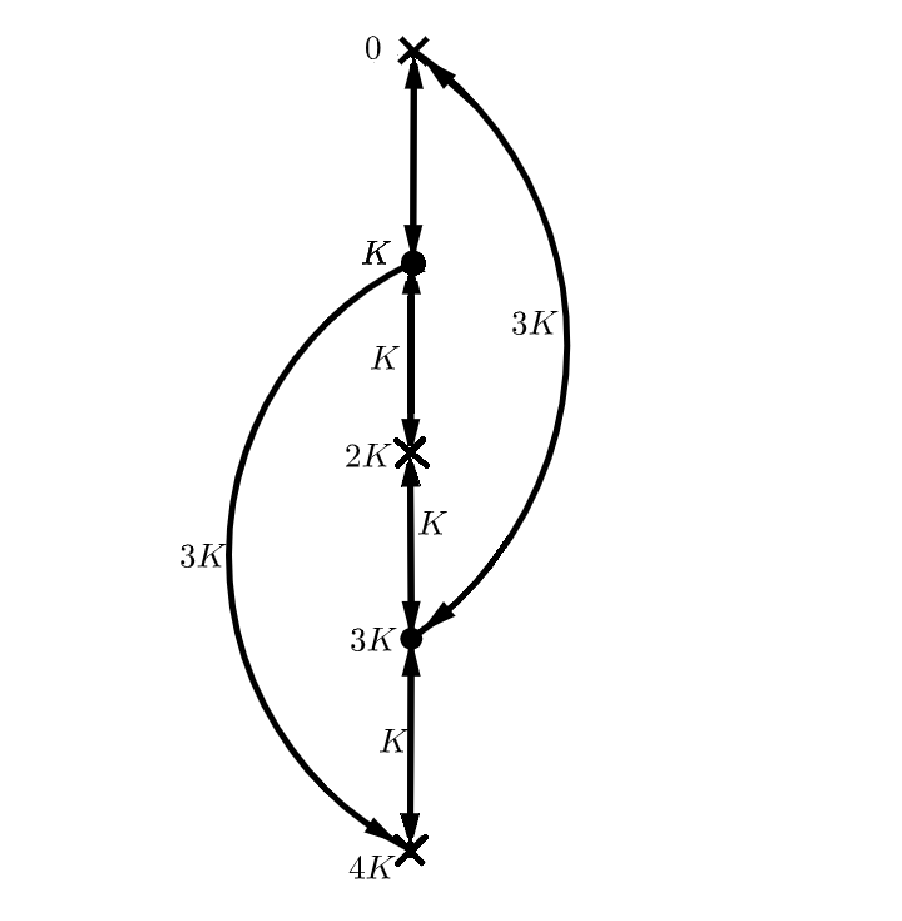
\includegraphics[width=0.4\linewidth]{part1/fig1.eps}
\centering
\caption{Схема связи четырех гармоник функции распределения частиц в самосогласованной системе уравнений (\ref{eq:furre5})--(\ref{eq:f4.1}) для одной производящей моды. Узел на схеме отвечает уравнению на соответствующую гармонику. Если поле некоторой гармоники тождественно равно нулю, то соответствующий узел изображен в виде крестика, а если нет~--- в виде точки. Входящая в узел стрелка отвечает слагаемому в уравнении для гармоники, соответствующей этому узлу. В таком слагаемом присутствует гармоника поля, соответствующая гармонике, указанной на стрелке, и гармоника функции распределения частиц, указанная на узле, из которого стрелка исходит.} 
\label{fig:1m2pribl_1}
\end{figure}

В общем случае многомодовой динамики вейбелевской неустойчивости неизбежно возникают перекрестные гармоники вида $k_i\pm k_j$, $2k_i\pm k_j$ и т.д. Схема взаимосвязи подобных перекрестных гармоник в случае наличия двух производящих вейбелевских мод дана на рис.~\ref{fig:2m2pribl}. Подобно одномодовой иллюстрации корректности пренебрежения кратными гармониками, нами была показана слабость генерации перекрестных гармоник на основе сравнения решений полной системы уравнений и значительно сокращенной системы, содержащей гармоники не выше второго порядка, включая суммарные и разностные, в случае начального задания только двух сильных мод. Учет четырехволнового взаимодействия мод в подобной системе квазилинейных уравнений является крайне громоздким и выходит за рамки статьи.


\begin{figure}[b]
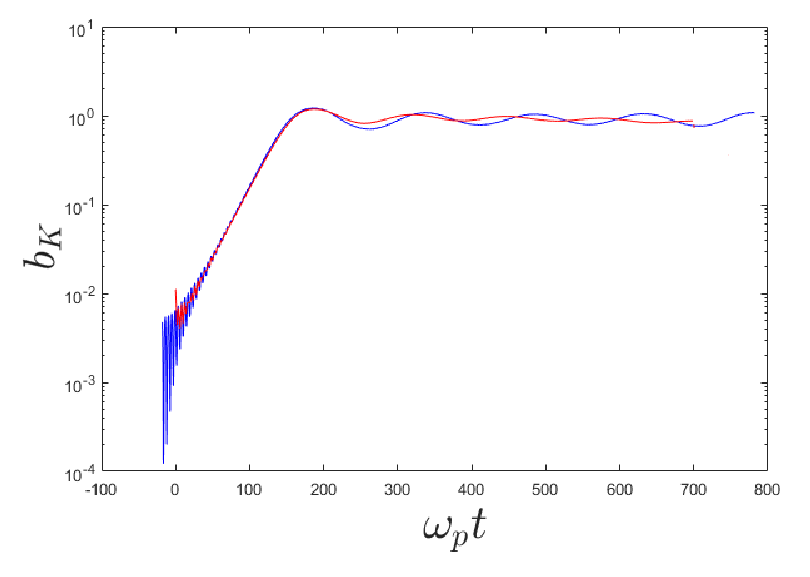
\includegraphics[width=0.5\linewidth]{part1/fig2.eps}
\centering
\caption{Эволюция одной моды: сравнение хода амплитуды основной гармоники магнитного поля в квазилинейном расчете по уравнениям (\ref{eq:f0.1})--(\ref{eq:f4.1}) (синий цвет) и в расчете методом частиц в ячейках с помощью кода EPOCH по уравнениям (\ref{eq:maxw1})--(\ref{eq:Vlasov}) (красный цвет) при $A_0=10$, $K=1.2$.}
\label{fig:srav_PIC}
\end{figure}

Итак, имеем следующую квазилинейную систему уравнений для одномерной вейбелевской турбулентности с большим числом $m$ коллинеарных мод $\{ k_1,\, k_2,...,\,k_{m} \}$, волновые векторы которых направлены поперек оси анизотропии, часто расположены и перекрывают всю существенную область неустойчивости: 
% \begin{wide}
\begin{align}
 %(\ref{eq14})--(\ref{eq19}) из $5m\cdot s+1$ обезразмеренных уравнений
\label{eq:f0.3}
\dfrac{\partial \psi_0}{\partial \tau}+\sum\limits^{m}_{n=1}\bigg(\hat \Phi(b_{K_n},\psi_{K_n}^*)+\hat \Phi^*(b_{K_n}^*,\psi_{K_n})\bigg)=0, \\
% \end{align}
% \begin{align}
\label{eq:f1.3}
\dfrac{\partial \psi_{K_n}}{\partial \tau}+\mathrm{i}K_n\beta_x\psi_{K_n}+2\hat \Phi(b_{K_n},\psi_0)+\hat \Phi^*(b_{K_n}^*,\psi_{2K_n})=0, \\
% \end{align}
% \begin{align}
\label{eq:f2.3}
\dfrac{\partial \psi_{2K_n}}{\partial \tau}+2\mathrm{i}K_n\beta_x\psi_{2K_n}+\hat \Phi(b_{K_n},\psi_{K_n})=0,\\
% \end{align}
% \begin{align}
\label{eq:max_eq}
\ddot b_{K_n}+K_n^2b_{K_n}=\dfrac{\mathrm{i}K_n}{\beta_{||0}}\iint\limits^{\infty}_{-\infty}\beta_y\psi_{K_n}(\tau,\beta_x,\beta_y) d\beta_x d\beta_y.
\end{align}
% \end{wide}
Согласно ей, магнитное поле имеет вид суммы мод по целочисленному индексу $n$:
$B(t,x)= \mathrm{Re} \, \sum^{m}_{n=1}B_{k_{\vec{n}}}(t)\exp(- ik_{n}x)$.
Аналогичный вид имеет каждая из двух кратных гармоник-возмущений функции распределения частиц по скоростям, т.\,е. компонент $\delta f_1(t,x)$ и $\delta f_2(t,x)$, разложенных на комплексные гармоники ${f_1}_{k_{\vec{n}}}(t)$ и ${f_2}_{k_{\vec{n}}}(t)$ соответственно; нулевая (действительная) гармоника $f_0(t)=\delta f_0(t)$ зависит только от вектора скорости и дает поправку к функции распределения, усредненную по оси $x$. Здесь и ниже используются время и волновое число, нормированные на плазменные частоту и масштаб,
\begin{align}
\label{eq19plus2}
    \tau=\wpl t, \
    K=\dfrac{kc}{\wpl}; \ 
    \wpl^2=\dfrac{4\pi Ne^2}{\me}.
\end{align}
% \begin{multicols}{2}
Комплексные амплитуды мод (гармоник) магнитного поля и функции распределения тоже нормированы:
\begin{figure}[b]
\centering
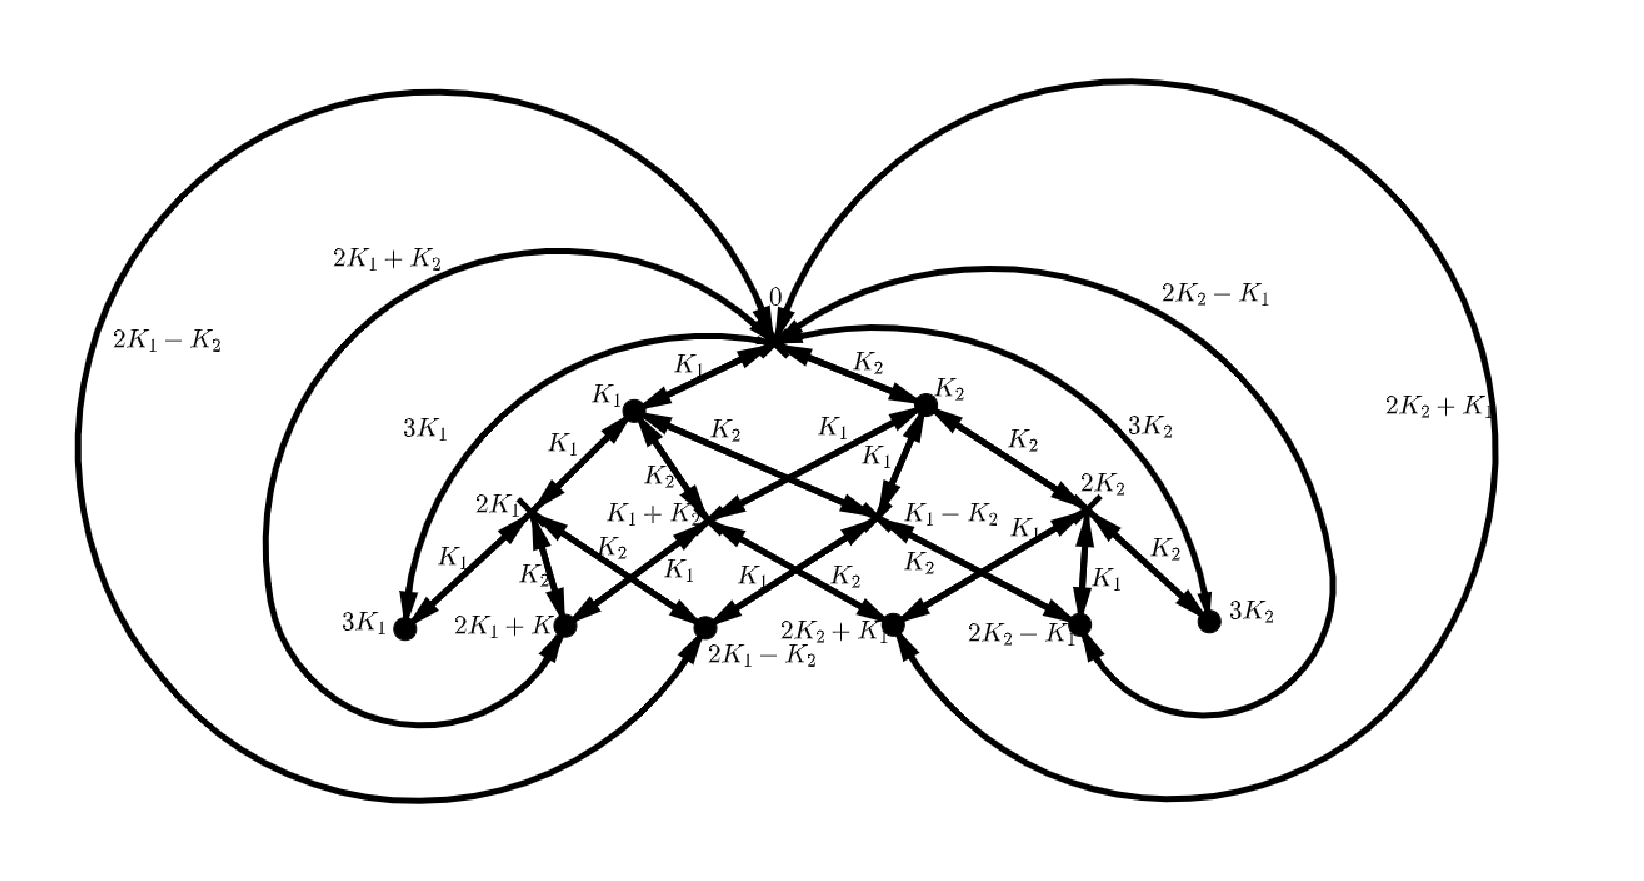
\includegraphics[width=1\linewidth]{part1/fig3.eps}
\caption{Схема связи гармоник функции распределения в самосогласованной системе уравнений для двух производящих мод. Обозначения те же, что на рис.~\ref{fig:1m2pribl_1}.}
\label{fig:2m2pribl}
\end{figure}


\begin{align}
\label{eq19plus1}
    b_{K_{n}}=\dfrac{B_{K_{n}}}{\sqrt{8\pi N T_{\|0}}},\
    T_{\|0}=\dfrac{m_ec^2\beta_{\|0}^2}{2},\  \psi_{\ell\cdot K_{n}}=\dfrac{c^2f_{\ell\cdot K_{n}}}{N},
    \ \ell=0,\,1,\,2.  
\end{align}
Для многомодовой задачи введен оператор 
\begin{align}
\label{eq:oper.2}\hat \Phi(b_{K_n},\psi(\beta)) =  \dfrac{\mathrm{i}}{2K_n}\dfrac{\partial b_{K_n}}{\partial \tau}\dfrac{\partial \psi(\beta)}{\partial \beta_y} -\dfrac{1}{2}b_{K_n} \left(\beta_x\dfrac{\partial \psi(\beta)}{\partial \beta_y}-\beta_y\dfrac{\partial \psi(\beta)}{\partial \beta_x}\right) ,
\end{align}
отличающийся нормировкой переменных и параметров от указанного ранее оператора (\ref{eq:oper.1}) в одномодовой задаче. Квадратичные слагаемые в уравнениях обуславливают квазилинейное взаимодействие между не скоррелированными по фазам модами. Оно осуществляется посредством их коллективного, нелинейного воздействия на однородную компоненту функции распределения, приводящего к изменению ее формы, снижению анизотропии распределения, появлению ненулевых действительных частот мод и их декрементов, т.е. смене знака их инкрементов, и, как следствие, насыщению неустойчивости. Для применимости теории слабой турбулентности~\cite{Krall1975,Vedenov1962} в рассматриваемой задаче необходима как справедливость сформулированной теории возмущений, так и возможность на нелинейной стадии эволюции использовать для мод линейное дисперсионное уравнение, которое содержит текущую функцию распределения частиц по скоростям, усреднённую по пространству и отличную от начальной.


\section{Эволюция одномерной вейбелевской турбулентности}\label{sec:ch1/sec2}

Одномерная эволюция большого числа сонаправленных вейбелевских мод, плотно покрывающих область неустойчивости, определяется представленной системой уравнений (\ref{eq:f0.3})--(\ref{eq:max_eq}) с оператором (\ref{eq:oper.2}) при задании величины начальной анизотропии бимаксвелловской плазмы $A_0$, одной из тепловых скоростей, например $\beta_{\perp0}$, и начального спектра мод функции распределения и электромагнитного поля. Ключевым параметром нелинейного развитие динамического спектра турбулентности является начальная анизотропия $A_0$, задающая, в частности, линейный спектр неустойчивых вейбелевских мод, т.е. их инкременты. При $A_0\ll1$ максимальный инкремент (в единицах $\omega_p$) равен $\gamma_\mathrm{max}\approx 2 \beta_{\perp0} (A_0 / 3)^{3/2}$ и достигается для оптимального волнового числа $К_\mathrm{opt} \approx (A_0 / 3)^{1/2}$, при $A_0 \gg 1$ имеем $\gamma_\mathrm{max} \approx \beta_{\perp0} \left( \left[ (A_0+1)/2 \right]^{1/2} - 1 \right)$ для $K_\mathrm{opt} \approx \left( \left[ (A_0+1)/2 \right]^{1/2} - 1 \right)^{1/2}$. Ниже отдельно обсуждаются случаи низкой ($A_0 = 0.25$) и высокой ($A_0 = 10$) начальной анизотропии. В~обоих случаях получаются вполне сравнимые интегральные характеристики турбулентности, вычисляемые с использованием квазилинейных расчетов и моделирования методом частиц в ячейках при помощи кода EPOCH. Однако количественно результаты последнего, как правило, отличаются в полтора-два раза, поскольку в одномерной задаче он вносит сильные шумы в несвойственные ей компоненты полей и скоростей, заметно искажающие функцию распределения частиц, а следовательно, квазилинейную эволюцию спектра (другие нелинейные эффекты, в том числе, четырехволновые, для одномерной турбулентности не характерны).
 

Согласно~\cite{Nechaev2023}, на основе энергетических инвариантов~\cite{Davidson1972} для рассматриваемой одномерной задачи может быть получено следующее приближенное аналитическое соотношение между текущими значениями нормированного среднеквадратичного магнитного поля $b_{av}$, характерного волнового числа $\langle K\rangle$ \footnote{Во многих случаях представленному соотношению немного лучше удовлетворяет волновое число $K_\mathrm{max}(t)$, отвечающее максимуму спектра турбулентности, а не указанное выше число $\langle K\rangle$, усредненное
по спектру мод $b_{k}$, хотя эти числа довольно близки.} и параметра анизотропии плазмы $A$ (отличного от введенного в~\cite{Nechaev2023}), если считать, что пространственный спектр вейбелевской турбулентности достаточно узок:
\begin{equation}
\label{eq:otsenka}
b_{av}^2 = \frac{A_0-A}{1+A_0} \cdot \dfrac{0.5\langle K\rangle^2}{A \langle K\rangle^2 + A + 3 \langle K\rangle^2 + 2},
\end{equation}
\begin{equation}
\label{eq:angles}
\langle...\rangle=\frac{\int...b_k dk}{\int b_k dk} ,
\end{equation}
\begin{equation}
\label{eq:A_1d}
A=\frac{\iint\limits^{\infty}_{-\infty}\beta_y^2\psi_{0}(\tau,\beta_x,\beta_y) d\beta_x d\beta_y}{\iint\limits^{\infty}_{-\infty}\beta_x^2\psi_{0}(\tau,\beta_x,\beta_y) d\beta_x d\beta_y}-1 .
\end{equation}

Для представленных результатов моделирования одномерной турбулентности, согласованной со сложно меняющейся (не бимаксвелловской) функцией распределения частиц, это соотношение оказалось хорошо выполняющимся, обычно с точностью до нескольких процентов.
\subsection{Низкая начальная анизотропия}\label{subsec:low_A_1d}

Результаты имеющейся аналитической квазилинейной теории~\cite{Pokhotelov2011}, приближенно справедливой в одномерной задаче при малом параметре анизотропии $A\ll 1$, но не описывающей эволюцию турбулентности в явном виде и не учитывающей деформацию функции распределения частиц по скоростям вдоль оси анизотропии, трудно непосредственно сопоставить с приведенным выше соотношением и с прямым численным моделированием динамики спектра. Однако проведенное нами косвенное сопоставление показывает, что качественно эта теория вполне совместима с получаемыми более точными численными результатами в области ее применимости. Основные приближения аналитической квазилинейной теории~\cite{Pokhotelov2011} состоят в малости инкрементов, $\gamma_{K_n}\ll K_n\beta_{\perp0}$, и в узости области изменения усредненной в пространстве функции распределения частиц по скоростям, $\delta \beta_x\ll \beta_{\perp0}$. Первое требование призвано гарантировать применимость используемого дисперсионного уравнения, а второе фактически сводится к указанному условию $A\ll 1$. 

Интересующее нас косвенное сопоставление удается провести с использованием найденного в аналитической теории эволюционного параметра $h$, величина которого определяется адиабатической динамикой мод и однозначно задает вид деформированной функции распределения: 
 
\begin{equation}
\label{eq:b_eq}
|\dot b_{K_n}|=\gamma_{K_n}|b_{K_n}|, 
\end{equation}
\begin{equation}
\label{eq:h_def}
h=\sum_{K_n}\dfrac{|b_{K_n}|^2}{K_n^2}.
\end{equation}
\begin{figure}[b]
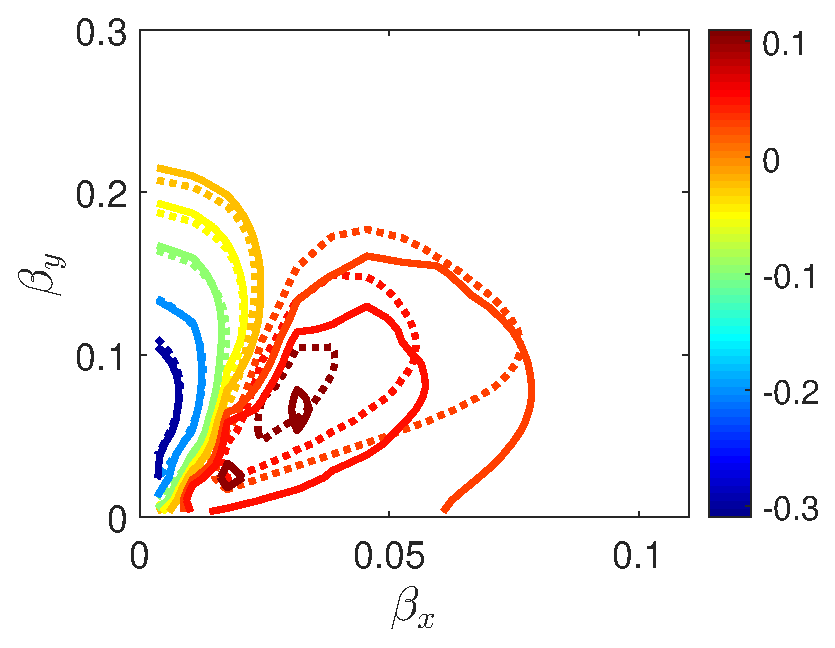
\includegraphics[width=0.5\linewidth]{part1/fig4.eps}
\centering
\caption{Построенные на основе 1-мерного квазилинейного расчета (сплошная линия) и вычисленные на основе аналитической теории~\cite{Pokhotelov2011} (пунктир) для момента времени $\wpl t = 9000$ линии уровня $-0.3$, $-0.2$, $-0.1$, $-0.05$, $-0.025$, $0.025$, $0.05$ и $0.1$ поправки к однородной компоненте функции распределения (\ref{bimax}), которая в начальный момент времени являлась бимаксвелловской с параметром анизотропии $A_0=0.25$. }
\label{fig:sravnenie_FR1d}
\end{figure}
На рис.~\ref{fig:sravnenie_FR1d} показана характерная деформация функции распределения частиц, происшедшая спустя время $\wpl t = 9000$ (т.е. примерно втрое позже начала заметного насыщения роста энергии турбулентного магнитного поля) и найденная как непосредственно из численного решения квазилинейной системы уравнений (\ref{eq:f0.3})--(\ref{eq:max_eq}), так и косвенно из аналитической квазилинейной теории (\ref{eq:b_eq})--(\ref{eq:h_def}) с использованием указанного численного решения для вычисления эволюционного параметра $h$ при малой начальной анизотропии $A_0=0.25$. Как видим, относительная деформация функции распределения составляет доли процента и действительно происходит в области скоростей, меньших тепловой скорости. В этой области угол движения электронов относительно оси анизотропии $y$ в среднем заметно увеличивается, хотя качественное изменение траекторий с появлением баунс-осцилляций фактически происходит только для малой доли электронов со скоростями, лежащими вдоль оси анизотропии в небольшом конусе углов с раскрывом, сужающимся с уменьшением параметра анизотропии $A_0$. В целом, в результате насыщения вейбелевской неустойчивости функция распределения по скоростям уплощается в своей центральной части, теряя там бимаксвелловскую форму и приобретая более сложный (в дальнейшем слабо меняющийся) анизотропный вид, причем полный параметр анизотропии уменьшается очень мало, на величину порядка 1-2\%, сначала осциллируя, а потом оставаясь почти постоянным. 



\begin{figure}[b]
\centering
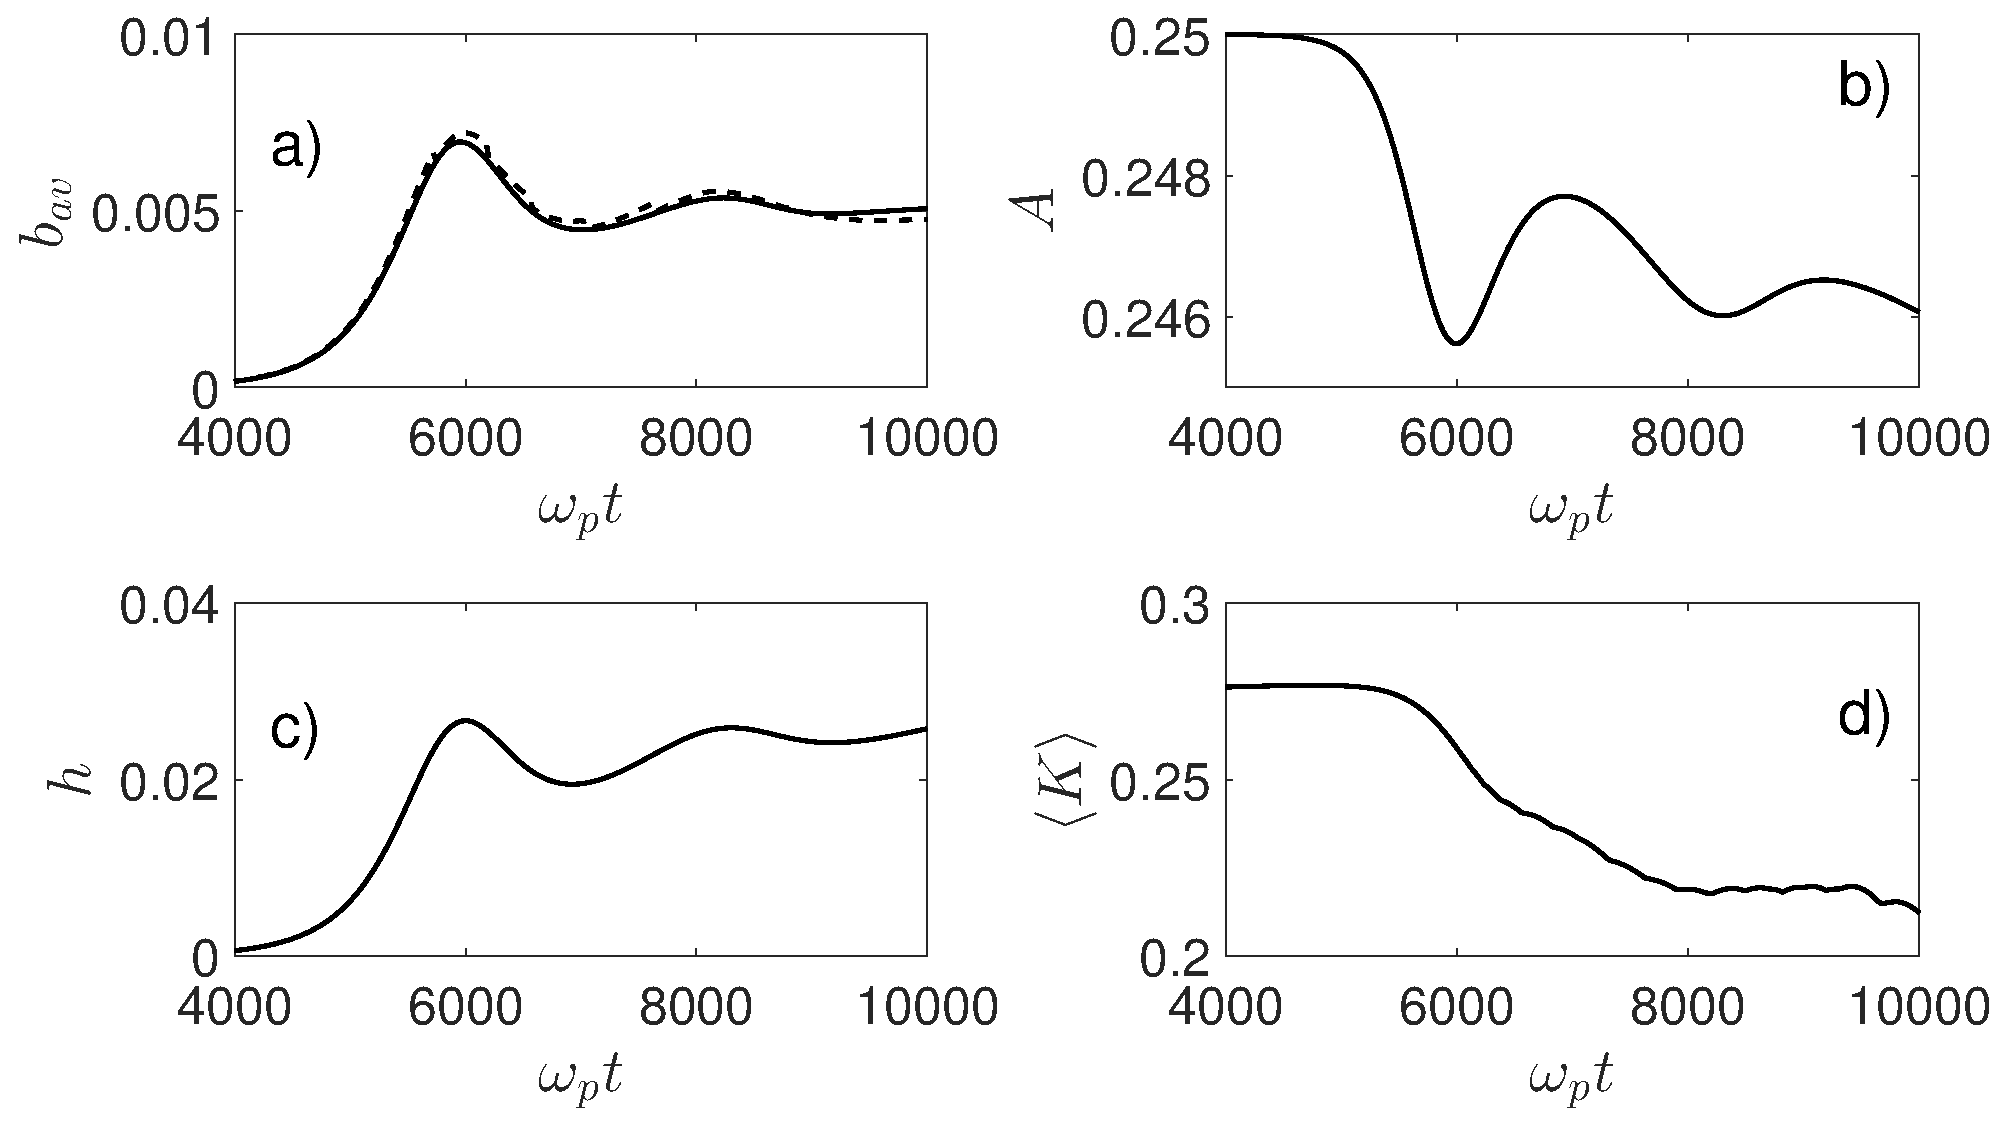
\includegraphics[width=0.9\linewidth]{part1/fig5.eps}
\caption{Эволюция (a) среднеквадратичного магнитного поля $b_{av}$ (сплошная линия) и оценки этой величины~(\ref{eq:otsenka})~(штрихи), (b) параметра анизотропии $A$, (c) эволюционного параметра $h$, (d) характерного, среднего волнового числа $\langle K\rangle$ согласно численному 1-мерному квазилинейному моделированию при $A_0=0.25$.}
\label{fig:evol1d_QL_A025}
\end{figure}
Несмотря на приближенный характер аналитической квазилинейной теории, ее отличия от более точного численного квазилинейного моделирования при сравнении величин среднеквадратичного магнитного поля $b_{av}$, эволюционного параметра $h$ и характерного волнового числа $\langle K\rangle$ на нелинейной стадии ($\wpl t > 3000$) не превышают $20\%$ (рис.~\ref{fig:evol1d_QL_A025}). Наибольшие расхождения наблюдаются в переходной области от быстрого экспоненциального роста к медленной квазилинейной эволюции. В отличие от ожидавшегося в аналитической теории плавно-монотонного изменения всех указанных величин, данный переход в численном квазилинейном моделировании, как и в расчетах методом частиц в ячейках, демонстрирует небольшие осцилляции этих величин (за исключением монотонного уменьшения характерного волнового числа примерно на четверть от исходного значения). Их средние значения после переходной стадии со временем меняются очень слабо, что отвечает формированию долгоживущих (самосогласованных) одномерных токовых структур (слоёв) в плазме. С квазилинейной точки зрения такое поведение объясняется сначала осцилляциями доминирующих в спектре мод, которые (как и остальные моды, см. ниже) наряду с уменьшающимися инкрементами приобретают действительные частоты из-за сложного изменения функции распределения электронов, а затем установлением почти не меняющихся амплитуд этих мод. Последнее обусловлено тем обстоятельством, что их инкременты оказываются близки к нулю, причем в основном благодаря выполаживанию центральной части функции распределения, поскольку в целом ее анизотропия ослабляется незначительно. Вопрос о законах медленного роста других мод с очень малыми волновыми числами на гораздо более поздней стадии развития турбулентности пока мало изучен.





\begin{figure}[t]
\centering
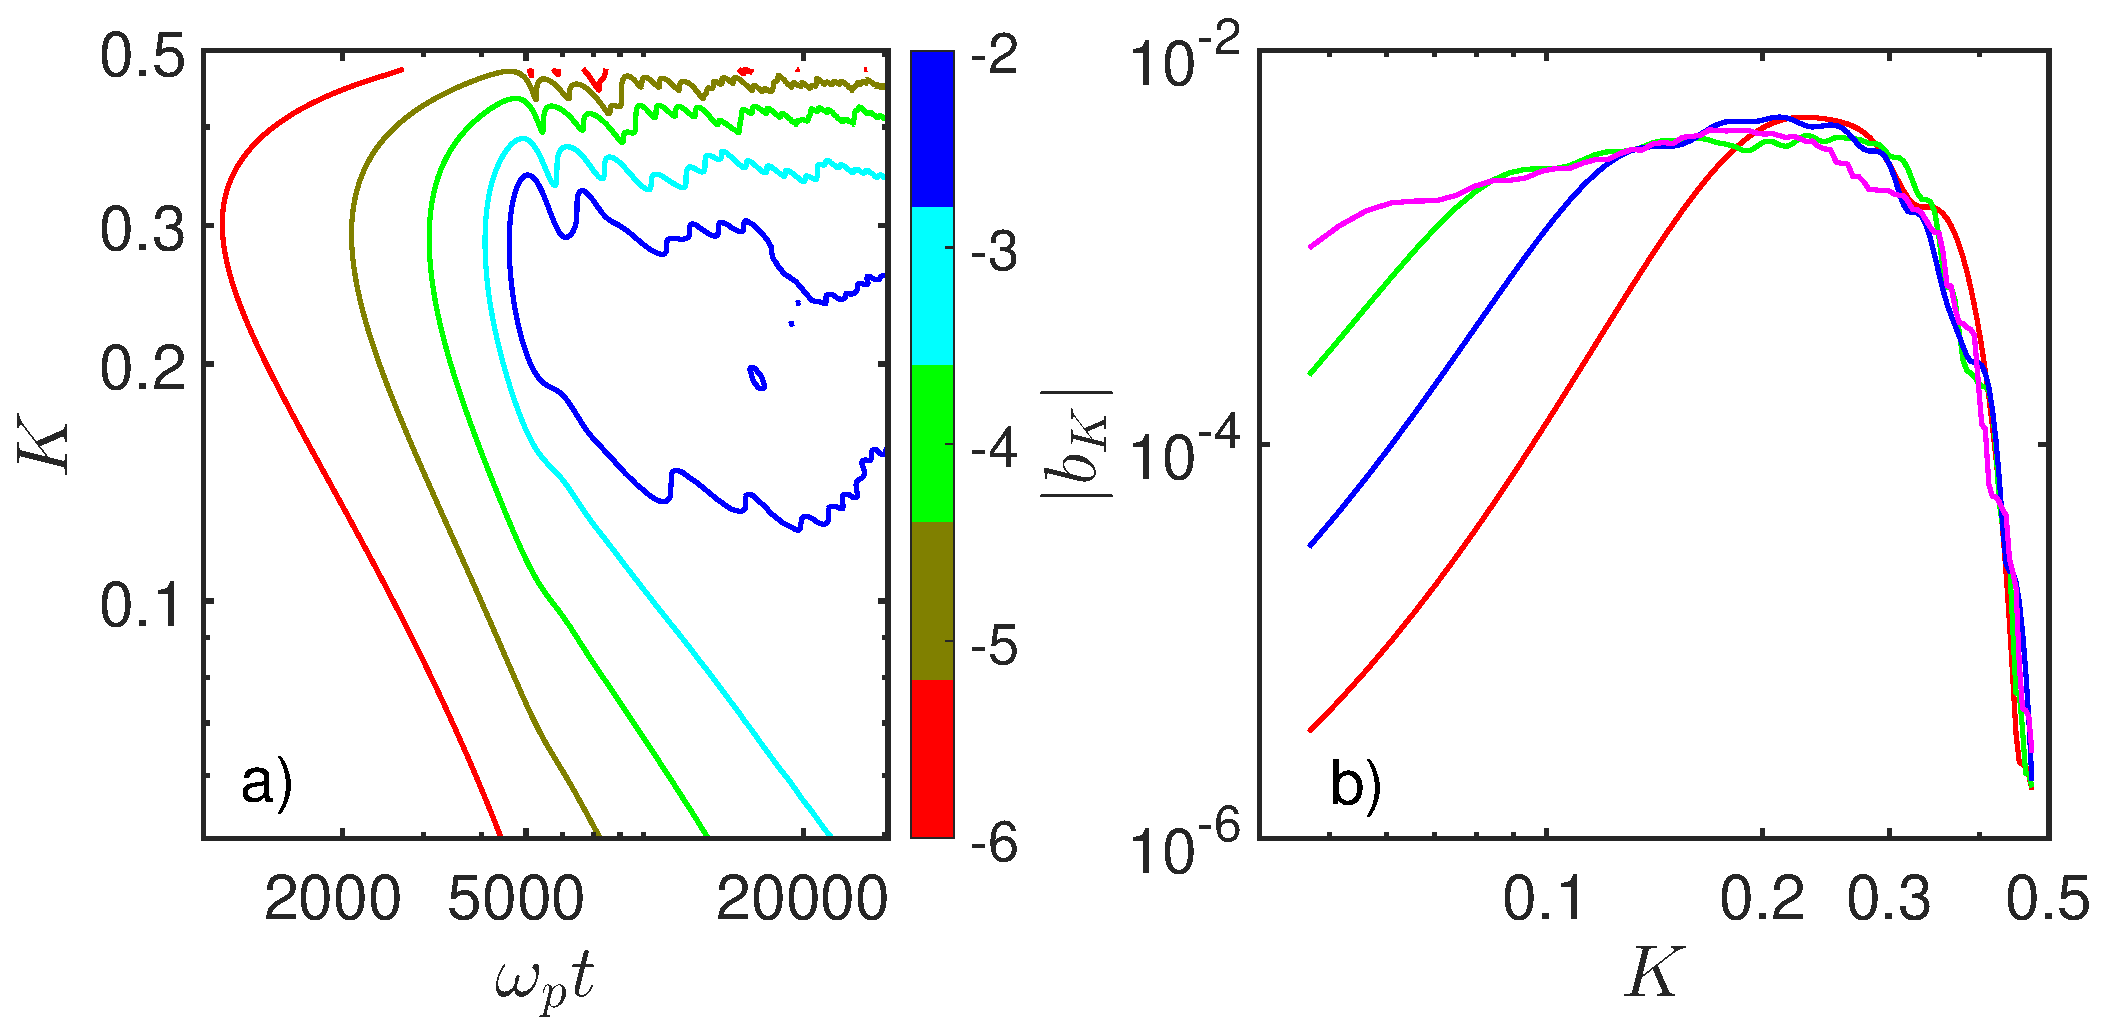
\includegraphics[width=0.9\linewidth]{part1/fig6.eps}
\caption{Эволюция спектра турбулентности, найденная в 1-мерном квазилинейном расчете, в двойном логарифмическом масштабе: (a)~линии уровня логарифма амплитуд мод магнитного поля $|b_K|$; 
(b)~спектр $|b_K|$ магнитного поля в моменты времени $\wpl t$, равные 6000 (красный цвет), 10000 (синий), 16000 (зеленый), 24000 (розовый). Начальная анизотропия $A_0=0.25$.}
\label{fig:dinspectrA025_1d}
\end{figure}

\begin{figure}[t]
\centering
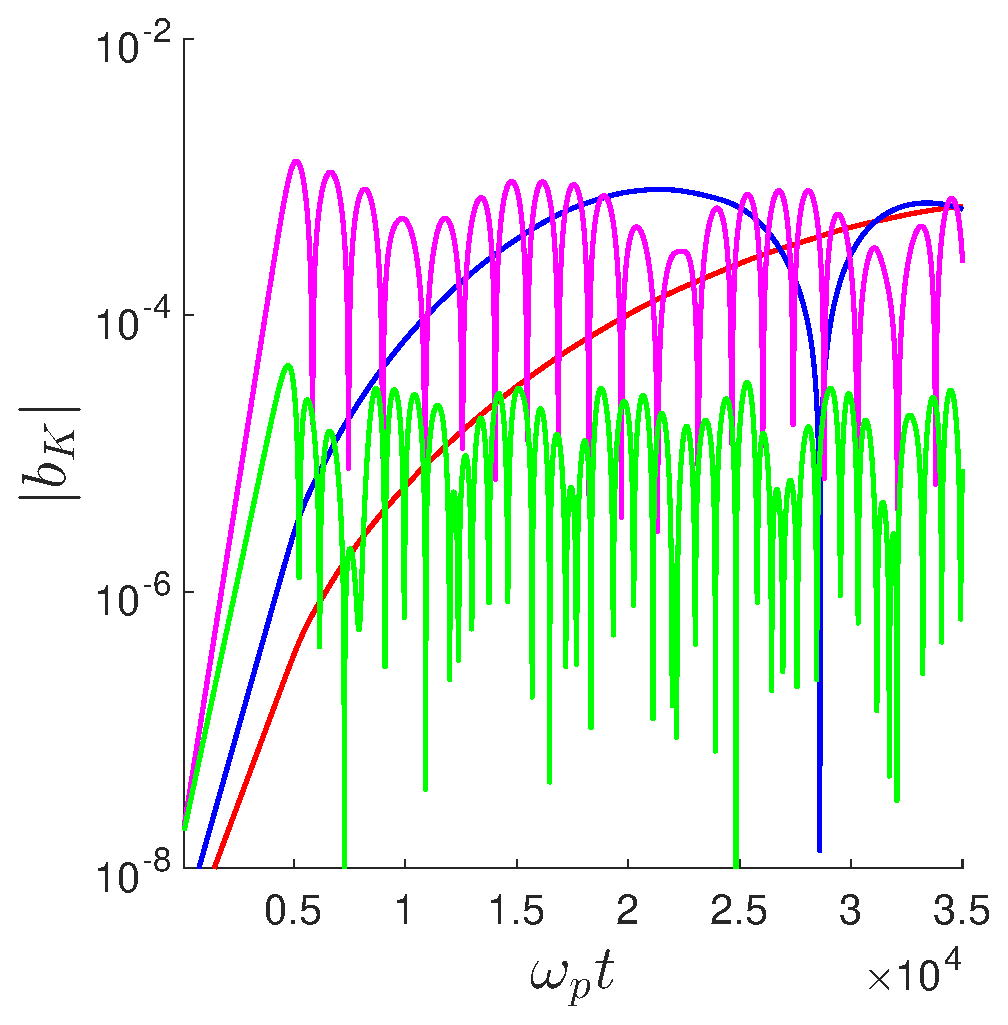
\includegraphics[width=0.65\linewidth]{part1/fig7.eps}
\caption{Эволюция четырех типичных мод ($K=0.08$ --- красный цвет, $K=0.11$ --- синий, $K=0.3$ --- розовый, $K=0.4$ --- зелёный), взятых из спектра рис. \ref{fig:dinspectrA025_1d}. Оптимальное волновое число $K_\mathrm{opt}\approx0.28$.}
\label{fig:evol_garmA025_1d}
\end{figure}

Типичные эволюция всего спектра и динамика отдельных мод на временах порядка десяти времен достижения насыщения наиболее неустойчивой моды с волновым числом $K_\mathrm{opt}\approx0.28$ показаны на рис. \ref{fig:dinspectrA025_1d} и \ref{fig:evol_garmA025_1d}. Для определенности в квазилинейном моделировании в качестве начального использовался равномерный спектр мод с заданной малой амплитудой. Чем она ниже, тем сильнее в ходе первоначального экспоненциального роста спектр сужается около моды с волновым числом $K_\mathrm{opt}$, приобретая колоколообразный вид функции Гаусса. Доминирующие моды с близкими волновыми числами, формирующиеся к моменту насыщения, вступают в квазилинейное взаимодействие и деформируют центральную часть функции распределения, ограничивая свой рост и рост коротковолновых мод, но позволяя расти более длинноволновым модам. Коротковолновое крыло спектра, которое лежит справа от моды с волновым числом $K_{max}$, обладающей наибольшей амплитудой магнитного поля, имеет довольно сложную форму, но в целом допускает крутую степенную аппроксимацию.

Значительная часть длинноволнового крыла спектра, которая примыкает к плато, образованному насытившими свой рост модами, на протяжении длительного промежутка нелинейной эволюции хорошо аппроксимируется степенной зависимостью с показателем, примерно равным 5 и мало меняющимся со временем; см. рис. \ref{fig:dinspectrA025_1d}b. Это обстоятельство дает основание для гипотезы о частичной автомодельности процесса. После насыщения неустойчивости среднее волновое число спектра $\langle K\rangle$ понемногу смещается в длинноволновую сторону. Одновременно с этим немного растет и дисперсия спектра $\sigma^2=\langle K^2\rangle-\langle K\rangle^2$ (см. (\ref{eq:angles})), которая снижалась на линейной стадии развития неустойчивости. Возможная связь указанной эволюции спектра с формированием или разрушением долгоживущих токовых слоев в одномерной вейбелевской турбулентности еще не изучалась.

На рис.~\ref{fig:evol_garmA025_1d} представлена характерная эволюция амплитуд мод с учетом их квазипериодических осцилляций (которые замываются при сложении мод и не видны при визуализации спектра на рис. \ref{fig:dinspectrA025_1d}, где проведено усреднение по близким модам). Пока мода с наибольшим инкрементом не достигнет насыщения, остальные моды растут экспоненциально со своими (разными) инкрементами и не испытывают осцилляций. После этого момента времени моды вблизи оптимальной и более коротковолновые моды тоже практически сразу насыщаются и начинают довольно быстро колебаться, почти не меняя своей амплитуды, т.е. у них величина инкремента значительно ниже появившейся действительной частоты. Вместе с тем более длинноволновые моды с инкрементом значительно меньше максимального продолжают нарастать, правда, почти по степенному закону с различными показателями порядка 3--5, достигают амплитуды порядка максимальной амплитуды моды с оптимальным волновым числом $K_\mathrm{opt}\approx0.28$ и только после этого начинают медленно осциллировать с почти не уменьшающимся уровнем огибающей. Такая динамика мод согласована с указанной выше эволюцией их полного спектра, имеющей автомодельные черты.

Согласно даваемой аналитической теорией~\cite{Pokhotelov2011} оценке уровня насыщения эволюционного параметра $h$ в зависимости от начального параметра анизотропии, нетрудно оценить средний квадрат нормированного насыщающего магнитного поля (см.~(\ref{eq19plus1})), если учесть, что в момент насыщения неустойчивости в спектре доминируют моды с волновыми числами вблизи оптимального $K_\mathrm{opt}$, отвечающего наибольшему линейному инкременту:
\begin{equation}
\label{eq:analit_estimation}
b_{sat}^2\approx0.3\dfrac{A_0^5}{(1+A_0)^6} .
\end{equation}

Полученная оценка соответствует значениям насыщающего магнитного поля, найденным в одномерной задаче в рамках осуществленных нами квазилинейных расчетов, и дает его резкое спадание по закону $\approx 0.3 A_0^5$ при уменьшении начального параметра анизотропии~(рис.~\ref{fig:bsat}a). Для начальных параметров анизотропии больше единицы данная аналитическая оценка не применима, а численное моделирование показывает, что средний квадрат нормированного насыщающего поля с ростом параметра анизотропии стремится к величине чуть меньшей $0.1$~(рис. \ref{fig:bsat}b). При этом, как будет ясно из следующего подраздела, эволюция спектра одномерной турбулентности существенно изменяется. Кроме того, следует заметить, что в более реальном случае двумерной турбулентности, согласно рис. \ref{fig:bsat}b и разделу 4, не только меняется характер спектральной эволюции турбулентности, но и сама зависимость насыщающего магнитного поля от начального параметра анизотропии оказывается существенно другой, сильно отличающейся от~(\ref{eq:analit_estimation}) в сторону увеличения при малых $A_0$ и по-другому выходящей к максимальному значению при больших $A_0$; см., например,~\cite{Borodachev2010,Kuznetsov2022}. 

\begin{figure}[t]
\centering
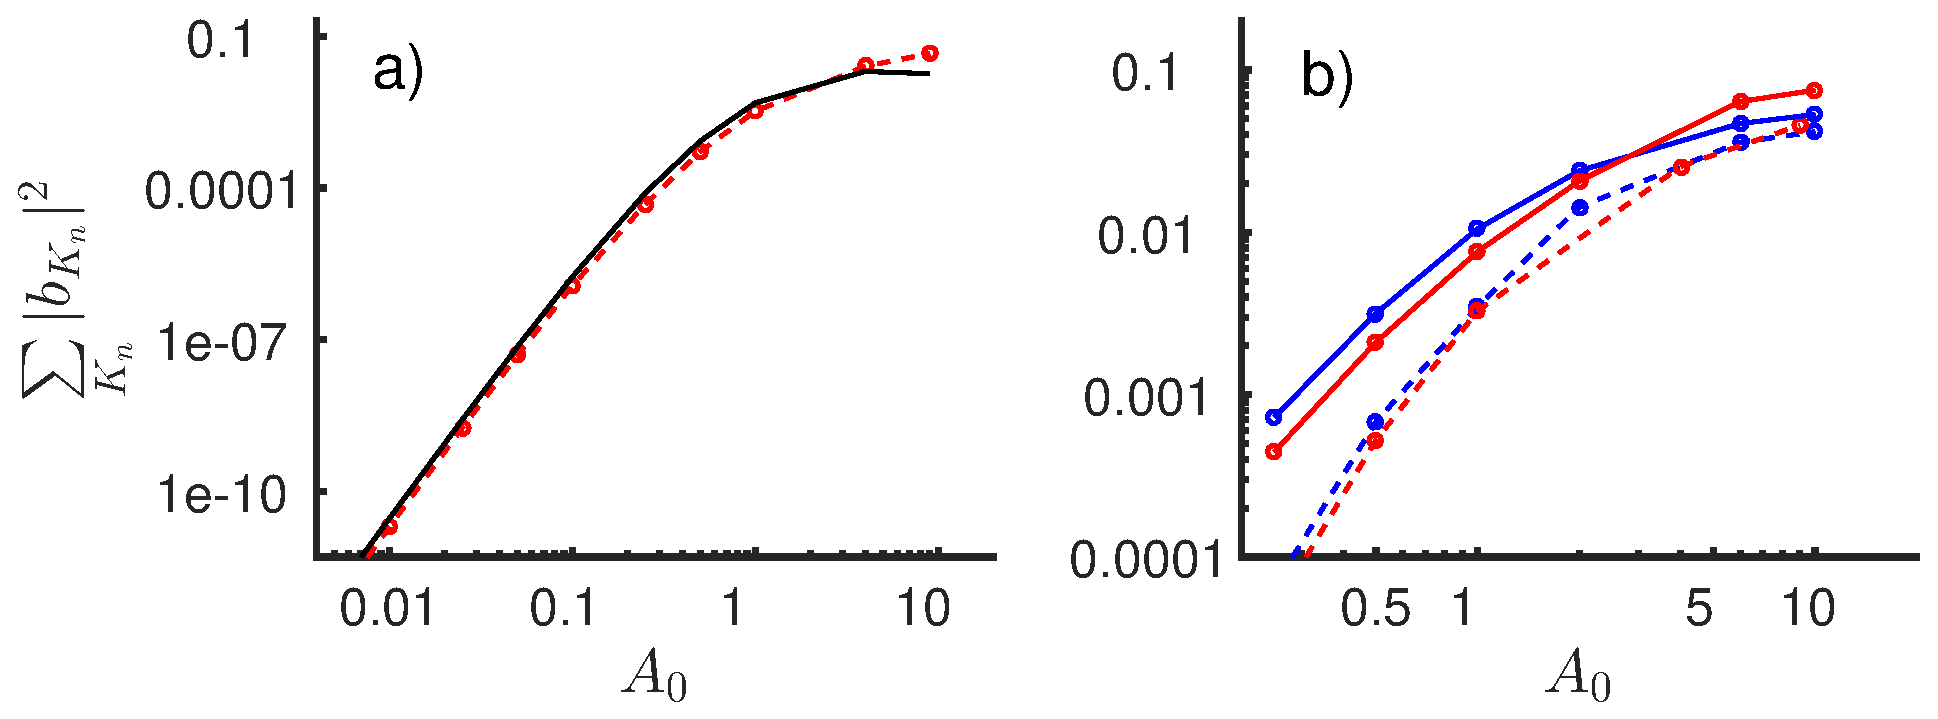
\includegraphics[width=0.9\linewidth]{part1/fig8.eps}
\caption{Сравнение зависимостей среднего квадрата нормированного насыщающего магнитного поля $b_{sat}^2$ от начального параметра анизотропии $A_0$ (a) согласно оценке~(\ref{eq:analit_estimation}) (черный цвет) и численному квазилинейному моделированию по уравнениям (\ref{eq:f0.3})--(\ref{eq:max_eq}) (красный цвет); (b) согласно этому же моделированию (красный цвет) и расчетам методом частиц в ячейках с помощью кода EPOCH (синий цвет) в одномерном (штрихи) и двумерном (сплошная) случаях.}
\label{fig:bsat}
\end{figure}


\subsection{Высокая начальная анизотропия}\label{subsec:high_A_1d}

Если начальная анизотропия велика, $A_0\gg 1$, то исходные инкременты мод тоже велики, турбулентность развивается быстро и сразу в более широком интервале волновых чисел (вблизи оптимальной величины $K_\mathrm{opt}$ и существенно левее нее). На стадии насыщения роста этих мод функция распределения частиц значительно деформируется (в два и более раз) во всей области скоростей порядка тепловых, а не только вблизи своего максимума, как при $A_0\ll 1$. 
\begin{figure}[b]
\centering
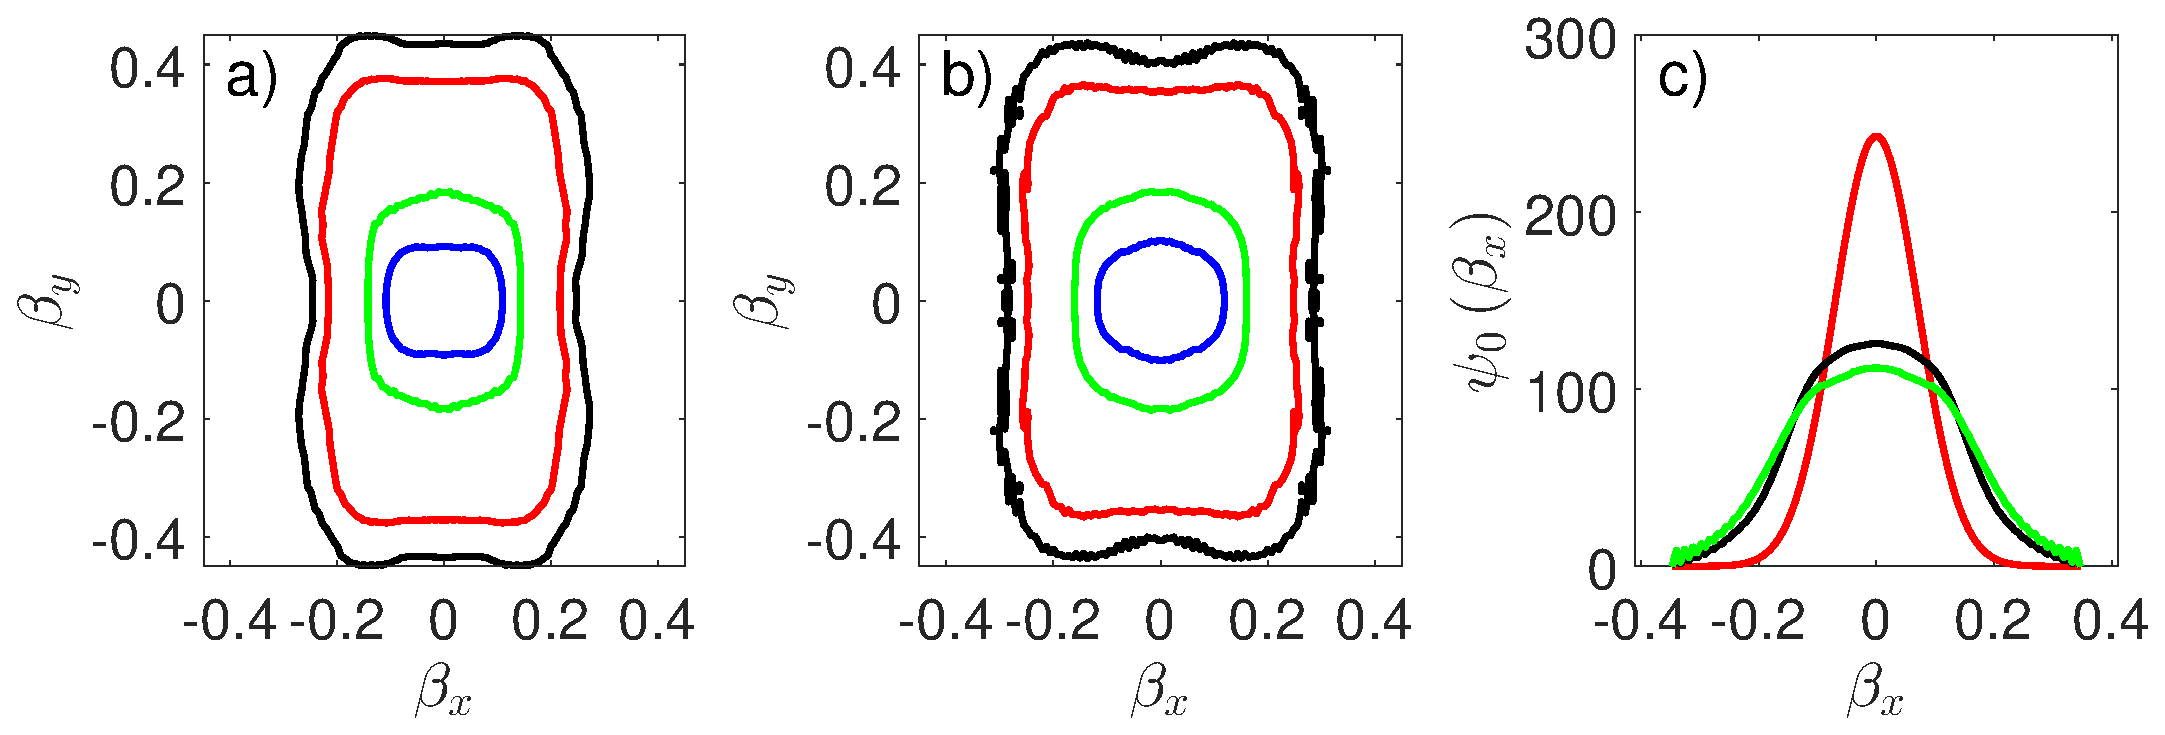
\includegraphics[width=0.85\linewidth]{part1/fig9.eps}
\caption{(a)~Линии уровня $0.05$ (черный цвет), $0.1$ (красный), $0.5$ (зелёный) и $0.8$ (синий), отсчитанные от максимального значения функции распределения в момент времени $\wpl t =80$; (b)~то же в момент времени $\wpl t =440$; (c)~распределение частиц по величине нормированной компоненты скорости $\beta_x$, ортогональной оси анизотропии, в моменты времени $\wpl t$, равные 0 (красный цвет), 80 (черный) и 440 (зеленый). Приведены данные 1-мерного квазилинейного расчета при $A_0=10$.}
\label{fig:sravnenie_FR1d_A10}
\end{figure}
\begin{figure}[b]
\centering
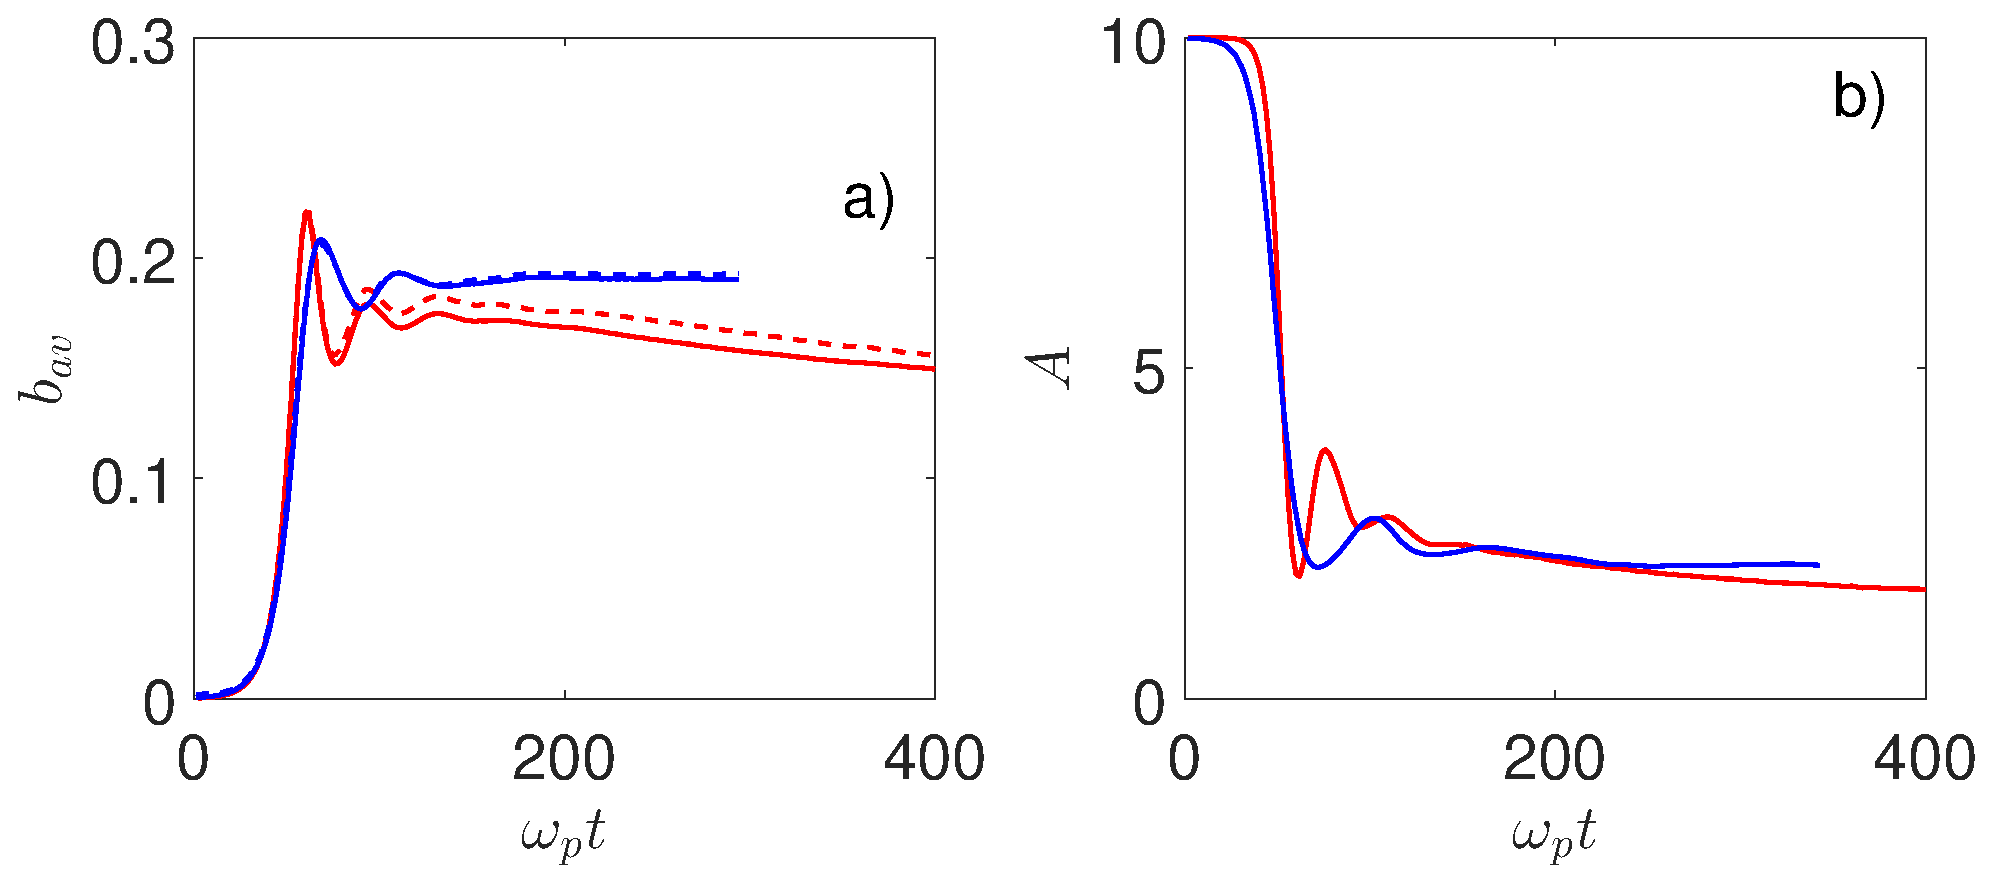
\includegraphics[width=0.8\linewidth]{part1/fig10.eps}
\caption{Эволюция (a) среднеквадратичного магнитного поля $b_{av}$ (сплошная линия) и оценки этой величины~(\ref{eq:otsenka})~(штрихи), а также (b) параметра анизотропии $A$ согласно численному квазилинейному моделированию (красный цвет) и расчетам методом частиц в ячейках (синий цвет) в 1-мерной задаче при $A_0=10$.}
\label{fig:evol1d_QL_A10}
\end{figure}

Согласно нашим расчетам, проведенным для определенности при $A_0=10$ (см. рис. \ref{fig:sravnenie_FR1d_A10} и ср. рис.~\ref{fig:sravnenie_FR1d}), в данном процессе происходит быстрое увеличение поперечной к оси анизотропии скорости электронов, двигавшихся сначала преимущественно вдоль этой оси, так что центральная часть распределения в значительной мере переходит на периферию и его форма вместо овальной приобретает прямоугольный вид с характерным отношением сторон порядка текущего значения параметра анизотропии $A$ после этапа насыщения. Это значение в несколько раз меньше исходного $A_0$, в рассмотренном примере - приблизительно в 5 раз, и в дальнейшем почти не уменьшается ($A\approx 2$, см. рис. \ref{fig:evol1d_QL_A10}). Практически не меняется и форма функции распределения частиц, остающаяся сильно отличной от бимаксвелловской, а также среднеквадратичная величина магнитного поля турбулентности. (Небольшие различия в слабом изменении среднеквадратичного поля $b_{av}$ после достижения им максимума, обнаруживаемые, с одной стороны, квазилинейным расчетом и, с другой стороны, при помощи кода EPOCH, обусловлены, по-видимому, неучтенными нелинейными эффектами в первом и численными шумами, искажающими и тормозящими эволюцию спектра, во втором.) Указанные обстоятельства наряду с обсуждающимся ниже автомодельным характером эволюционирующего спектра одномерной турбулентности опять неявно подтверждают гипотезу о существовании долгоживущих токовых слоев, выявление которых было бы весьма желательно. 

Сравнивая эволюцию спектров турбулентности при высокой (рис.~\ref{fig:dinspectrA10_1d}) и низкой (рис.~\ref{fig:dinspectrA025_1d}) начальной анизотропии, заметим, что в первом случае затухание насытившихся, более коротковолновых мод оказывается значительно сильнее и автомодельный характер эволюции обоих крыльев спектра выражен более явно, чем во втором. Поэтому в случае высокой начальной анизотропии дисперсия спектра $\sigma^2=\langle K^2\rangle-\langle K\rangle^2$ заметно изменялась (уменьшалась) только на стадии экспоненциального роста мод, а после кратковременного уширения с началом нелинейной стадии уменьшается очень слабо, стремясь к постоянному значению, в отличие от случая низкой начальной анизотропии, когда эта дисперсия после первоначального уменьшения на линейной стадии медленно увеличивается за счет нелинейного (квазилинейного) роста длинноволнового крыла спектра. При этом среднее волновое число спектра $\langle K\rangle$ в первом случае со временем уменьшается примерно по степенному закону $t^{-1/2}$, тогда как во втором оно уменьшается весьма незначительно. Наконец, в первом случае, при $A_0=10$, близкий к степенному вид обоих крыльев спектра $|b_{k}|$ прослеживается гораздо более четко и практически сразу после насыщения роста среднеквадратичного поля, характеризуясь почти не меняющимися показателями около 10 и -13 в длинноволновой и коротковолновой частях соответственно, хотя эти показатели весьма чувствительны к начальному уровню амплитуд мод. Заметим, что во втором случае, при $A_0=0.25$, степенной вид принимает только длинноволновое крыло, причем с показателем примерно вдвое меньшем, т.е. около 5, и тоже чувствительным к начальному уровню амплитуд мод.
\begin{figure}[t]
\centering
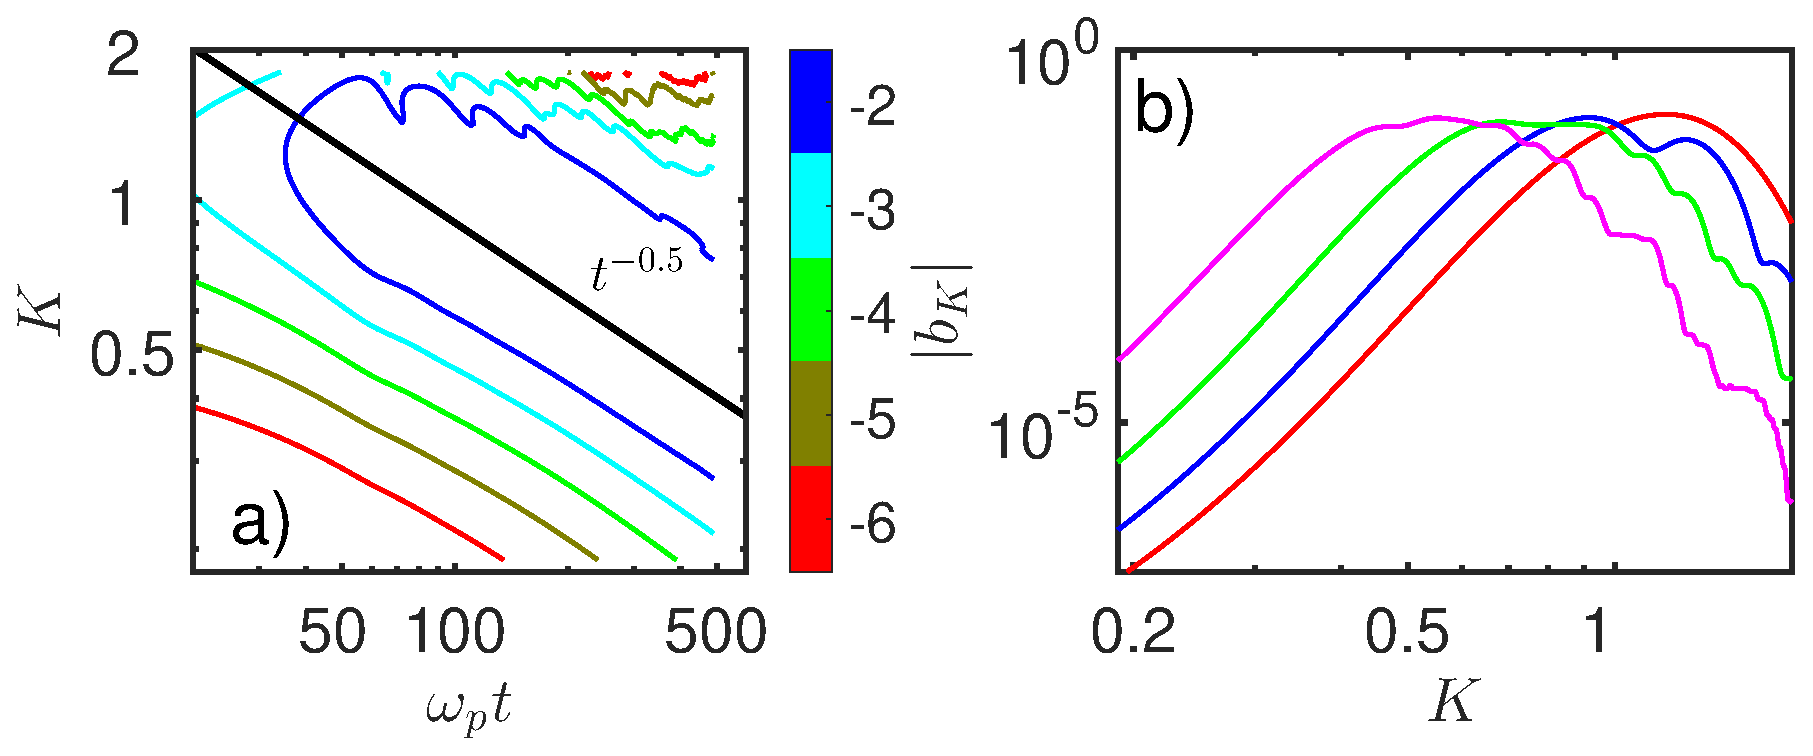
\includegraphics[width=0.8\linewidth]{part1/fig11.eps}
\caption{Эволюция спектра турбулентности, найденная в 1-мерном квазилинейном расчете, в двойном логарифмическом масштабе: (a)~линии уровня логарифма амплитуд мод магнитного поля $|b_K|$; (b)~спектр $|b_K|$ магнитного поля в моменты времени $\wpl t$, равные 60 (красный цвет), 100 (синий), 180 (зеленый) и 360 (розовый). Начальная анизотропия $A_0=10$.}
\label{fig:dinspectrA10_1d}
\end{figure}

\begin{figure}[b]
\centering
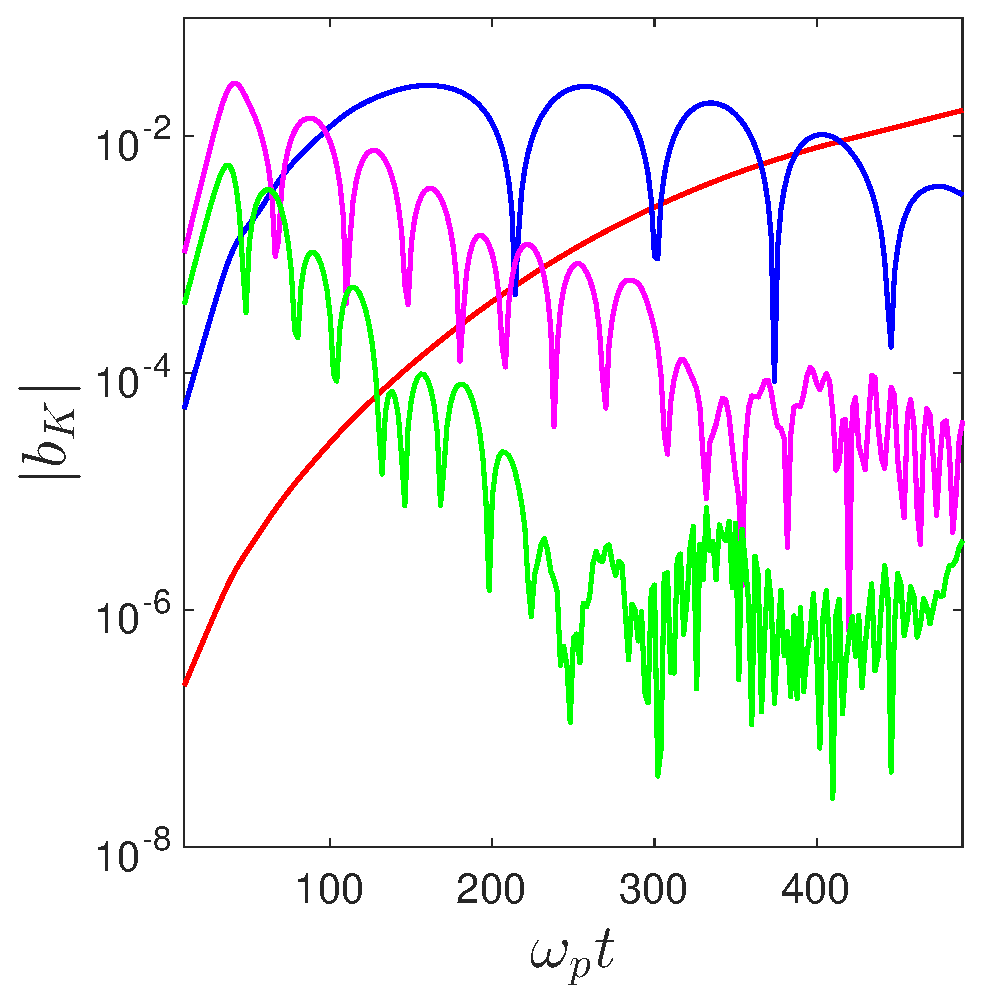
\includegraphics[width=0.5\linewidth]{part1/fig12.eps}
\caption{Эволюция четырех типичных мод ($K=0.4$ --- красный цвет, $K=0.7$ --- синий, $K=1.2$ --- розовый, $K=1.6$ --- зелёный), взятых из спектра рис. \ref{fig:dinspectrA10_1d}. Оптимальное волновое число $K_\mathrm{opt}\approx1.2$.}
\label{fig:evol_garmA010_1d}
\end{figure}

Для сформировавшейся сложно анизотропной функции распределения
большинство мод приобретают действительную частоту больше или порядка величины инкремента (декремента), а следовательно, их амплитуды $|b_{k}|$ начинают осциллировать, что отмечалось в предыдущем подразделе при $A_0=0.25$. Теперь, при $A_0=10$, это показано на рис.~\ref{fig:evol_garmA010_1d}, где частота осцилляций выше у более коротковолновых мод, причем для менее коротковолновых мод имеется промежуточная стадия примерно степенного роста (с различными показателями степени, опять, порядка 3-5, как и при $A_0=0.25$), начинающаяся почти сразу после момента насыщения моды с наибольшим исходным инкрементом и оптимальным волновым числом $K_\mathrm{opt}\approx1.2$ и заканчивающаяся моментом их собственного насыщения, после которого и возникают указанные осцилляции их амплитуд. Дальнейшее затухание огибающих этих осциллирующих амплитуд теперь выражено весьма сильно и является примерно экспоненциальным, а не степенным. Оно идет с разными декрементами в диапазоне 0.01-0.05 для различных мод, опускающихся вплоть до уровня численных шумов порядка $10^{-5}$. Осцилляции не наблюдаются только для наиболее длинноволновых мод, дисперсия которых, по-видимому, определяется уплощенной частью функции распределения, а их действительные частоты могут быть даже меньше их инкрементов (декрементов).

Согласно проведенному нами сравнительному анализу расчетов в рамках квазилинейного подхода и расчетов методом частиц в ячейках для указанных и других значений параметра анизотропии $A_0$, подобная динамика отдельных мод и спектра в целом в одномерной задаче обусловлена в основном чисто квазилинейными эффектами благодаря продолжающей самосогласованно изменяться функции распределения частиц. Тем не менее, из-за наличия уже упоминавшихся значительных численных шумов в использованном коде EPOCH, искажающих форму функции распределения и квазилинейную динамику мод, открытым остается вопрос о количественной оценке возможной, пусть малой, роли четырехволнового взаимодействия в нарастании все более длинноволновых и затухании ранее возбудившихся коротковолновых мод, а следовательно, в формировании и поддержании степенной формы крыльев спектра одномерной вейбелевской турбулентности, особенно на поздних этапах ее затухания.           % Глава 1
\chapter{Развитие двумерной аксиально симметричной турбулентности}\label{ch:ch2}

\section{Вывод системы квазилинейных уравнений}\label{sec:ch2/sec1}

Поставленный вопрос и выяснение других качественных особенностей эволюции вейбелевской турбулентности, квазилинейных и не только, являются также актуальными для более реалистичной двумерной (2D3V) задачи, которая рассматривается в настоящем разделе и для которой расчеты кодом EPOCH являются более точными, поскольку его численные шумы не так сильно искажают функцию распределения частиц и динамику мод, как в одномерной задаче. Для определенности анализ ограничен простейшим аксиально симметричным случаем, в котором ось анизотропии $y$ исходного бимаксвелловского распределения электронов по скоростям (\ref{bimax}) ортогональна расчетной плоскости $xz$. В этом случае TEM-турбулентности, как будет ясно из дальнейшего, квазилинейные эффекты тоже доминируют и определяют основные свойства ее пространственного спектра. Последний для интересующих нас полей и токов представляется большим числом $s \cdot p$ неколлинеарных мод (гармоник) с волновыми векторами $\{ (k_{1}; k_{1}),\, (k_{1}; k_{2}),...,\, (k_{2}; k_{1}),...\, (k_{s}; k_{p}) \}$, компоненты которых состоят из $s$ радиальных проекций $\vec{k}\vec{r}_0$ и $p$ аксиальных проекций $\vec{k}\vec{\phi}_0$. В таком представлении обе компоненты магнитного поля, которое ортогонально оси анизотропии, имеют вид суммы мод по целочисленному векторному индексу $\vec{n}=(n_r,n_\phi)$:
\begin{align}
B_{x,z}(t,x,z) = \mathrm{Re} \sum^{l,p}_{n_r,n_\phi=1}\left(B_{k_{\vec{n}}}(t)\right)_{x,z}\exp(- \mathrm{i}\left(k_{\vec{n}}\right)_x x - \mathrm{i}\left(k_{\vec{n}}\right)_z z).
\end{align}
Аналогичен вид и единственной компоненты электрического поля $\vec{E}=(0, E_y, 0)$, направленного вдоль оси анизотропии функции распределения и ниже нормированного так же, как магнитное поле 
(\ref{eq19plus2}).

%систему (\ref{eq:f0.4})--(\ref{eq:maxw3.3}) с оператором (\ref{eq:oper.4})

Для указанных мод полей и возмущений-гармоник функции распределения электронов по скоростям получаем следующую систему квазилинейных уравнений с новым более сложным оператором $\hat \Theta_1$ вместо оператора $\hat \Phi$ одномерной задачи (ср. (\ref{eq:f0.3})--(\ref{eq:max_eq}), (\ref{eq:oper.2})): 
% \begin{wide}
\begin{align}
\label{eq:f0.4}
\dfrac{\partial \psi_0}{\partial \tau}+\sum\limits^{m}_{n=1}\mathrm{Re}\Bigg[\hat \Theta_1\left(e_{\vec{K}_{\vec{n}}},{\vec{b}}_{\vec{K}_{\vec{n}}},\psi_{K_n}^*\right)\Bigg]=0,\\
% \end{align}
% \begin{align}
\label{eq:f1.4}\dfrac{\partial \psi_{K_n}}{\partial \tau}+\mathrm{i}\left(K_{\vec{n}}\right)_x\beta_x\psi_{K_n}+\mathrm{i}\left(K_{\vec{n}}\right)_z\beta_z\psi_{K_n}+2\hat \Theta_1\left(e_{\vec{K}_{\vec{n}}},{\vec{b}}_{\vec{K}_{\vec{n}}},\psi_{0}\right)+\hat \Theta_1\left(e_{\vec{K}_{\vec{n}}}^*,{\vec{b}}_{\vec{K}_{\vec{n}}}^*,\psi_{2K_n}\right)=0,\\
% \end{align}
% \begin{align}
\label{eq:f2.4}
\dfrac{\partial \psi_{2K_n}}{\partial \tau}+2\mathrm{i}\left(K_{\vec{n}}\right)_x\beta_x\psi_{2K_n}+2\mathrm{i}\left(K_{\vec{n}}\right)_z\beta_z\psi_{2K_n}+\hat \Theta_1\left(e_{\vec{K}_{\vec{n}}},{\vec{b}}_{\vec{K}_{\vec{n}}},\psi_{K_n}\right)=0,\\
% \end{align}
% \begin{align}   
    \dfrac{\partial \left({b}_{\vec{K}_{\vec{n}}}\right)_z}{\partial \tau}=-\mathrm{i}\left(K_{\vec{n}}\right)_xe_{\vec{K}_{\vec{n}}},\quad 
    \dfrac{\partial \left({b}_{\vec{K}_{\vec{n}}}\right)_x}{\partial \tau}=\mathrm{i}\left(K_{\vec{n}}\right)_ze_{\vec{K}_{\vec{n}}}, \\
\label{eq:maxw3.3}
    \dfrac{\partial e_{\vec{K}_{\vec{n}}}}{\partial \tau}=\mathrm{i}\left({b}_{\vec{K}_{\vec{n}}}\right)_x\left(K_{\vec{n}}\right)_z-\mathrm{i}\left({b}_{\vec{K}_{\vec{n}}}\right)_z\left(K_{\vec{n}}\right)_x+\beta_{\|0}^{-1}{\iiint\limits^{+\infty}_{-\infty}\beta_y\psi_{\vec{K}_{\vec{n}}}(\tau,\beta_x,\beta_y,\beta_z)d\beta_xd\beta_yd\beta_z} ,\\
% \end{align}
% \begin{align}
\label{eq:oper.4}
\hat \Theta_1\left(e_{\vec{K}_{\vec{n}}},{\vec{b}}_{\vec{K}_{\vec{n}}},\psi(\beta)\right)  =  \dfrac{e_{\vec{K}_{\vec{n}}}}{2}\dfrac{\partial \psi(\beta)}{\partial \beta_y}-\dfrac{\left({b}_{\vec{K}_{\vec{n}}}\right)_z}{2} \left(\beta_x\dfrac{\partial \psi(\beta)}{\partial \beta_y}-\beta_y\dfrac{\partial \psi(\beta)}{\partial \beta_x}\right) \nonumber \\
-\dfrac{\left({b}_{\vec{K}_{\vec{n}}}\right)_x}{2} \left(\beta_z\dfrac{\partial \psi(\beta)}{\partial \beta_x}-\beta_x\dfrac{\partial \psi(\beta)}{\partial \beta_z}\right) .
\end{align}
% \end{wide}


\section{Сравнение с результатами моделирования методом частиц в ячейках. Выявление нелинейных эффектов четырехволнового взаимодействия на фоне квазилинейной динамики мод.}\label{sec:ch2/sec1}
Мы исследовали ее двумерно-неоднородные решения, получаемые численно на основе метода Стёрмера~-- Верле (Leapfrog)~\cite{Birdsall2018} (см. конец раздела 2) при одной и той же исходной поперечной тепловой скорости $\beta_{\perp0}=0.1$ и различной начальной анизотропии. Кроме того, опять проводилось сравнение с моделированием методом частиц в ячейках при помощи кода EPOCH, которое в целом оказалось согласованным с квазилинейным моделированием системы (\ref{eq:f0.4})-(\ref{eq:oper.4}) с точностью $\sim10-30\%$. Соответствующие результаты приведены ниже при $A_0=0.25$ и $A_0=10$, как и в предыдущем разделе для одномерной задачи. Отметим, что и для двумерной задачи в предположении об аксиально симметричном и достаточно узком пространственном спектре вейбелевской турбулентности, согласно~\cite{Nechaev2023} и (\ref{eq:otsenka}), нетрудно получить следующее приближенное аналитическое соотношение для эволюционирующих среднеквадратичного магнитного поля $b_{av}$, параметра анизотропии плазмы $A$ (ср. (\ref{eq:A_1d})) и среднего радиального волнового числа (\ref{eq:angles}) $\langle K\rangle$ (ср. начало раздела 3): 
\begin{equation}
\label{eq:otsenka2d}
b_{av}^2 = \frac{A_0-A}{1+A_0}\cdot\dfrac{\langle K\rangle^2}{A \langle K\rangle^2+A+5\langle K\rangle^2+3} ,
\end{equation}
\begin{equation}
\label{eq:A_2d}
A=\frac{2\iiint\limits^{\infty}_{-\infty}\beta_y^2\psi_{0}(\tau,\beta_x,\beta_y,\beta_z) d\beta_x d\beta_yd\beta_y}{\iiint\limits^{\infty}_{-\infty}\left(\beta_x^2+\beta_z^2\right)\psi_{0}(\tau,\beta_x,\beta_y,\beta_z) d\beta_x d\beta_y d\beta_z}-1 .
\end{equation}
Это соотношение для аксиально симметричной (в среднем) турбулентности по-прежнему очень хорошо, с точностью до нескольких процентов, выполнялось в квазилинейных расчетах~(см., например, рис.~\ref{fig:evol2d}a) и немного хуже, с точностью до 10-20\%, в расчетах методом частиц в ячейках, где в условиях высокого уровня численных шумов спектр оказывался более широким. Отметим, что всюду ниже под спектром вейбелевской турбулентности в аксиально симметричной задаче подразумевается зависимость нормированных амплитуд мод магнитного поля (\ref{eq19plus1}) $|b_K|$ от нормированного радиального волнового числа (\ref{eq19plus2}) $K$, получаемая после усреднения по азимутальному углу. 
\begin{figure}[t]
\centering
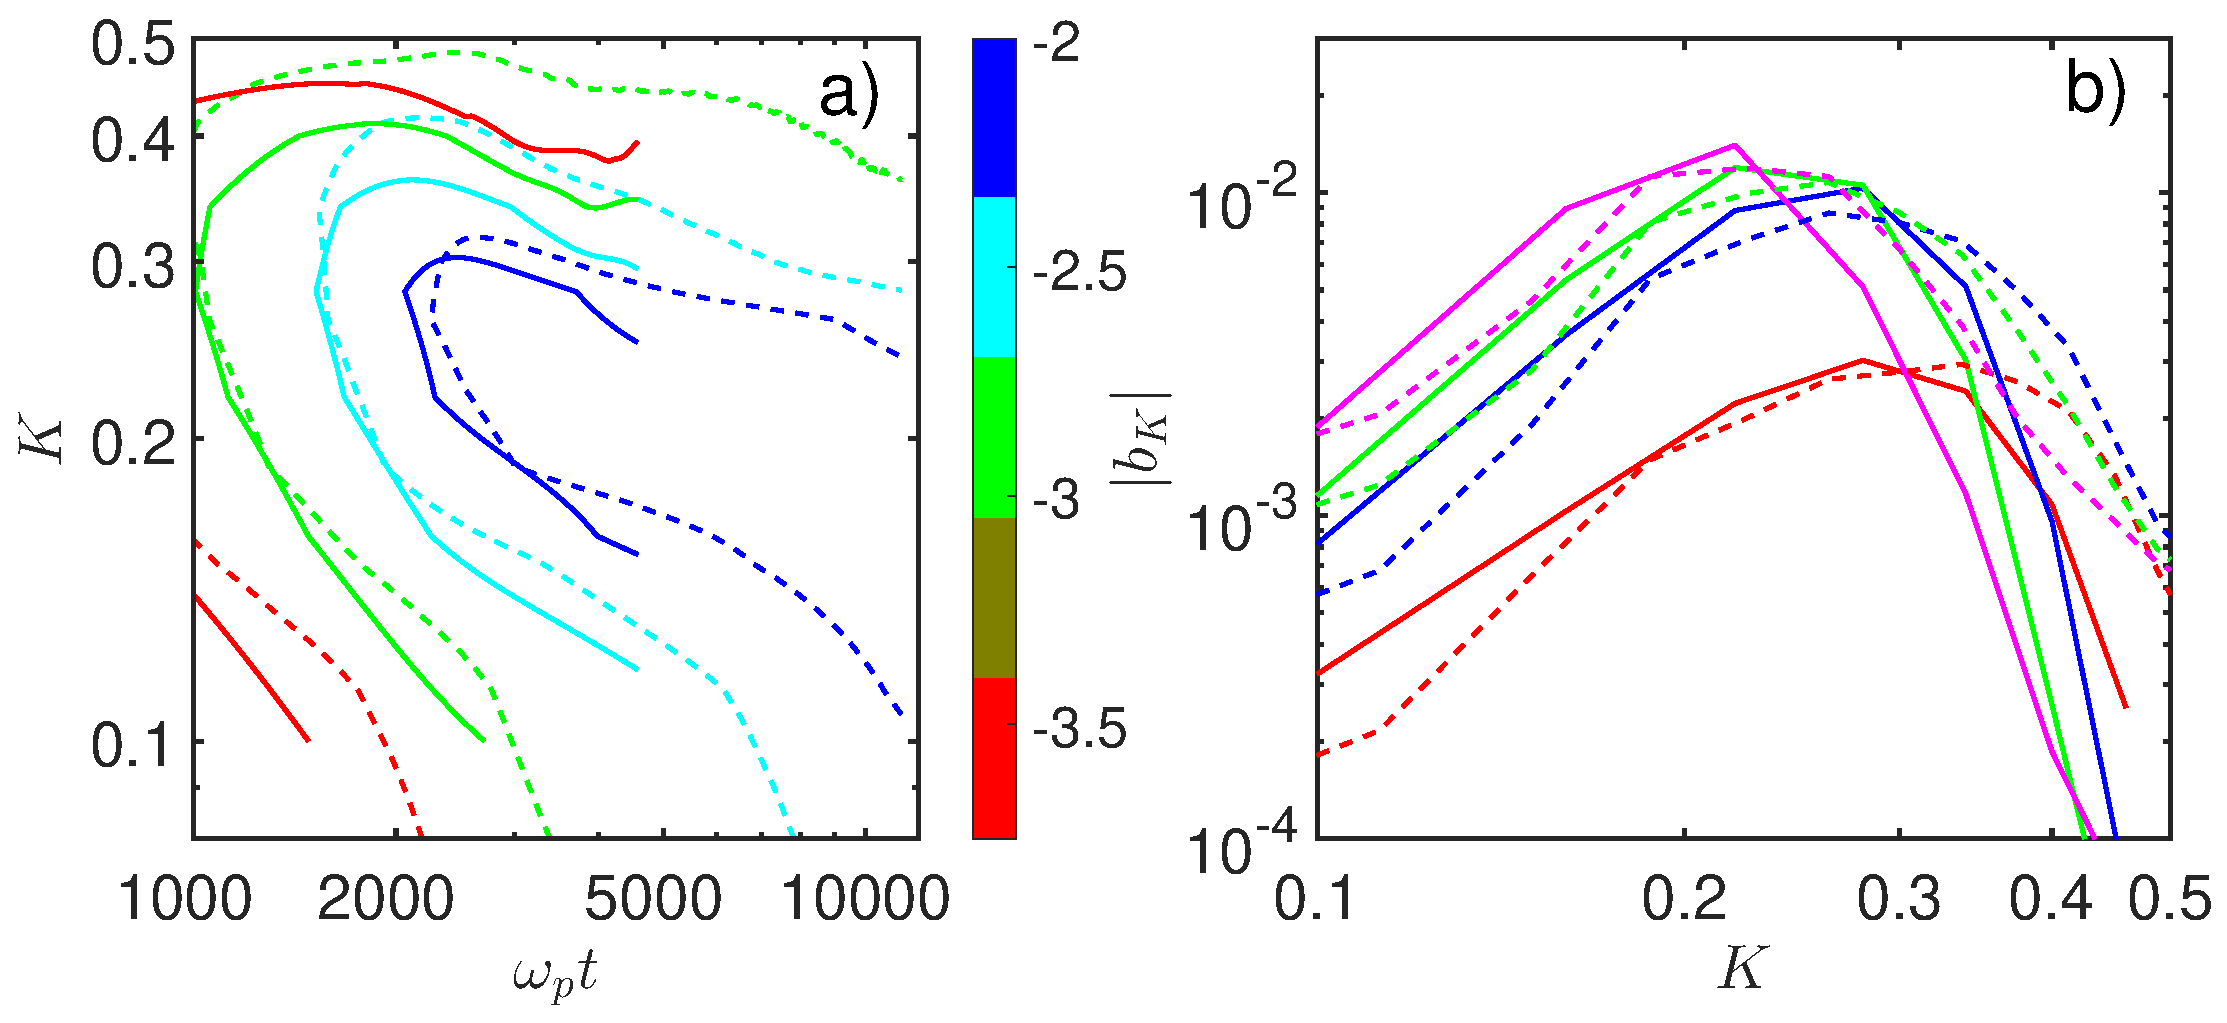
\includegraphics[width=0.9\linewidth]{part2/fig13.eps}
\caption{Эволюция спектра турбулентности, найденная в аксиально симметричных расчетах методом частиц в ячейках (штрихи) и на основе квазилинейного подхода (сплошная линия), в двойном логарифмическом масштабе: (a)~линии уровня логарифма амплитуд мод магнитного поля $|b_K|$; (b)~спектр $|b_K|$ магнитного поля в моменты времени $\wpl t$, равные 1500 (красный цвет), 2400 (синий), 3000 (зеленый) и 4500 (розовый). Начальная анизотропия $A_0=0.25$.
}
\label{fig:dinspectrA025_2d}
\end{figure}


Не повторяя общие положения, сформулированные в подразделах 3.1 и 3.2, сосредоточимся только на различиях в развитии турбулентности, обусловленных переходом от одномерной к двумерной задаче, т.\,е. расширением области волновых векторов неустойчивых мод и направлений их магнитных полей, а следовательно, усилением квазилинейного взаимодействия мод и деформации функции распределения электронов по скоростям.
\begin{figure}[t]
\centering
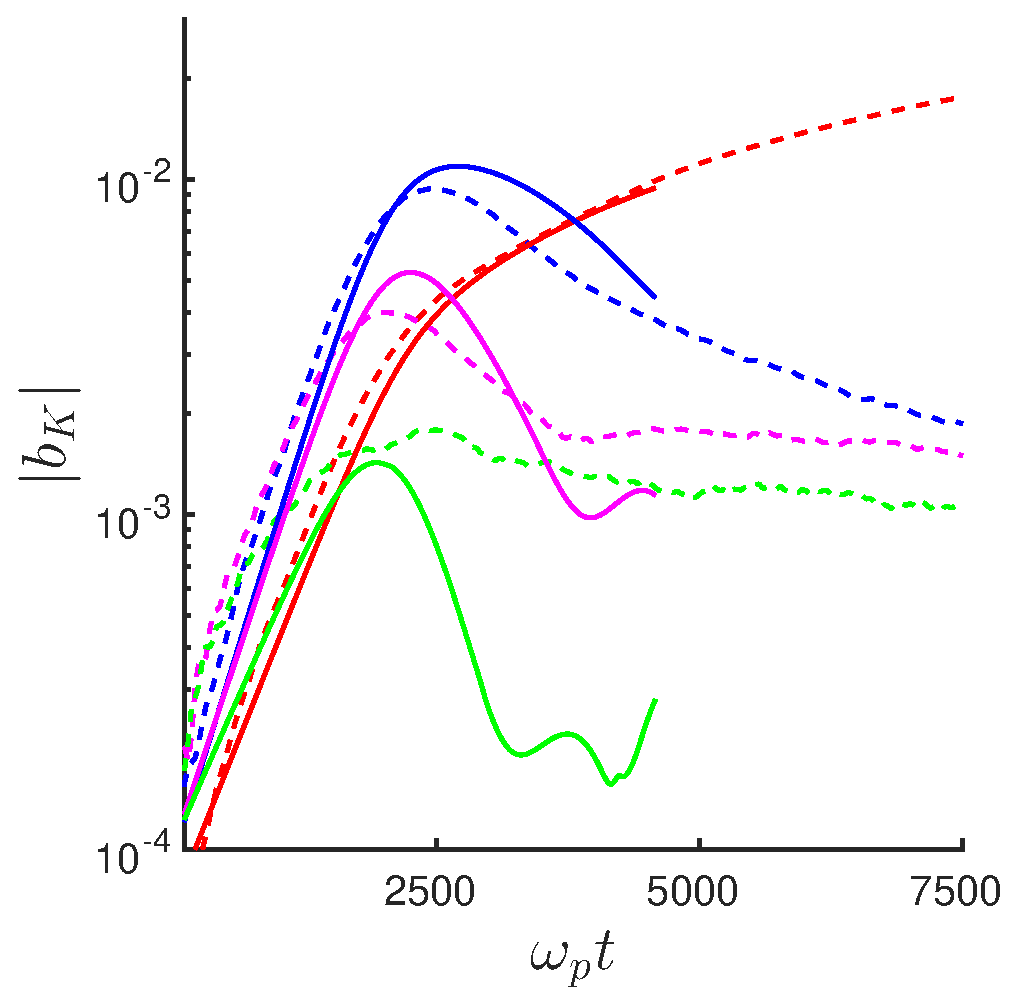
\includegraphics[width=0.5\linewidth]{part2/fig14.eps}
\caption{Эволюция четырех типичных мод ($K=0.16$ --- красный цвет, $K=0.28$ --- синий, $K=0.34$ --- розовый, $K=0.4$ --- зелёный), взятых из спектра рис. \ref{fig:dinspectrA025_2d}. Оптимальное волновое число $K_\mathrm{opt}\approx0.28$.}
\label{fig:evol_garmA025}
\end{figure}

При низкой начальной анизотропии, $A_0=0.25$, деформация функции распределения идет интенсивнее, дольше и по величине составляет уже не доли, а несколько процентов, захватывая более обширную область тепловых скоростей электронов, так что тангенс угла конуса, на котором согласно рис.~\ref{fig:sravnenie_FR1d} меняется знак приращения функции распределения, увеличивается от примерно 1/6 до почти 1/2. При этом в баунс-осцилляциях участвует больше электронов, а функция распределения становится менее анизотропной и по форме ближе к бимаксвелловской, причем величина анизотропии с наступлением нелинейной стадии падает не осциллируя и не на 1-2\% (как было показано на рис.~\ref{fig:evol1d_QL_A025}b), а почти на 20\%, продолжая снижаться в дальнейшем. Значительнее уменьшается, не осциллируя, и среднее волновое число $\langle K\rangle$ энергонесущих мод, а насыщающее среднеквадратичное магнитное поле $b_{sat}$ оказывается сильнее приблизительно в 5 раз и тоже не осциллирует, хотя по-прежнему почти не снижается по величине на рассмотренных временах, в несколько раз превышающих время наступления насыщения. Данные результаты квазилинейного подхода согласуются с предшествующими численными исследованиям вейбелевской неустойчивости методом частиц в ячейках, например,~\cite{Borodachev2010,Borodachev2016_Radiofiz}. 

В рассмотренном типичном примере смещение спектра турбулентности в длинноволновую область, как показано на рис.~\ref{fig:dinspectrA025_2d}, выражено более явно и сопровождается затуханием коротковолновых мод, а не только ростом длинноволновых, что имело место в одномерной задаче (ср. рис.~\ref{fig:dinspectrA025_1d}, где время наступления насыщения почти вдвое больше, поскольку логарифмический уровень начальных амплитуд мод был задан примерно вдвое ниже, чем на рис.~\ref{fig:dinspectrA025_2d}). Такое поведение спектра обусловлено более эффективным квазилинейным, но не четырехволновым взаимодействием мод, что подтверждает аналогичный расчет методом частиц в ячейках, который учитывает оба механизма взаимодействия мод и которому на рисунке отвечают штриховые линии, хорошо совпадающие со сплошными. Благодаря менее анизотропной и более гладкой форме функции распределения, согласованной с двумерной турбулентностью, отдельные моды в ходе ее эволюции остаются по существу апериодическими, т.\,е. их инкременты (декременты) превышают по величине возможные значения действительных частот. Следовательно, в отличие от одномерной турбулентности, квазипериодические осцилляции амплитуд мод практически отсутствуют и их начальный рост с последующим затуханием определяется изменяющейся величиной инкремента, переходящего после насыщения в декремент; ср. рис. \ref{fig:evol_garmA025} и \ref{fig:evol_garmA025_1d}. При этом из-за изменения во времени инкремента (декремента) мод оказывается возможным не строго экспоненциальный, а скорее близкий к степенному как рост их амплитуд на промежуточном этапе эволюции до достижения максимальной величины (который начинается после насыщения наиболее быстро растущей моды с оптимальным волновым числом $K_\mathrm{opt}\approx0.28$), так и дальнейшее затухание. Со временем совместная динамика мод отражается в автомодельных чертах спектра турбулентности $|b_K|$, у которого в представленном примере длинноволновое и коротковолновое крылья неплохо аппроксимируются степенными зависимостями с показателями около 2 и -10 соответственно.
\begin{figure}[t]   
\centering
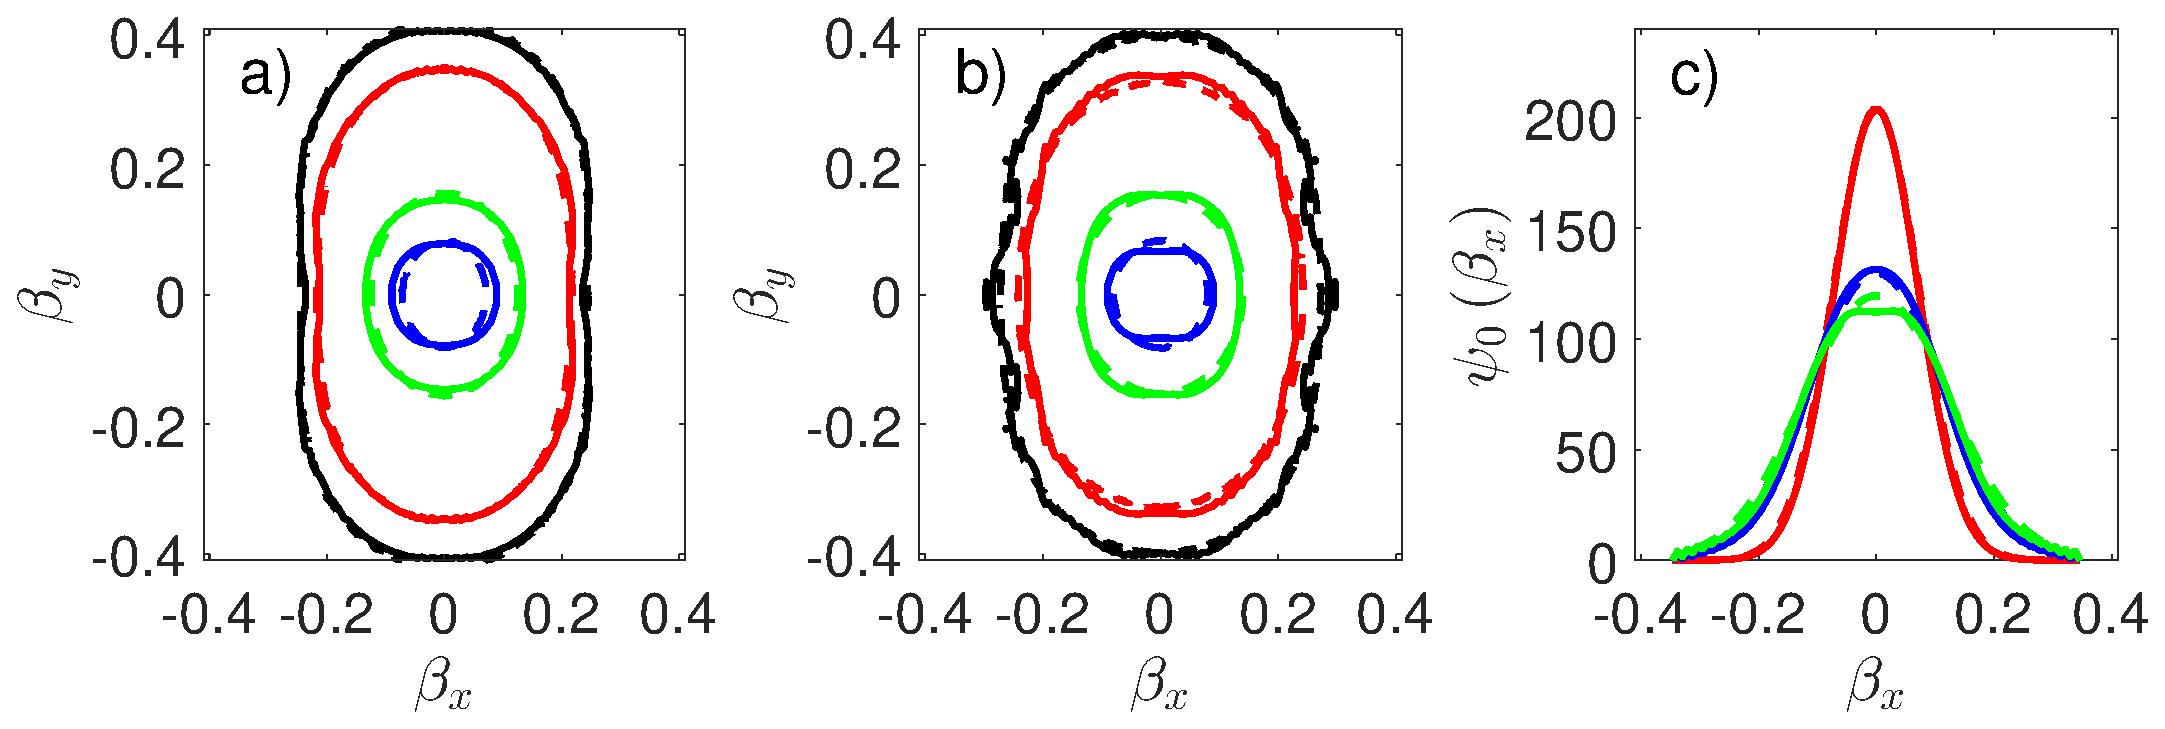
\includegraphics[width=0.9\linewidth]{part2/fig15.eps}
\caption{(a)~Линии уровня $0.05$ (черный цвет), $0.1$ (красный), $0.5$ (зелёный) и $0.8$ (синий), отсчитанные от максимального значения функции распределения в момент времени $\wpl t =83$; (b)~то же в момент времени $\wpl t =170$; (c)~распределение частиц по величине нормированной компоненты скорости $\beta_x$, ортогональной оси анизотропии, в моменты времени $\wpl t$, равные 0 (красный цвет), 83 (синий) и 170 (зеленый). Приведены данные аксиально симметричных расчетов методом частиц в ячейках (штрихи) и в рамках квазилинейного подхода (сплошная) при $A_0=10$.
}
\label{fig:sravnenie_FR2dax_3im}
\end{figure}

\begin{figure}[b]
\centering
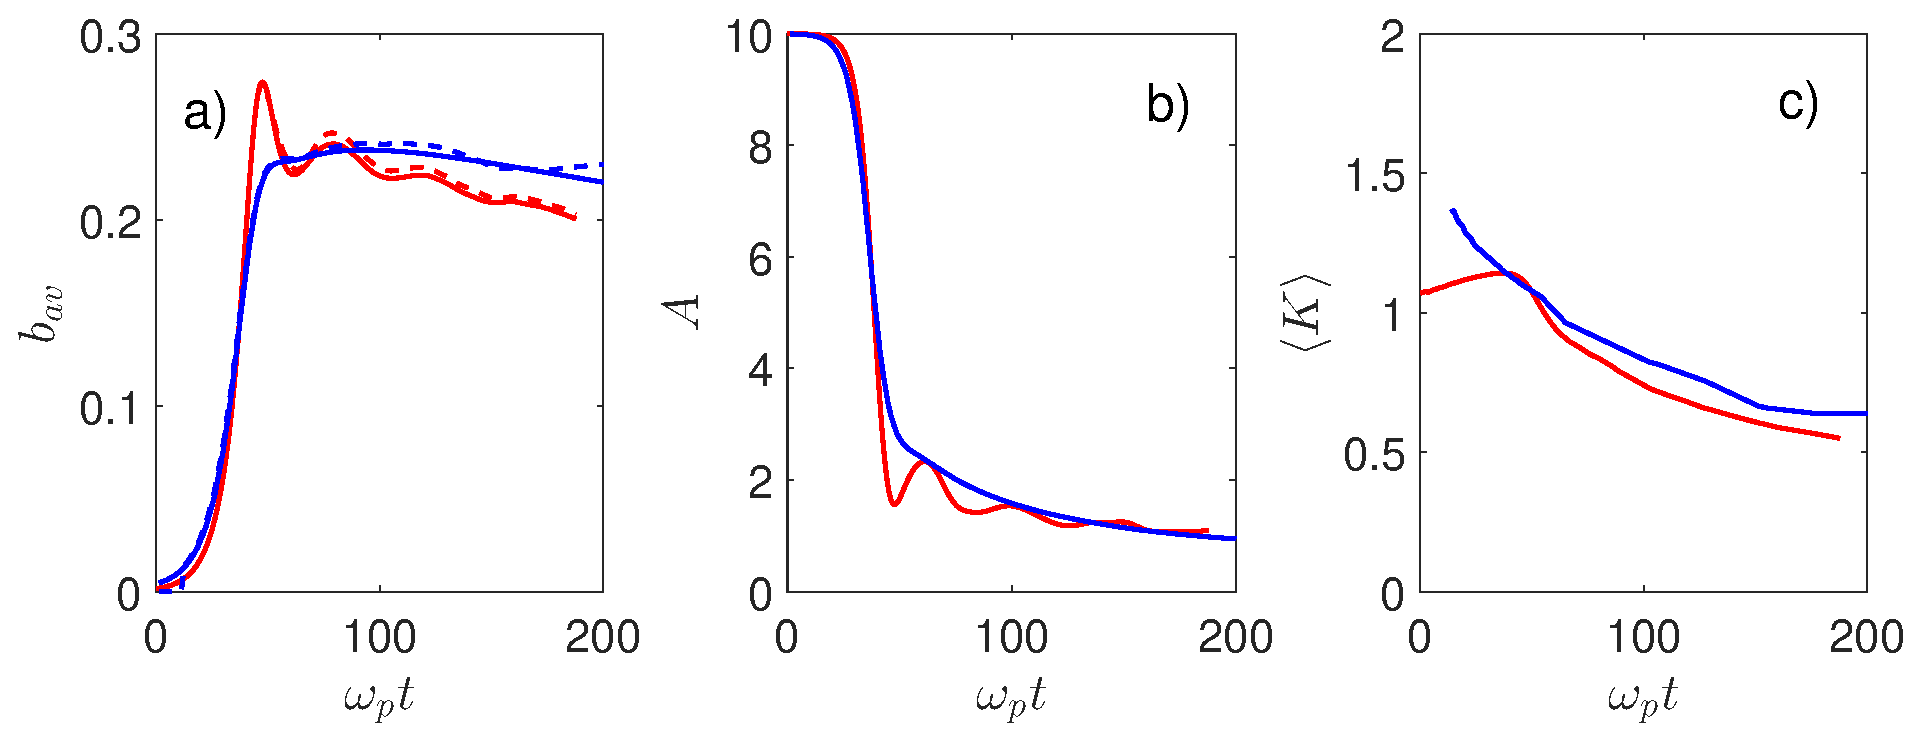
\includegraphics[width=1\linewidth]{part2/fig16.eps}
\caption{Эволюция (a) среднеквадратичного магнитного поля $b_{av}$ (сплошная линия) и оценки этой величины~(\ref{eq:otsenka2d})~(штрихи), а также (b) параметра анизотропии $A$ и (c) характерного волнового числа $\langle K\rangle$ согласно численному квазилинейному моделированию (красный цвет) и расчетам методом частиц в ячейках (синий цвет) в аксиально симметричной задаче при $A_0=10$.}
\label{fig:evol2d}
\end{figure}
Остановимся теперь на ситуации с высокой начальной анизотропией, $A_0=10$, опять опираясь на во многом идентичные результаты расчетов с использованием квазилинейного подхода и метода частиц в ячейках. Как показывает сравнение рис. \ref{fig:sravnenie_FR2dax_3im} и \ref{fig:sravnenie_FR1d_A10}, не только качественное, но и количественное отличие деформаций функции распределения электронов по скоростям в одномерной и двумерной задачах не очень велико. Впрочем, в последней линии уровня этой функции являются более овальными, менее прямоугольными, что соответствует более сглаженной, менее анизотропной форме, хотя все равно значительно отличной от бимаксвелловской во всей области скоростей порядка тепловых. При этом падение параметра анизотропии $A$ в процессе насыщения неустойчивости происходит немного плавнее, но и немного глубже, так что насыщающее магнитное поле $b_{av}$ тоже оказывается немного выше и после резкого нарастания очень медленно затухает, слегка осциллируя в противофазе с анизотропией на величину порядка нескольких процентов; ср. рис. \ref{fig:evol1d_QL_A10} и \ref{fig:evol2d}. 

Согласно рис. \ref{fig:dinspectrA10_1d} и \ref{fig:dinspectrA10_2d}, эволюция одномерного и двумерного спектра вейбелевской турбулентности в целом однотипна, а волновое число, отвечающее его максимуму (и почти совпадающее со средним значением $\langle K\rangle$), смещается в длинноволновую сторону примерно по одному и тому же степенному закону $t^{-1/2}$ (см. также рис. \ref{fig:evol2d}c; этот закон отмечался нами ранее~\cite{Borodachev2016_Radiofiz,Nechaev2019_Radiophys}). Важным, однако, представляется выявление следующих отличий в спектре двумерной турбулентности, вычисленном в квазилинейном подходе и с помощью кода EPOCH при высокой начальной анизотропии $A_0=10$. Именно, с началом стадии насыщения, $\wpl t > 60$, в коротковолновой части спектра, $K > K_\mathrm{opt}$, квазилинейный расчет демонстрирует осцилляторное поведение мод, тогда как оно отсутствует в аналогичном расчете методом частиц в ячейках, демонстрирующем резкое и существенное, по меньшей мере двукратное, расширение спектра в коротковолновую сторону. Этих отличий не было при низкой начальной анизотропии $A_0=0.25$, а также в одномерной турбулентности ни при какой начальной анизотропии. Указанное расширение спектра особенно наглядно видно на рис. \ref{fig:dinspectrA10_2d}b на больших временах $\wpl t =$ 160 и 280, когда квазилинейный расчет (сплошные кривые) показывает сильное смещение крутого правого крыла спектра в длинноволновую сторону, а более точный расчет кодом EPOCH (штрихи) сохраняет правое крыло гораздо более коротковолновым и пологим. Отметим, кстати, что соответствующие степенные показатели -3.5 и 3 правого и левого крыльев спектра двумерной турбулентности сильно отличаются от аналогичных показателей -10 и 2 спектра одномерной турбулентности при той же величине $A_0=10$, что отчасти связано с разным уровнем заданных начальных амплитуд мод. 



\begin{figure}[t]
\centering
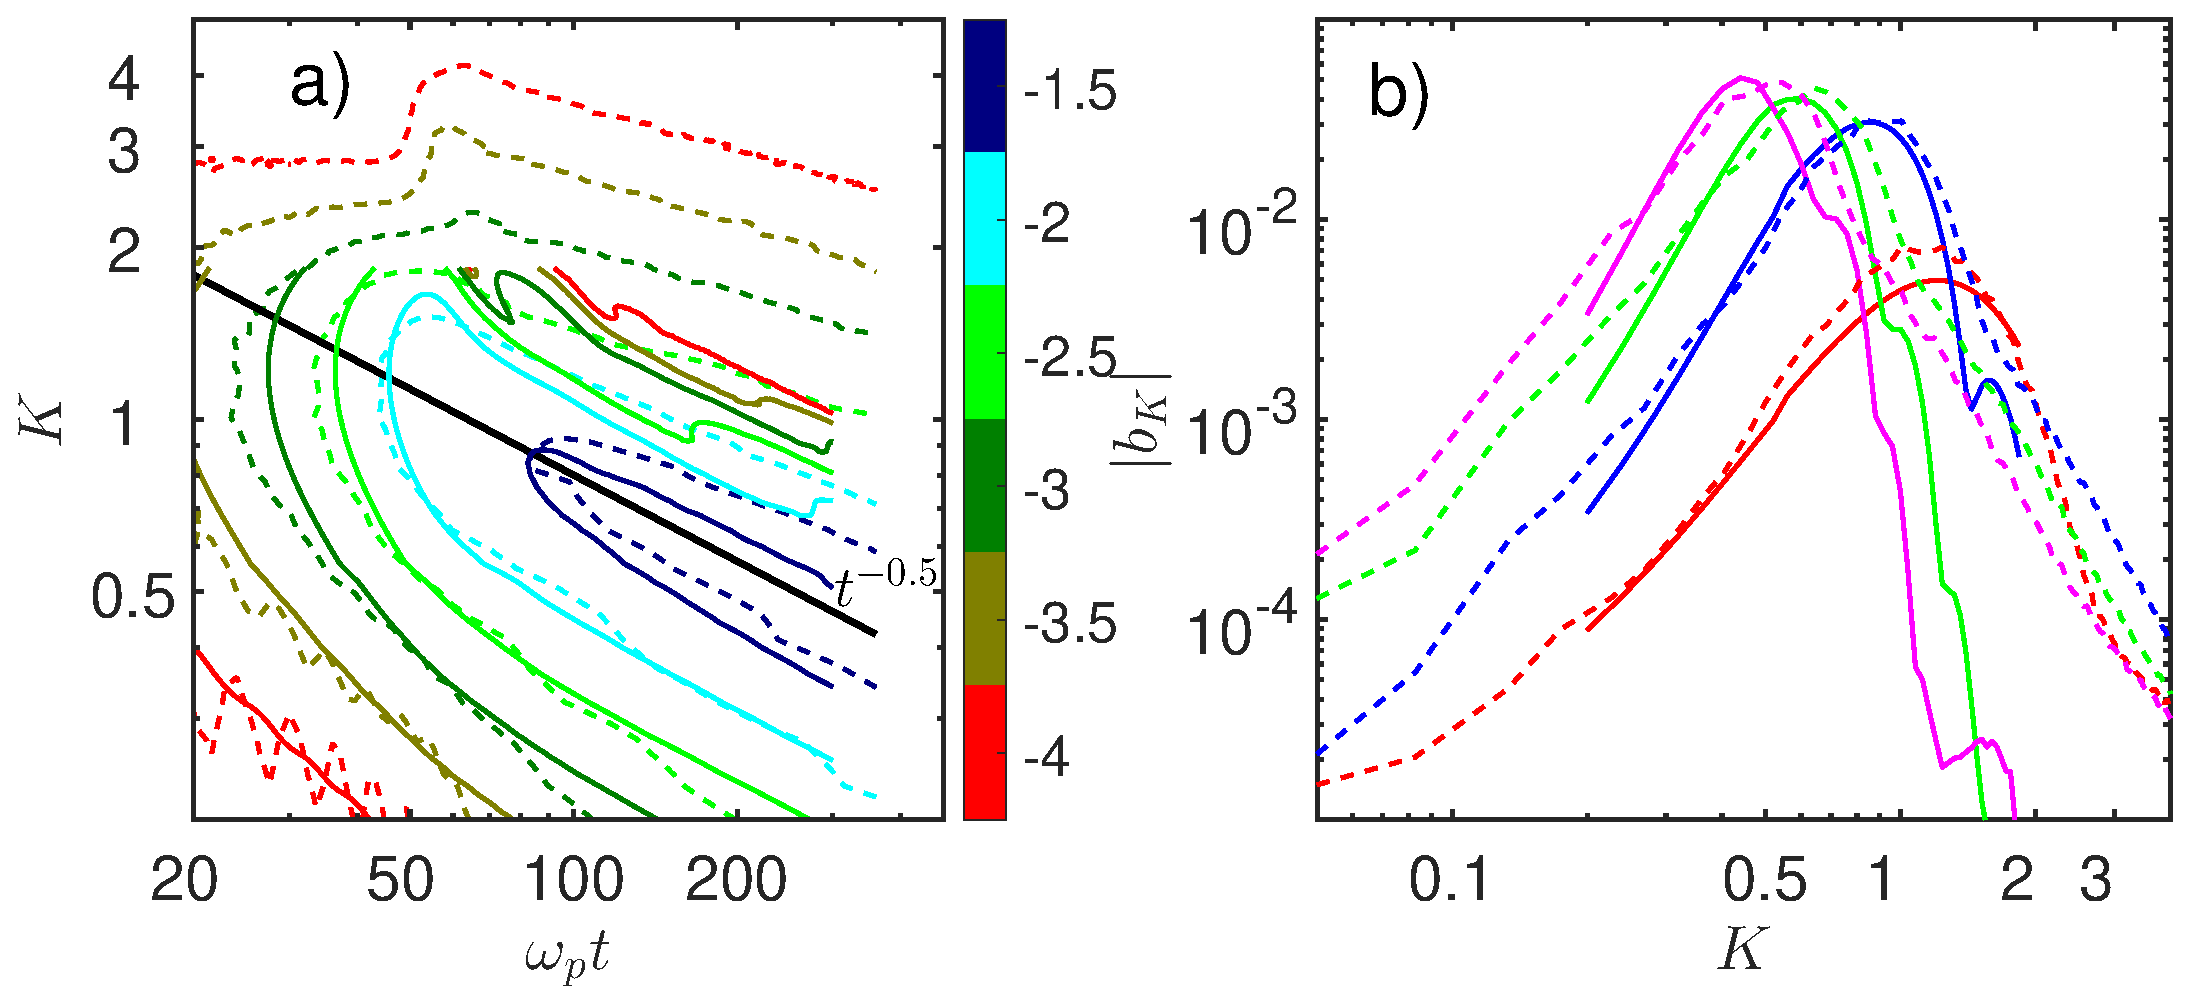
\includegraphics[width=0.9\linewidth]{part2/fig17.eps}
\caption{Эволюция спектра турбулентности, найденная в аксиально симметричных расчетах методом частиц в ячейках (штрихи) и в рамках квазилинейного подхода (сплошная линия), в двойном логарифмическом масштабе: (a)~линии уровня логарифма амплитуд мод магнитного поля $|b_K|$; 
(b)~спектр $|b_K|$ магнитного поля в моменты времени $\wpl t$, равные 40 (красный цвет), 80 (синий), 160 (зеленый) и 280 (розовый). Начальная анизотропия $A_0=10$.
}
\label{fig:dinspectrA10_2d}
\end{figure}
Причина установленных отличий, скорее всего, заключается в четырехволновом взаимодействии мод, не учитывающимся в квазилинейной системе уравнений (\ref{eq:f0.4})-(\ref{eq:oper.4}). Последняя благодаря этому обстоятельству позволяет выявить в моделировании методом частиц в ячейках нелинейные эффекты, отличные от квазилинейных. Сравнение расчетов одной и той же задачи в рамках этих двух подходов полезно провести путем анализа динамики отдельных мод двумерной вейбелевской турбулентности с использованием рис.~\ref{fig:evol_garm}. Расчет кодом EPOCH (штрихи) показывает, что с наступлением насыщения турбулентности достаточно коротковолновые моды, вопреки квазилинейному приближению (сплошные линии), не следуют осцилляторной динамике и экспоненциальному затуханию с легко вычисляемыми показателями порядка 0.01 - 0.1 (что примерно вдвое больше, чем для аналогичной одномерной турбулентности; ср. рис.~\ref{fig:evol_garmA010_1d}). Напротив, эти моды лишь частично, в небольшой мере отслеживают первую <<квазилинейную>> осцилляцию и довольно быстро переходят к медленному примерно степенному затуханию с показателями в небольшом интервале значений от -1 до -1.3, по-видимому, испытывая эффективную подкачку за счет четырехволнового взаимодействия немного более длинноволновых мод, имеющих достаточно большие амплитуды и расположенных в центральной части текущего спектра. 

\begin{figure}[b]
\centering
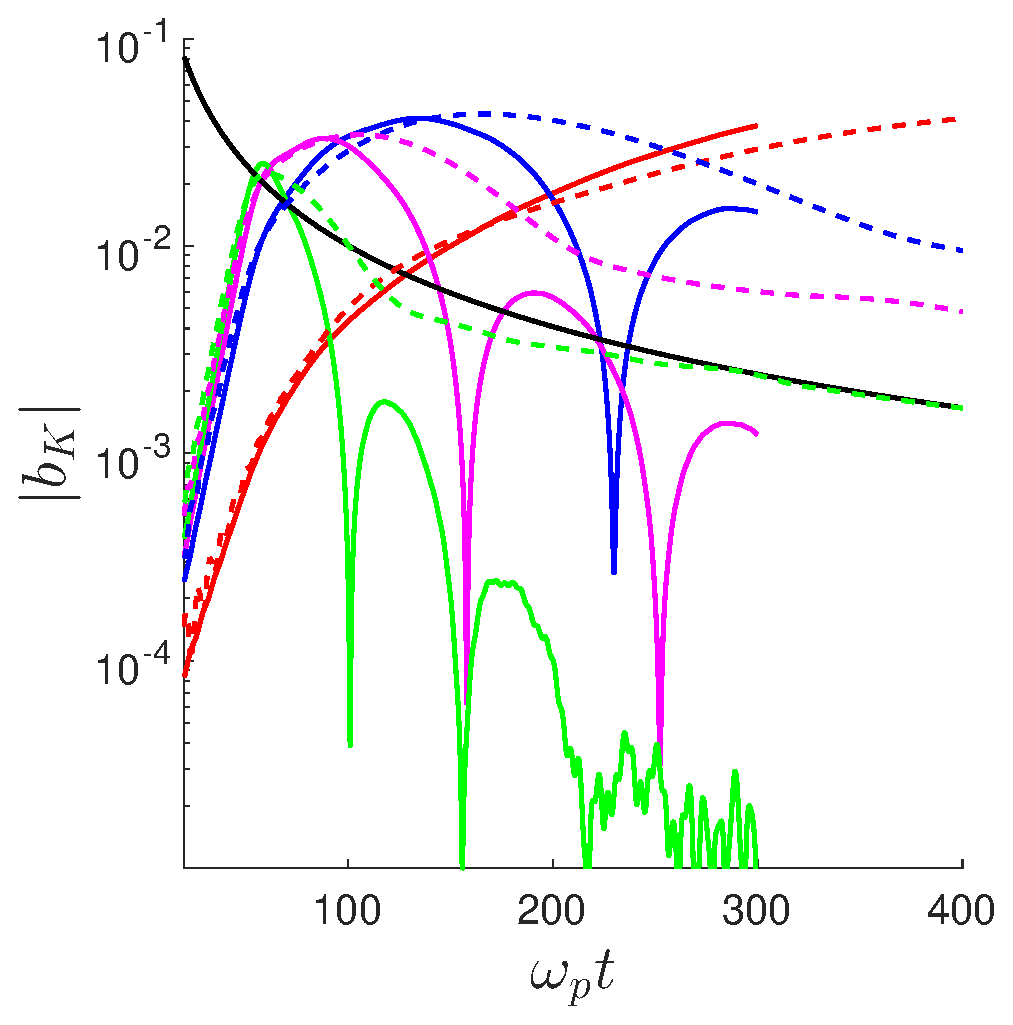
\includegraphics[width=0.5\linewidth]{part2/fig18.eps}
\caption{Эволюция четырех типичных мод ($K=0.36$ --- красный цвет, $K=0.68$ --- синий, $K=0.88$ --- розовый, $K=1.2$ --- зелёный), взятых из спектра рис. \ref{fig:dinspectrA10_2d}. Оптимальное волновое число $K_\mathrm{opt}\approx1.2$. Черная линия соответствует степенной зависимости $t^{-4/3}$.}
\label{fig:evol_garm}
\end{figure}
Вместе с тем, значительно более длинноволновые моды находятся, вплоть до своего насыщения, на промежуточной стадии приблизительно степенного роста с показателями порядка 1 - 2 (что в два-три раза меньше, чем для аналогичной одномерной турбулентности). Подобная динамика этих мод может объясняться квазилинейным образом при надлежащей зависимости от времени их инкрементов, но может быть обусловлена, хотя бы частично, все той же нелинейной подкачкой при четырехволновом взаимодействии более мощных мод из центральной части спектра турбулентности. Не исключено также, что еще более длинноволновые моды, которые только выходят или не далеко отошли от уровня шумов на стадии насыщения турбулентности, могут быть сильно, даже сверхэкспоненциально, возбуждены нелинейным образом посредством четырехволнового взаимодействия с какими-либо более мощными модами, что в результате может влиять на форму длинноволнового крыла спектра турбулентности. Данный круг вопросов требует дальнейшего детального исследования. 

Во избежание недоразумений следует отметить, что вплоть до насыщения роста среднеквадратичного магнитного поля отличия квазилинейных расчетов от расчетов методом частиц в ячейках являются весьма незначительными, даже в одномерной задаче. В итоге, квазилинейный подход позволяет корректно вычислять величину насыщающего магнитного поля вейбелевской турбулентности, что уже было продемонстрировано в конце подраздела 3.1 на рис.~\ref{fig:bsat}. Согласно ему, средний квадрат насыщающего поля двумерной турбулентности отличается от его значения для одномерной на десятки процентов при большом начальном параметре анизотропии, $A_0\gtrsim1$, и многократно при низком параметре, $A_0\lesssim1$, поскольку тогда численно найденный показатель его степенной зависимости от этого параметра оказывается близким к 2 вместо аналитически найденного показателя 5 для одномерной турбулентности (см. формулу (\ref{eq:analit_estimation})). 

Таким образом, проведенные расчеты, в том числе и для других параметров анизотропии $A_0$, показывают следующие существенные различия эволюции спектра вейбелевской турбулентности в одномерной и аксиально симметричной двумерной задачах при одинаковых начальных условиях. 

Во-первых, более богатый двумерный спектр развитых мод обеспечивает более гладкую и сильную модификацию исходной функции распределения электронов по скоростям, а следовательно, более значительные уменьшение параметра анизотропии и увеличение магнитной энергии турбулентности. При этом последующий распад образовавшихся случайных самосогласованных токовых филаментов идет эффективнее, чем для турбулентности с одномерным спектром, где квазилинейные эффекты и четырехволновое взаимодействие мод искусственно ограничены, как и свободный разлет электронов из токовых слоев.

Во-вторых, в двумерном случае автомодельный характер эволюции спектра выражен более явно, а формирование его степенных крыльев и смещение его максимума в длинноволновую сторону происходят быстрее, возможно, благодаря не только квазилинейному, но и четырехволновому взаимодействию мод. При этом зависимость соответствующих параметров спектра от начальной анизотропии плазмы выражена слабее, чем в одномерном случае, где перестройка спектра заторможена.

В-третьих, динамика отдельных мод в двумерной задаче, естественно, оказывается более сложной и многообразной, хотя в общем случае и включает в себя те же три основные стадии, что и в одномерной задаче: сначала экспоненциальное и потом примерно степенное нарастание, а после достижения максимума -  тоже спадание степенного типа. При этом в одномерной турбулентности для многих мод не все эти стадии четко выражены, но значительно заметнее квазипериодические осцилляции амплитуд мод и даже ее интегральных характеристик, вызванные, как и в двумерной турбулентности, квазилинейной модификацией анизотропии функции распределения электронов и соответствующим изменением действительных частот и инкрементов (декрементов) мод.
             % Глава 2
\chapter{Вёрстка таблиц}\label{ch:ch3}
\section{Квазилинейная систама уравнений для совместной эволюции вейбелевсой и ленгмюрвоской турбулентностей}

Для различных задач физики лабораторной и космической бесстолкновительной плазмы, включая солнечный ветер и магнитосферы звезд и планет, характерно наличие пучка энергичных заряженных частиц (электронов и/или ионов) в теплой плазме~\cite{Gary1993,Treumann1997,Marsch2006}. Даже если распределение частиц по скоростям в плазме и в пучке является изотропным максвелловским (в соответствующей  системе отсчета), для совместной системы "плазма+пучок" распределение будет анизотропным.  В результате, согласно дисперсионному анализу~\cite{Mikhailovsky1971,Fried1959,Krall1973,Tzoufras2006,Bret2010}, могут одновременно развиваться различные кинетические неустойчивости, прежде всего резонансная квазиэлектростатическая двухпотоковая неустойчивость и апериодическая квазимагнитостатическая неустойчивость вейбелевского типа, известные также как пучковая и филаментационная соответственно. 

Двухпотоковой неустойчивости подвержены продольные ленгмюровские (плазменные) волны, так что её развитие приводит к формированию коротковолновой ленгмюровской турбулентности электрического поля и плотности плазмы~\cite{Vedenov1963,Zakharov1972,VedenovRyutov1975,Krall1973,Appert1976,Yi2010,Bakunin2017,Sun2022}; при этом в общем распределении частиц образуется плато в области  скоростей между теплой плазмой и пучком.  Вследствие филаментационной неустойчивости возникает вейбелевская (магнитная) турбулентность, а именно, формируются более длинноволновые поперечные квазимагнитостатические поля и согласованные с ними токовые филаменты или слои~\cite{Weibel1959, Zhou2022,Fried1959, Kalman1968, Morse1971, Kocharovsky2016, Lazar2006, Stockem2009, SchaeferRolffs2006}; при этом уменьшается анизотропия общего распределения частиц по скоростям и его пучковая часть сглаживается.


Нас будет интересовать незамагниченная плазма, для которой двухпотоковая (пучкового типа) и филаментационная (вейбелевского типа) неустойчивости по отдельности изучены достаточно подробно, особенно в линейном приближении; см., например,~\cite{Mikhailovsky1971,Fried1959,Tzoufras2006,Hao2008,Bret2010,Moya2022}. При этом для исследования долговременной нелинейной динамики турбулентности, возникающей в результате развития изолированных двухпотоковой или филаментационной неустойчивостей, применялись как  полноценные расчеты методом частиц в ячейках~\cite{Kasaba2001,Dum1994,Yi2010,Ruyer2015,Dieckmann2009,Bret2010,Lazar2023,Nechaev2023,Kocharovsky2024,Garasev2022,Kuznetsov2025a}, так и различные приближенные подходы, прежде всего квазилинейные~\cite{Vedenov1963,VedenovRyutov1975,Appert1976,Bakunin2017,Ziebell2008,Lemons1979,Davidson1972,Ruyer2015,Kuznetsov2022,Kuznetsov2023}. 

Однако до сих пор слабо освещена проблема нелинейного взаимодействия ленгмюровской и вейбелевской турбулентности, важная для анализа таких явлений, как формирование бесстолкновительных ударных волн и структур в аккреционных дисках и колонках, взаимопроникновения соседних облаков и потоков частиц звёздного ветра, развитие корональных выбросов массы и солнечных вспышек, нагрев плазмы и изменение её кинетических свойств при инжекции пучков высокоэнергичных частиц и др.~\cite{Marcowith2016,Treumann2015,Aschwanden2005,Medvedev2006,Nishikawa2009,Kato2007,Kuznetsov2025b}. Имеющиеся выборочные работы в этом направлении исследований основаны преимущественно на расчетах методом частиц в ячейках, зачастую ограничиваются гидродинамическим режимом той или иной неустойчивости и по существу не касаются, а тем более не детализируют взаимное влияние ленгмюровской и вейбелевской  турбулентности; ср., например,~\cite{Kong2009,Ruyer2015,Bret2010,Lazar2023} (при наличии внешнего магнитного поля см. также работы~\cite{Lazar2023,Lopez2020}). Так, в обзоре~\cite{Bret2010}, являющемся, по-видимому, наиболее полным для интересующей нас задачи в отсутствие внешнего магнитного поля, обсуждаются условия насыщения и возможные нелинейные локализованные структуры в турбулентности каждого типа, но не изучается влияние изменения функции распределения частиц под действием турбулентности одного типа на развитие другой, хотя и упоминается возможность их последовательного развития.

В настоящей работе предпринято детальное изучение одного из механизмов взаимного влияния указанных неустойчивостей для кинетического режима их нарастания, насыщения и последующей релаксации сформировавшейся слабой турбулентности. А именно, проанализировано, как каждое из турбулентных полей - в основном электрическое или магнитное для двухпотоковой или филаментационной неустойчивостей соответственно - изменяет общую среднюю по пространству функцию распределения частиц по скоростям и тем самым модифицирует ход сопутствующей неустойчивости. В подобном квазилинейном подходе~\cite{VedenovRyutov1975,Appert1976,Kuznetsov2022,Kuznetsov2023} каждая мода турбулентности эволюционирует локально во времени согласно её инкременту (декременту), вычисляемому в линейном приближении с использованием указанной мгновенной функции распределения частиц. При этом рассматриваются условия, в которых, как подтверждают тестовые расчеты методом частиц в ячейках, исключена определяющая роль других возможных механизмов нелинейного изменения спектра обеих типов турбулентности, например, появление множественных ленгмюровских солитонов с нескомпенсированным зарядом или z-пинчей тока и систематическое трех- или четырехволновое взаимодействие отдельных мод (пространственных гармоник).

С этой целью построена замкнутая квазилинейная система уравнений, разработан оригинальный численный код её решения и с его помощью рассчитана одновременная нелинейная динамика большого числа (многих тысяч) ленгмюровских и вейбелевских мод турбулентной плазмы в кинетическом приближении, когда допустимые инкременты $\gamma$ и соответствующие волновые числа $k$ всех мод удовлетворяют неравенству $\gamma\ll kv_T$, где $v_T$~--- тепловая скорость. В результате установлена роль квазилинейного взаимодействия мод в эволюции спектров ленгмюровской и вейбелевской турбулентности, а также найдена динамика среднеквадратичных электрического и магнитного полей в ней и указан неравномерный характер уменьшения анизотропии распределения частиц по скоростям и увеличения тепловой энергии плазмы (нагрев) в поперечном к пучку направлении. 

Такой подход соответствует классическому квазилинейному описанию ленгмюровской турбулентности~\cite{VedenovRyutov1975,Appert1976} и развитому в работах~\cite{Kuznetsov2022,Kuznetsov2023} описанию турбулентности вейбелевского типа. Преимуществами подобного подхода перед моделированием методом частиц в ячейках являются возможность свободно выбирать диапазон представляющих интерес волновых векторов мод и регулировать начальный уровень их амплитуд. Это позволяет не только по отдельности верифицировать квазилинейное описание филаментационных и двухпотоковых мод путем сравнения получающихся частных результатов с найденными ранее результатами расчетов методом частиц в ячейках, но и сравнить независимую динамику спектра тех и других мод с их совместной динамикой. Немаловажной является и меньшая требовательность квазилинейных расчетов к вычислительным ресурсам, загруженность которых в расчетах методом частиц в ячейках оказывается многократно выше, в частности, из-за необходимости использования большого числа частиц  для корректного описания резонансных эффектов кинетической двухпотоковой неустойчивости~\cite{Lotov2015}.  

Для простоты представленные результаты ограничены решением начальной двумерной задачи для однородной незамагниченной нерелятивистской системы "плазма+пучок", в которой фоновая плазма и пучок включают холодные ионы и имеют одинаковую тепловую скорость $v_T$ (и температуру $T$) электронов, а направленная вдоль оси $y$ скорость пучка $v_s$ не сильно превышает тепловую скорость. В рассматриваемых условиях эффекты появления локализованного пространственного заряда и z-пинчевания токов плазмы отсутствуют~\cite{Tzoufras2006,Hao2008,Kocharovsky2024,Garasev2022}. Исследуется квазилинейная эволюция спектра  двухпотоковых (ленгмюровских) мод, т.е. фактически электростатических возмущений с волновыми векторами, в основном сонаправленными с пучком, и спектра филаментационных (вейбелевских) мод, т.е. поперечных электромагнитных возмущений с почти ортогональными пучку волновыми векторами~\cite{Bret2004,Bret2010}. Эти два спектра мод хорошо разделены по направлению и величинам волновых векторов и для их описания используются две прямоугольные сетки волновых векторов, плотно покрывающие область неустойчивости~(рис. \ref{fig:1}).  
\begin{figure}[h]

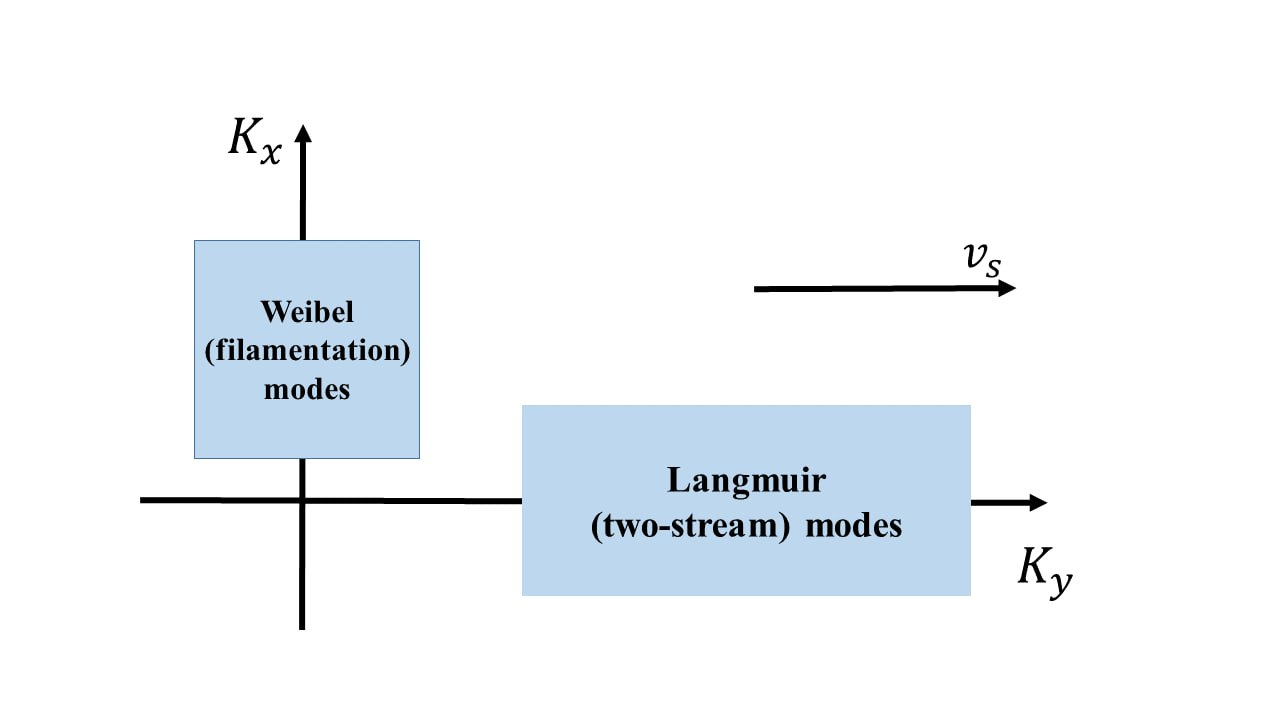
\includegraphics[width=1\linewidth]{part3/1.jpg}
\captionstyle{normal}
\caption{Схема расчетной плоскости, включающая две прямоугольные сетки волновых векторов для генерируемых спектров филаментационных и двухпотоковых мод.}
\label{fig:1}
\end{figure}

Квазилинейная система уравнений, используемая для моделирования, представлена в разделе 2. В разделах 3 и 4 обсуждаются результаты численных расчетов для двух характерных наборов параметров плазмы и пучка, отвечающих качественно различной динамике спектров мод. В заключении подводятся итоги и обсуждаются возможные направления дальнейших исследований.



Для бесстолкновительной плазмы, в которой на рассматриваемых временах порядка десяти времен насыщения неустойчивости можно пренебречь движением тяжелых ионов, самосогласованные уравнения Власова~-- Максвелла для функции распределения электронов $f(v_x , v_y , x, y, t)$, включающей их концентрацию $N (x, y, t)$, и электрического $\vec{E}=(E_x, E_y, 0)$ и магнитного $\vec{B}=(0, 0, B_z)$ полей имеют вид~\cite{Mikhailovsky1971,Krall1973,Baumjohann2012,Vedenov1963,VedenovRyutov1975,Bakunin2017,Kocharovsky2016}:
\begin{eqnarray}
    \dfrac{\partial f}{\partial t}+\vec{v}\dfrac{\partial f}{\partial \vec{r}}+\dfrac{e}{\me} \left(\vec{E}+\dfrac{1}{c}\left[\vec{v},\vec{B}\right]\right) \dfrac{\partial f}{\partial \vec{v}}=0, \\
    %
    \label{eq:maxw1} 
    \nabla \times \vec{B}=\dfrac{1}{c}\dfrac{\partial \vec{E}}{\partial t}+\dfrac{4\pi}{c}\vec{j}, \\
    %
    \label{eq:maxw2}
    \nabla \times \vec{E}=-\dfrac{1}{c}\dfrac{\partial \vec{B}}{\partial t},
\end{eqnarray}
где $c$~--- скорость света в вакууме, $e$ и $\me$~--- заряд и масса электрона, $\vec{j}=e\iint^{+\infty}_{-\infty}\vec{v}f(v_x , v_y , x, y, t) dv_x dv_y$~--- плотность тока, $N=\iint^{+\infty}_{-\infty}f(v_x , v_y , x, y, t)dv_xdv_y$ и учтено, что векторы координаты и скорости имеют только две компоненты, $\vec{r}=(x , y ,0)$ и $\vec{v}=(v_x , v_y ,0)$, согласно двумерной постановке задачи. 

При прохождении через фоновую плазму достаточно широкого пучка частиц, поперечный размер которого много больше плазменного скин-слоя, возникает обратный ток, так что $n_b\beta_{b}=n_s\beta_{s}$~\cite{Shukla2018,Jia2013,Karlick2008}, где $n_i$ и $\beta_i=v_i/c$~--- начальная концентрация и безразмерная направленная скорость фракций частиц: индексы $b$ и $s$ соответствуют фону и пучку. Поэтому используемое в работе обезразмеренное начальное распределение электронов по скоростям имеет вид
\begin{equation}
\label{eq:bp}
    \Psi_0(\vec{\beta})=\dfrac{n_b}{\pi\beta_T^2} \exp\left(-\dfrac{\beta_x^2}{\beta_T^2}-\dfrac{\left(\beta_y+\beta_{b}\right)^2}{\beta_T^2}\right)+\dfrac{n_s}{\pi\beta_T^2 } \exp\left(-\dfrac{\beta_x^2}{\beta_T^2}-\dfrac{\left(\beta_y-\beta_{s}\right)^2}{\beta_T^2}\right).  
\end{equation}
Выше $\beta_{x,y}={v_{x,y}}/{c}$, т.\,е. $\vec{\beta}=\vec{v}/{c}$, $\beta_T=\sqrt{2nk_bT/m_e}/c$, где включена постоянная Больцмана $k_b$. 

Квазилинейный подход к описанию взаимного влияния ленгмюровской и вейбелевской турбулентностей основан на разложении по пространственным модам решения уравнений  Максвелла~-- Власова~\cite{Baumjohann2012} с шумоподобным примерно равномерным по спектру начальным возмущением электромагнитного поля для мод филаментационной и двухпотоковой неустойчивостей. Такое разложение особенно эффективно тогда, когда ключевую роль играет интегральное нелинейное взаимодействие мод посредством их совместного изменения средней по пространству функции распределения частиц по скоростям. Последняя определяет текущие значения инкрементов (декрементов) и действительных частот всех рассматриваемых мод, в остальном эволюционирующих независимо. 
Подобное квазилинейное описание турбулентности оправдано в условиях случайности фаз мод и отсутствия захвата частиц электрическими или магнитными полями отдельных гармоник либо локализованных в пространстве структур, что обычно справедливо в кинетическом режиме развития неустойчивости и дальнейшей нелинейной динамики слабой турбулентности~\cite{GaleevSagdeev1969,Bakunin2017,Kuznetsov2023}. Наличие большого числа однотипных не сфазированных мод, достаточно плотно заполняющих значимую область волновых векторов, гарантирует гладкость формы и плавность изменения функции распределения частиц по скоростям, исключая артефакты когерентной интерференции и отрицательные значения этой функции всюду, кроме, возможно, несущественной, содержащей крайне мало частиц, области их скоростей, очень больших по сравнению с тепловыми скоростями. При этом по существу реализуется адиабатическая динамика каждой моды, непрерывно подстраивающейся к изменяющейся функции распределения электронов. 

В рассматриваемом двумерно-неоднородном случае для описания вейбелевской турбулентности используется сетка из часто расположенных и перекрывающих всю турбулентную область волновых векторов $m_W \cdot s_W$ неколлинеарных мод с хаотическими фазами и примерно одинаковыми исходными амплитудами при $t=0$. Аналогичная сетка $m_L \cdot s_L$ неколлиннеарных мод выбрана и для описания ленгмюровской турбулентности~(рис. \ref{fig:1}), где $m_i$ и $s_i$~--- количество заданных дискретных значений соответствующих ортогональных проекций $\vec{K}\vec{x_0}$ и $\vec{K}\vec{y_0}$ волновых векторов. В этом представлении магнитное поле имеет вид суммы по целочисленному векторному индексу $\vec{n}=(n_x,n_y)$:
\begin{equation}
    B_z(t,x,y)= \mathrm{Re} \Biggr[ \sum^{m_W,s_W}_{n_x,n_y=1}B_{k_\vec{n}}(t)\exp(- ik_{n_{x}}x - ik_{n_{y}}y)\Biggr]+ \mathrm{Re} \Biggr[\sum^{m_L,s_L}_{n_x,n_y=1}B_{k_\vec{n}}(t)\exp(- ik_{n_{x}}x - ik_{n_{y}}y)\Biggr].
\end{equation}
Аналогичный вид имеют обе компоненты электрического поля $E_x$ и $Ey$, а также возмущение 
функции распределения $\delta f(t,x,y)$. Получаемая из уравнений Власова-Максвелла квазилинейная система  $4(m_W\cdot s_W+m_L\cdot s_L)+1$ уравнений для усредненной в пространстве компоненты функции распределения электронов по скоростям $\psi_0$,  а также безразмерных комплексных амплитуд её возмущений $\psi_{K_{\vec{n}}}$ и возмущений магнитного $b_{K_{\vec{n}}}$ и двух компонент электрического  $e_{x{K_{\vec{n}}}}$ и $e_{y{K_{\vec{n}}}}$ полей имеет следующий вид:
~\ref{} 
\begin{equation}
\label{eq14}
    \dfrac{\partial \psi_0}{\partial \tau} 
    + \mathrm{Re}\Biggr[\sum\limits^{m_W,s_W}_{n_x,n_y=1} \hat \Phi(b_{K_{\vec{n}}},\overrightarrow{e}_{K_{\vec{n}}},\psi_{K_{\vec{n}}}^*) 
     \Biggr]+ \mathrm{Re}\Biggr[\sum\limits^{m_L,s_L}_{n_x,n_y=1} \hat \Phi(b_{K_{\vec{n}}},\overrightarrow{e}_{K_{\vec{n}}},\psi_{K_{\vec{n}}}^*) 
     \Biggr]=0,
\end{equation}
\begin{equation}
    \label{eq15}
    \dfrac{\partial \psi_{K_{\vec{n}}}}{\partial \tau}+iK_{n_x}\beta_x\psi_{K_{\vec{n}}}+iK_{n_y}\beta_y\psi_{K_{\vec{n}}}+2\hat \Phi(b_{K_{\vec{n}}},\psi_0)=0,
\end{equation}
\begin{equation}
    \dfrac{\partial b_{K_{\vec{n}}}}{\partial \tau}=-ie_{y{K_{\vec{n}}}}K_{n_x}+ie_{x{K_{\vec{n}}}}K_{n_y},
\end{equation}
\begin{equation}
    \dfrac{\partial e_{x{K_{\vec{n}}}}}{\partial \tau}=ib_{K_{\vec{n}}}K_{n_y}-\beta_{\|}^{-1}\iint\limits^{+\infty}_{-\infty}\beta_x\psi_{K_{\vec{n}}}(\tau,\beta_x,\beta_y)d\beta_xd\beta_y,
\end{equation}
\begin{equation}
\label{eq19}
    \dfrac{\partial e_{y{K_{\vec{n}}}}}{\partial \tau}=-ib_{K_{\vec{n}}}K_{n_x}+\beta_{\|}^{-1}{\iint\limits^{+\infty}_{-\infty}\beta_y\psi_{K_{\vec{n}}}(\tau,\beta_x,\beta_y)d\beta_xd\beta_y} .
\end{equation}
Здесь использованы безразмерные время, волновое число, а также нормированные (комплексные) гармоники магнитного поля и функции распределения электронов по скоростям: 
\begin{equation}
    \label{eq19plus1}
    \tau=\wpl t, \
    K=\dfrac{kc}{\wpl}; \ 
    \wpl^2=\dfrac{4\pi Ne^2}{\me},\
    b_{K_{\vec{n}}}=\dfrac{B_{K_{\vec{n}}}}{\sqrt{8\pi N T}},\
    T=\dfrac{m_ec^2\beta_{T}^2}{2};\
    \psi_{K_{\vec{n}}}=\dfrac{c^2f_{ K_{\vec{n}}}}{N}.\ 
\end{equation}

Комплексные компоненты электрического поля $e_{x{K_{\vec{n}}}}$ и $e_{y{K_{\vec{n}}}}$ нормированы так же, как магнитное поле $b_{K_{\vec{n}}}$. В уравнениях (\ref{eq14})-(\ref{eq15}) для сокращения записи введен оператор
\begin{equation}
\label{eq:operator}
    \hat \Phi(b_{K_n},e_{x{K_{\vec{n}}}},e_{y{K_{\vec{n}}}},\psi(\vec{\beta}))=\dfrac{e_{y{K_{\vec{n}}}}}{2}\dfrac{\partial \psi(\vec{\beta})}{\partial \beta_y}+\dfrac{e_{x{K_{\vec{n}}}}}{2}\dfrac{\partial \psi(\vec{\beta})}{\partial \beta_x}-\dfrac{b_{K_n}}{2} \left(\beta_x\dfrac{\partial \psi(\vec{\beta})}{\partial \beta_y}-\beta_y\dfrac{\partial \psi(\vec{\beta})}{\partial \beta_x}\right).
\end{equation}

Представленная система интегро-дифференциальных уравнений (\ref{eq14})--(\ref{eq19}) с оператором (\ref{eq:operator}) решалась численно стандартным методом Стёрмера~-- Верле (Leapfrog)~\cite{Birdsall2018}. Параметр анизотропии $A$, равный отличию от единицы отношения полной энергии электронов в продольном $W_\|$ и поперечном $W_\perp$ к скорости пучка направлении, является ключевым для квазилинейного описания вейбелевской турбулентности~\cite{Weibel1959,Davidson1972,Lemons1979,Tzoufras2006,Kuznetsov2023}. Начальное значение параметра анизотропии $A_0$ для распределения электронов вида~(\ref{eq:bp}), определяется исходным отношением энергий их направленного и теплового движений:
%~(\ref{anisotropy}):

\begin{equation}
A=\frac{W_\|}{W_\perp}-1;~~~A(\tau=0)=A_0=\frac{n_s\beta_s^2+n_b\beta_b^2}{(n_s+n_b)\beta_T^2/2}.
\label{anisotropy}
\end{equation}

Шаг по времени $d\tau$ и шаг сетки, аппроксимирующей распределение электронов в пространстве скоростей, $d\beta$, выбирались хотя бы на порядок уступающими минимальному масштабу по времени и по скорости соответственно. Количество как филаментационных, так и ленгмюровских пространственных мод  $m_W\cdot s_W+m_L\cdot s_L$ в типичных расчетах составляло несколько тысяч  и выбиралось из условия как независимости (с точностью до нескольких процентов) вычисляемых среднеквадратичного магнитного и электрического поля от дальнейшего увеличения числа мод, так и условия перекрытия резонансов~\cite{GaleevSagdeev1969,Bakunin2017} для энергонесущих ленгмюровских мод на протяжении всего изучаемого отрезка нелинейной эволюции. Для всех расчетов проверялась справедливость кинетического приближения, т.е. условие малой величины инкремента $\gamma\ll K\beta_T$, причем для определенности начальная тепловая скорость электронов полагалась равной $\beta_{T}=0.1$. 

\section{Квазилинейный механизм подавления ленгмюровской турбулентности филаментационными модами}

Несмотря на то что двухпотоковая неустойчивость вызвана относительно небольшим числом резонансных электронов, так как экспоненциальный рост квазиэлектростатических полей обусловлен наличием ограниченного участка немонотонности распределения электронов по скоростям, её инкремент для нерелятивистских пучков с направленной скоростью $\beta_s$ существенно выше тепловой скорости $\beta_{T}$, как правило, значительно превосходит филаментационный~\cite{Bret2010}. Нарастание амплитуды ленгмюровских волн в ходе двухпотоковой неустойчивости происходит до тех пор, пока указанная немонотонность не сгладится и не сформируется так называемое квазилинейное плато.  В результате часть энергии направленного движения электронов распределяется между генерируемыми полями и тепловой энергией электронов, так что их распределение в пространстве скоростей частично изотропизуется~\cite{GaleevSagdeev1969}. В одномерном приближении на этом квазилинейная динамика ленгмюровской турбулентности фактически останавливается. Однако в рассматриваемом двумерном случае плато продолжает деформироваться за счет затухания Ландау, прежде всего, не коллинеарных с пучком наклонных мод, так что спектр квазиэлектростатической турбулентности постепенно становится всё более коротковолновым, а следы пучка в пространстве скоростей размываются~\cite{Appert1976,Yi2010}. Таким образом, без учета магнитной турбулентности в системе "плазма+пучок" происходит очень медленная, квазилинейная изотропизация распределения частиц и затухание электрического поля. 

В отсутствие эффектов пространственного заряда, гарантированном принятым условием одинаковой температуры фона и пучка, филаментационной неустойчивости подвержено любое анизотропное распределение электронов вида~(\ref{eq:bp})~\cite{Tzoufras2006}. Поэтому в типичных бесстолкновительных условиях филаментационная неустойчивость системы "плазма+пучок" неизбежна и продолжается даже после насыщения двухпотоковой. Тем не менее, вызванное ленгмюровской турбулентностью уменьшение параметра анизотропии распределения электронов ослабляет инкремент филаментационных мод и снижает уровень насыщения их роста. В свою очередь, развившаяся магнитная турбулентность, порождаемая филаментационными модами, как будет ясно из дальнейшего, может деформировать распределение электронов по скоростям в резонансной с ленгмюровскими волнами области, а следовательно, способна значительно повлиять на затухание Ландау последних.

Для демонстрации сказанного обратимся к результатам квазилинейного расчета эволюции системы с начальными  параметрами $n_s=0.055n_b$ и $\beta_s=2.5\beta_T$, для которых согласно линейной теории~\cite{Mikhailovsky1971,Davidson1972} наибольшим инкрементом $\gamma_L\approx0.017\omega_p$ обладает ленгмюровская продольная мода с волновым числом $K_y\approx4.2$, а среди филаментационных наиболее неустойчива поперечная мода с волновым числом $K_x\approx0.44$ и инкрементом $\gamma_F\approx9*10^{-3}\omega_p$, примерно вдвое меньшим ленгмюровского. Для этих параметров начального распределения частиц сравнение поправок к нему для расчета, учитывающего исключительно двухпотоковые моды, и для расчета, описывающего совместную динамику ленгмюровской и вейбелевской турбулентности, показывает, что влияние филаментационных мод на распределение электронов намного значительнее, чем ленгмюровских, и что деформация распределения под этим влиянием происходит в том числе и в резонансной области для коллинеарных с пучком ленгмюровских мод, являющихся основными энергонесущими модами в данный момент времени  (рис.\ref{fig:FR1}). Указанные на данном рисунке границы резонансной области $\beta_{y,min}=1/K_{y,max}$ и $\beta_{y,max}=1/K_{y,min}$ примерно оценены из условия черенковского резонанса, в котором для простоты частота ленгмюровских волн считается равной плазменной, а поперечная компонента волнового числа полагается равной нулю: $K_x=0$. 

\begin{figure}[h]
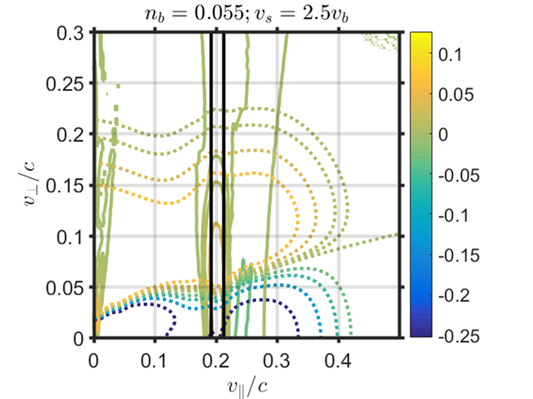
\includegraphics[width=0.5\linewidth]{part3/FR1.png}
\centering
\captionstyle{normal}
\caption{Вычисленные для момента времени $\omega_pt=5000$ линии уровня нормированной на максимум начального распределения поправки к пространственно однородной компоненте функции распределения электронов по скоростям (\ref{eq:bp}), которая в начальный момент времени являлась максвелловской с пучком, в случае учета только двухпотоковых мод (сплошная) и в случае совместной эволюции ленгмюровской и вейбелевской турбулентности (пунктир). Параметры начального распределения (4): $n_s=0.055n_b$, $\beta_s=2.5\beta_T$, $\beta_T=0.1$. Вертикальные черные линии выделяют область скоростей электронов, резонансно взаимодействующих с коллинеарными пучку ленгмюровскими модами, являющимися основными энергонесущими в данный момент времени.}
\label{fig:FR1}
\end{figure}

В отсутствие филаментационных мод на интервалах времени, не более чем в 6 раз превышающих время насыщения двухпотоковой неустойчивости, среднеквадратичное электрическое поле ленгмюровских мод находится на примерно постоянном уровне. Включение филаментационных мод приводит к тому, что сразу после окончания экспоненциального роста этих мод с наибольшим инкрементом, означающего начало существенной анизотропной деформации общей функции распределения электронов по скоростям и переход к нелинейной стадии магнитной турбулентности, начинается довольно резкое затухание ленгмюровских волн~(рис.\ref{fig:average1}a). Декремент затухания каждой ленгмюровской моды определяется формой распределения электронов по скоростям только в резонансной для этой моды области. Поскольку с течением времени спектр ленгмюровских волн смещается в коротковолновую область~(рис.\ref{fig:average1}d), то скорость затухания среднеквадратичного электрического поля ленгмюровских мод зависит от промежутка времени между насыщением роста двухпотоковой и филаментационной неустойчивостей, а значит, от амплитуд начальных возмущений электрического и магнитного полей~(иллюстрация дана на рис.\ref{fig:average1}a). При этом среднеквадратичное индукционное электрическое поле филаментационных мод мало в сравнении с полем ленгмюровских мод на протяжении всей эволюции. Аналогично, малым является и среднеквадратичное магнитное поле ленгмюровских мод в сравнении с полем филаментационных.

Как уже сказано выше, вследствие квазилинейного взаимодействия между ленгмюровскими волнами характерное продольное волновое число их спектра $\langle K_\|\rangle$ увеличивается ~(рис.\ref{fig:average1}d). В приводимом примере это увеличение останавливается на уровне около 20\% примерно на временах, на порядок превышающих время насыщения ленгмюровской турбулентности, и почти не зависит от вейбелевской турбулентности. Однако благодаря её влиянию, а именно, квазилинейной деформации области плато в резонансной части пучкового распределения электронов по скоростям,  продольная среднеквадратичная ширина ленгмюровского спектра $\langle \Delta K_\|\rangle$ сужается весьма значительно, примерно в 1.5 раза согласно~рис.\ref{fig:average1}c, вследствие появления довольно быстрого затухания наиболее коротковолновой части этого спектра. Поперечная среднеквадратичная ширина ленгмюровского спектра $\langle \Delta K_\perp\rangle$ меняется слабо, в пределах нескольких процентов.

\begin{figure}[h]
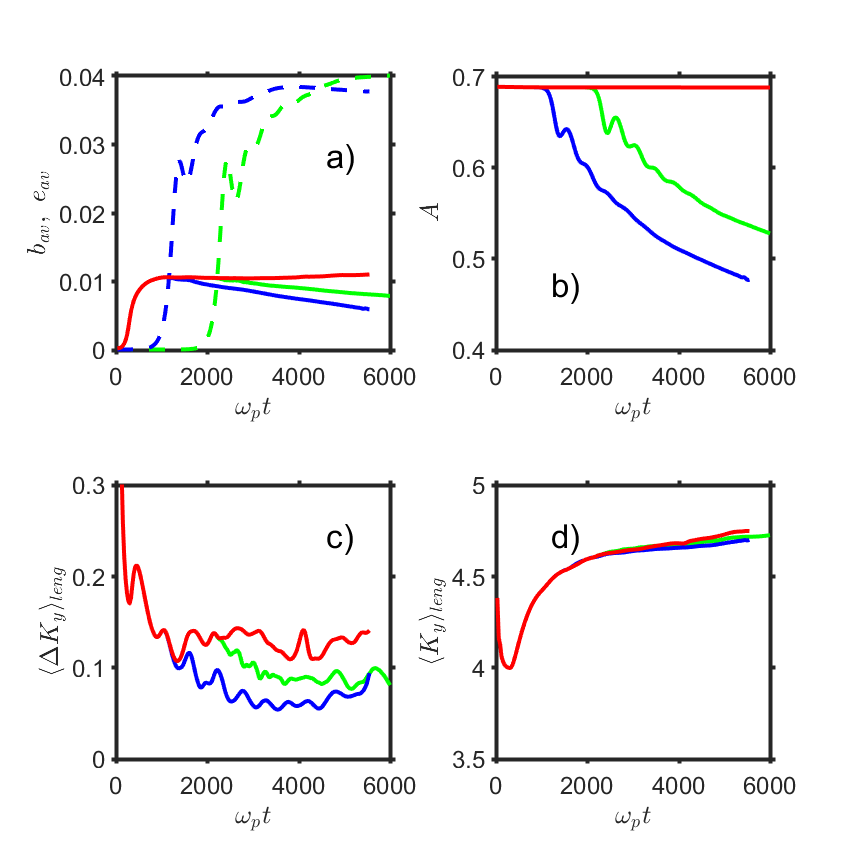
\includegraphics[width=0.5\linewidth]{part3/final_average_v2.png}
\centering
\captionstyle{normal}
\caption{Динамика (a) среднеквадратичного магнитного поля $b_{av}$ филаментационных мод (штрихи) и электрического поля $e_{av}$ двухпотоковых мод (сплошная), (b) параметра анизотропии $A$,  (c) среднеквадратичной ширины спектра ленгмюровских волн вдоль направления пучка $\langle \Delta K_y\rangle$ и (d) их среднеквадратичного продольного волнового числа $\langle K_\|\rangle$  в случае эволюции исключительно двухпотоковых мод (красный цвет) и в случае совместной эволюции двухпотоковых мод и филаментационных мод при уровнях начальных амплитуд последних, отличающихся в $10^4$ раз (синий и зеленый цвета). Параметры начального распределения (\ref{eq:bp}): $n_s=0.055n_b$, $\beta_s=2.5\beta_T$, $\beta_T=0.1$.}
\label{fig:average1}
\end{figure}

Динамика вейбелевской турбулентности, реализующейся на значительно более длинноволновых гармониках, определяется нерезонансным взаимодействием "волна-частица"~\cite{GaleevSagdeev1969,Kuznetsov2023} и слабо чувствительна к форме распределения электронов по скоростям в области резонанса с ленгмюровскими волнами. Ключевым для квазилинейного описания этой турбулентности является интегральный параметр анизотропии $A$, равный отличию от единицы отношения полной энергии электронов в продольном $W_\|$ и поперечном $W_\perp$ к скорости пучка направлении~(\ref{anisotropy}). По мере развития турбулентности распределение электронов изотропизуется, что отражается в монотонном снижении параметра анизотропии~(рис.\ref{fig:average1}b).

В рассматриваемом случае ленгмюровская турбулентность оказывается несущественной для роста флуктуаций магнитного поля и снижение параметра анизотропии диктуется исключительно вейбелевской турбулентностью. На этапе её насыщения это снижение происходит весьма быстро и достигает примерно 30\% от исходной величины $A_0=0.687$. В дальнейшем параметр анизотропии уменьшается значительно медленнее, а спектр вейбелевской турбулентности квазиавтомодельно смещается в длинноволновую область. При этом среднеквадратичное магнитное поле $b_{av}$ непосредственно после окончания экспоненциального роста демонстрирует квазистепенной рост на небольшой    промежуточной стадии, достигает максимума и далее испытывает медленное квазилинейное затухание ~(рис.\ref{fig:average1}a)~\cite{Kuznetsov2023}. В течение всего этого времени магнитная энергия на порядок и более превышает энергию квазиэлектростатического поля.

Такое поведение спектра полностью соответствует полученным ранее результатам квазилинейного подхода к эволюции бимаксвелловского распределения электронов в пределе низкой начальной анизотропии, когда среднее волновое число спектра $\langle K\rangle$ уменьшается примерно по степенному закону~\cite{Kuznetsov2023,Borodachev2016_Radiofiz} . Подобная картина наблюдалась во всех проведенных квазилинейных расчетах для системы "плазма+пучок" с небольшим начальным параметр анизотропии ($A_0\lesssim1$) и высоким уровнем достигаемой магнитной турбулентности по сравнению с ленгмюровской. 

Тем не менее, характеризуя нагрев плазмы, который в данной задаче можно связать с ростом поперечной тепловой энергии электронов $W_\perp$, следует отметить, что он является неравномерным и происходит в три этапа: 1) диссипация квазиэлектростатических полей посредством затухания Ландау в промежутке времени между достижением насыщения ленгмюровской турбулентности и началом насыщения вейбелевской, 2) преимущественная диссипация квазимагнитостатических полей, особенно эффективная в ходе их насыщения, когда амплитуды мод велики и быстро изменяются, создавая наибольшие индукционные электрические поля, 3) более медленная диссипация обоих типов квазистатических полей на временах, значительно превышающих время насыщения магнитной турбулентности. Последний этап на рис.\ref{fig:average1} не показан, а первый этап выражен слабо из-за низкого уровня развившейся ленгмюровской турбулентности. Указанные этапы нагрева имеют место и в ситуации, представленной в следующем разделе, причем там уровень ленгмюровской турбулентности выше и поэтому на первом этапе нагрев значительнее.


\section{Ослабление развития магнитной турбулентности ленгмюровскими модами}

При м\'{е}ньших, чем в предыдущем разделе, значениях скорости пучка инкремент двухпотоковых мод ослабляется и они могут развиваться одновременно с филаментационными модами. Однако тогда последние по-прежнему значительно превышают по амплитуде и подавляют первые, тем более не чувствуя наличие очень слабой ленгмюровской турбулентности. Поэтому обратимся к анализу случая б\'{о}льшего, чем в предыдущем разделе, значения скорости пучка, когда достижимы условия, в которых влияние ленгмюровской турбулентности на филаментационные моды существенно, а вклад той и другой турбулентности в изотропизацию распределения электронов по скоростям, т.е. в уменьшение параметра $A$, оказывается сопоставим.

Именно, примем для пучка примерно вдвое б\'{о}льшую направленную скорость и на порядок меньшую концентрацию частиц $n_s=0.005n_b$, $\beta_s=4\beta_T$, сохраняя небольшую начальную анизотропию $A_0=0.16$ и не слишком большой инкремент двухпотоковых мод, примерно лишь на порядок превосходящий инкремент филаментационных. Согласно~(рис. \ref{fig:average_v4}), как и в предыдущем случае, двухпотоковая неустойчивость раньше достигает насыщения, так как инкремент наиболее неустойчивой моды с продольным волновым числом $K_y\approx 3.2$ суть $\gamma_{L}\approx0.027\omega_p$, в то время как наиболее неустойчивая поперечная филаментационная мода с волновым числом $K_x\approx 0.226$ имеет инкремент $\gamma_W\approx1.27*10^{-3}\omega_p$. В результате формирующаяся ленгмюровская турбулентность деформируют распределение электронов по скоростям в области между фоновой плазмой и пучком (рис.~\ref{fig:fr2}), так что квазилинейные инкременты филаментационных мод заметно понижаются, а уровень насыщения среднеквадратичного магнитного поля вейбелевской турбулентности уменьшается примерно вдвое~(рис. \ref{fig:average_v4}a). Вместе с тем такие спектральные характеристики как среднее волновое число $\langle K\rangle$ и поперечная  $\langle\Delta K_x\rangle$  и продольная $\langle \Delta K_y\rangle$ ширина вейбелевского спектра почти не подвержены влиянию ленгмюровской турбулентности и отличаются не более чем на 1-2\% в расчетах с добавлением двухпотоковых мод и без них. 

\begin{figure}[h]
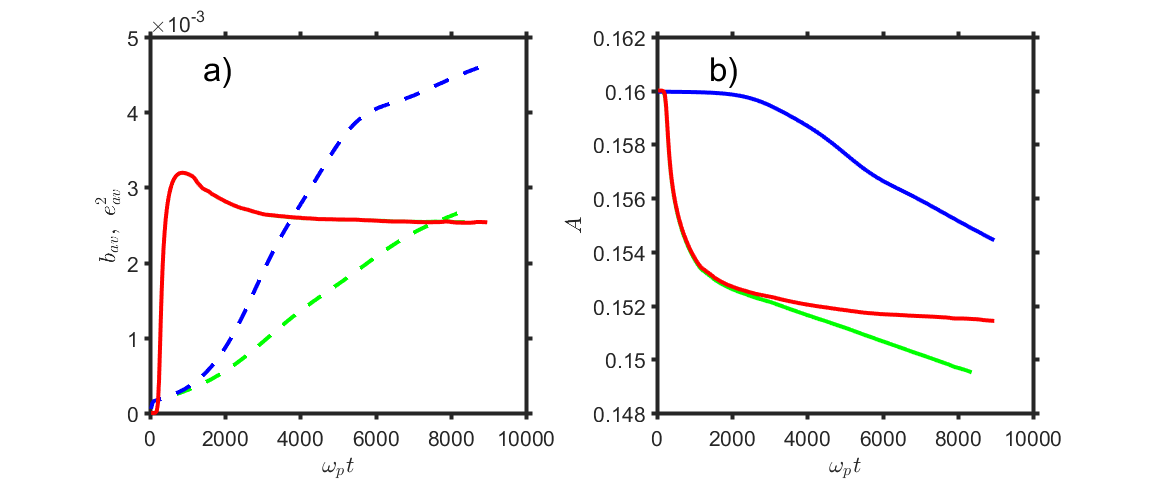
\includegraphics[width=0.7\linewidth]{part3/average_v4.png}
\centering
\captionstyle{normal}
\caption{Динамика (a) среднеквадратичного магнитного поля $b_{av}$ филаментационных мод (штрихи) и среднего квадрата электрического поля $e_{av}^2$ двухпотоковых мод (сплошная), а также (b) параметра анизотропии $A$ в случае эволюции исключительно двухпотоковых (красный цвет) либо филаментационных (синий цвет) мод и в случае их совместной эволюции (зеленый цвет). Параметры начального распределения (\ref{eq:bp}): $n_s=0.005n_b$, $\beta_s=4\beta_T$, $\beta_T=0.1$.} 
\label{fig:average_v4}
\end{figure}

На рассматриваемом промежутке времени дополнительная изотропизация распределения электронов филаментационными модами происходит преимущественно за пределами резонансной с ленгмюровскими волнами области скоростей~(рис.~\ref{fig:fr2}) и фактически начинается только при переходе на стадию насыщения вейбелевской турбулентности при $\omega_p  t > 5000$ (ср. красную и зеленую кривые для параметра анизотропии на рис. \ref{fig:average_v4}b). В результате в расчетах с добавлением филаментационных мод и без них динамика ленгмюровской турбулентности, а именно, её среднеквадратичного электрического поля, характерного волнового числа, поперечной и продольной ширины спектра не отличалась более чем на 10\%. Сказанное не исключает необходимости учета филаментационных мод при анализе затухания ленгмюровских волн на б\'{о}льших временах, на которых, однако, квазилинейное описание может оказаться некорректным из-за нарушения условий его применимости, например, вследствие накопления эффектов нелинейного трёх- или четырёхволнового взаимодействия между отдельными модами.


\begin{figure}[h]
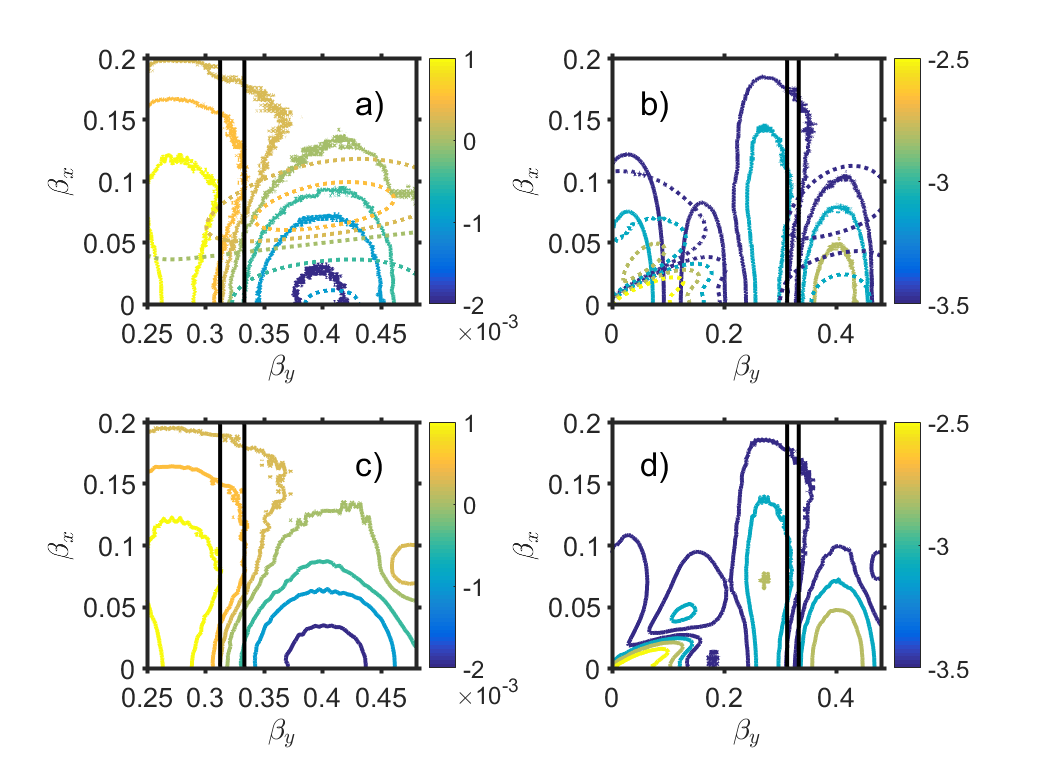
\includegraphics[width=1\linewidth]{part3/fr2.png}
\centering
\captionstyle{normal}
\caption{(a) Вычисленные для момента времени $\omega_pt=8100$ линии уровня нормированной на максимум начального распределения поправки к однородной компоненте функции распределения электронов по скоростям (\ref{eq:bp}), которая в начальный момент времени являлась максвелловской с пучком, в случае учета только двухпотоковых (сплошная) или только филаментационных (пунктир) мод. Параметры начального распределения (\ref{eq:bp}): $n_s=0.005n_b$, $\beta_s=4\beta_T$, $\beta_T=0.1$. Вертикальные черные линии отражают оценку резонансной области для коллинеарных с пучком основных энергонесущих в данный момент времени ленгмюровских мод.(b) То же для десятичного логарифма поправки к однородной компоненте функции распределения. 
(c)-(d) соответствуют графикам (a)-(b) в случае совместного учета двухпотоковых и филаментационных мод.}
\label{fig:fr2}
\end{figure}

По мере дальнейшего увеличения скорости пучка $\beta_s$ уменьшение анизотропии $A$, а также подавление роста филаментационных мод за счет насыщения роста мод ленгмюровского типа становится более значительным. Так, для параметров начального распределения $n_s=0.03n_b$, $\beta_s=5\beta_T$, $\beta_T=0.1$, при которых квазилинейная теория не применима, в расчетах методом частиц в ячейках при помощи кода EPOCH~\cite{Arber2015} турбулентное магнитное поле вейбелевских мод ослабевало примерно на порядок при учете ленгмюровской турбулентности.


\section{Заключение}

Представленные результаты демонстрируют возможные сценарии квазилинейного взаимодействия эволюционирующих спектров ленгмюровской и вейбелевской турбулентности в бесстолкновительной незамагниченной нерелятивистской плазме, включающей фоновую плазму и теплый пучок, в которых начальное распределение электронов является максвелловским с одной и той же температурой, а ионы предполагаются холодными и динамически пассивными. Реализующийся сценарий зависит от величины направленной скорости пучка и отношения концентрации его частиц к концентрации частиц фоновой плазмы. 

Если эта скорость хотя бы в несколько раз превышает тепловую, то в типичных условиях даже при относительно небольшой концентрации пучка инкремент плазменных волн значительно превышает инкремент филаментационной неустойчивости и поэтому ленгмюровская турбулентность коротковолновых квазиэлектростатических полей формируется намного раньше вейбелевской  турбулентности более длинноволновых квазимагнитостатических токов. В этом случае, как показывают квазилинейные расчеты, ленгмюровская турбулентность, выполаживающая функцию распределения электронов по скоростям в области между пучком и фоновой плазмой, может заметно уменьшить величину параметра анизотропии $A$ общего распределения электронов по скоростям, а следовательно, замедлить экспоненциальный рост филаментационных мод, понизить уровень их насыщения в ходе дальнейшего развития неустойчивости и изменить эволюцию спектра. Однако ленгмюровская турбулентность не способна подавить развитие филаментационной турбулентности, хотя результирующая энергия её магнитного поля значительно, как правило многократно, уступает энергии энергии квазиэлектростатического поля ленгмюровской турбулентности. Более того, темп затухания этой турбулентности существенно ускоряется, а расширение её спектра существенно ограничивается в результате квазилинейного воздействия развитой магнитной турбулентности.

Если же направленная скорость пучка не намного превышает тепловую скорость, примерно вдвое или менее, то при относительно небольшой концентрации пучка инкремент ленгмюровских мод оказывается меньше или порядка инкремента филаментационных, так что ленгмюровская турбулентность даже не успевает развиться до уровня собственного насыщения и довольно быстро подавляется нарастающей магнитной турбулентностью. Это происходит во многом благодаря квазилинейному эффекту деформации, сглаживания функции распределения электронов в той области скоростей, где имеет место их резонанс с ленгмюровскими волнами. Иными словами, филаментационная турбулентность квазилинейным образом подавляет ленгмюровскую. 

Проведенный анализ квазилинейного взаимодействия ленгмюровской и вейбелевской турбулентности важен для выявления других механизмов взаимного влияния турбулентных спектров квазиэлектростатических и квазимагнитостатических флуктуаций в плазменно-пучковых системах. Так, в дополнение к исследованиям трехволнового и четырехволнового взаимодействия мод ленгмюровской~\cite{Kasaba2001,Ziebell2008} и вейбелевской ~\cite{Garasev2021,Kuznetsov2025} турбулентности по отдельности, интерес представляет комбинационное взаимодействие филаментационных и двухпотоковых мод. В частности, оно может оказаться существенным для процесса аномального рассеяния резонансных с ленгмюровской волной электронов на флуктуациях магнитного поля~\cite{Fleishman2013,Medvedev2017}. При больших уровнях насыщения той или иной турбулентности, когда она уже не является достаточно слабой, многообещающим является анализ конкуренции квазилинейного взаимодействия двух типов турбулентности с их нелинейным взаимодействием за счет влияния квазиэлектро- и квазимагнитостатических полей на динамику имеющихся локализованных образований, а именно, влияния флуктуаций электрического поля на токовые z-пинчи и влияние флуктуаций магнитного поля на ленгмюровские солитоны. Кроме того, особый интерес вызывает роль аномальных столкновений, обусловленных рассеянием электронов на турбулентности в бесстолкновительной плазме и тоже являющихся нелинейным механизмом изменения инкрементов ленгмюровских и филаментационных мод, а следовательно, механизмом взаимного влияния спектров той и другой турбулентности.  

Наконец, существенным фактором развития и взаимовлияния указанных турбулентных спектров являются обычно имеющееся различие температур фона и пучка и возможное наличие релятивистских частиц в них, игнорировавшиеся в настоящей работе. Так, различие температур фона и пучка допускает пространственное разделение заряда, надлежащий учет которого снижает инкремент филаментационных мод и уровень насыщения магнитной турбулентности~\cite{Tzoufras2006,Hao2008}. 
Для широкого класса релятивистских распределений частиц по скоростям наиболее неустойчивы наклонные моды, у которых угол между волновым вектором и пучком существенно отличен и от $0$, и от $90$ градусов~\cite{Bret2004,Bret2010}. Эти и другие факторы могут повлиять на квазилинейное взаимодействие различных типов турбулентности и заслуживают дальнейшего исследования. В астрофизических задачах учет тех или иных нелинейных факторов, дополняющих разработанное квазилинейное описание совместного развития ленгмюровской и вейбелевской турбулентности, определяется свойствами неравновесной магнитоактивной плазмы конкретных космических объектов и выходит за рамки настоящей работы.
           % Глава 3
\chapter{Эволюция шланговой турбулентности магнитоактивной анизотропной плазмы 
}\label{ch:ch4}


Для определенности полагается, что в начальный момент времени нормированная функция распределения электронов по скоростям $\Psi = c^3f/N_0$ имеет бимаксвелловскую форму, вытянутую вдоль оси $z$, т.е. вдоль внешнего магнитного поля:


\begin{equation}
\label{bimax}
\Psi(\vec{\beta})=\dfrac{1}{\pi^{3/2}\beta_{\perp 0}^2 \beta_{\| 0} } \exp\left(-\dfrac{\beta_x^2+\beta_y^2}{\beta_{\perp 0}^2}-\dfrac{\beta_z^2}{\beta_{\| 0}^2}\right).
\end{equation}

Здесь $\beta_{x,y,z}={v_{x,y,z}}/{c}$, т.\,е. $\vec{\beta}=\vec{v}/{c}$. Ниже используется начальное значение параметра анизотропии $A_0={\beta^2_{\| 0}}/{\beta^2_{\perp 0}}-1 > 0$, определяемое различием исходных тепловых скоростей вдоль и поперек внешнего магнитного поля. Рассматриваемая задача, хотя и является трехмерной, обладает аксиальной симметрией. Поскольку полноценные трехмерные расчеты требуют больших вычислительных затрат, целесообразно выяснить, какие параметры турбулентности и на каких временах могут быть определены из двумерных расчетов. С этой целью в работе проведено сравнение результатов расчетов в трехмерной (3D3V) и двух вариантах двумерной (2D3V) геометриях. Во всех случаях проводится динамический учет всех трех компонент скорости частиц $\vec{v}$ и зависящих от них полей.  Ограничением в двумерных расчетах являются лишь исключенные зависимости исследуемых функций либо от координаты $y$  в $(x,z)$ -- геометрии, когда магнитное поле и ось анизотропии лежат в плоскости расчета $xz$, либо от координаты $z$ в аксиальной $z$-геометрии, когда магнитное поле и ось анизотропии ортогональны плоскости расчета $xy$.  В отличие от второго варианта, когда отсутствуют наклонные к магнитному полю моды и имеется аксиальная симметрия задачи, в первом.... усложняет динамику турбулентности, описание которой в 2D3V ..... становится некорректным в сравнении с полноценным трехмерным расчетом.
 
В работе используются обезразмеренные значения времени, волнового числа и амплитуд мод магнитного поля~(\ref{eq19plus1}):
\begin{equation}
\label{eq19plus1}
   \tau=\wpl t, \
    K=\dfrac{kc}{\wpl}, \  b_{K_{n}}=\dfrac{B_{K_{n}}}{\sqrt{8\pi N T_{\|0}}},\ 
    \wpl^2=\dfrac{4\pi Ne^2}{\me},\
    T_{\|0}=\dfrac{m_ec^2\beta_{\|0}^2}{2},
\end{equation}
Температура измеряется в энергетических единицах, т.е. с учетом постоянной Больцмана $k_B$. Для описания эволюции однородной компоненты распределения частиц по скоростям $f_0(t,\overrightarrow{\beta})=\iiint\limits^{\infty}_{-\infty}f(\vec{v},\vec{r}, t) d^3\vec{r}$ вводится относительная поправка к ней и эффективный параметр анизотропии:
\begin{equation}
\label{eq19plus2}
    \delta f_{0}(t,\overrightarrow{\beta})=\frac{f_0(t,\overrightarrow{\beta})-f_0(0,\overrightarrow{\beta})}{f_0(0,0)},\ A=\frac{2\iiint\limits^{\infty}_{-\infty}\beta_z^2f_{0}(\tau,\overrightarrow{\beta}) d\beta_x d\beta_yd\beta_z}{\iiint\limits^{\infty}_{-\infty}\left(\beta_x^2+\beta_y^2\right)f_{0}(\tau,\overrightarrow{\beta}) d\beta_x d\beta_y d\beta_z}-1 .   
\end{equation}
Кроме выявления динамики указанных величин~(\ref{eq19plus2}), представленные ниже расчеты призваны выявить закономерности в эволюции турбулентных магнитных и электрических полей и плотности тока электронов, а также пространственных спектров данной турбулентности.

Ключевыми параметрами в рассматриваемой начальной задаче о магнитной турбулентности являются начальная анизотропия $A_0$ распределения электронов по скоростям и нормированное внешнее магнитное поле $b_{ext}=B_{ext}/\sqrt{8\pi N T_{\|0}}\lesssim1$, равное обратному квадратному корню из плазменного бета-параметра. Данные величины не только задают диапазон первоначально неустойчивых мод, но и определяют дальнейшую нелинейную эволюцию спектра. В отсутствие магнитного поля имеется  апериодическое нарастание лишь ТМ-мод,  магнитное поле которых ортогонально плоскости, определяемой волновым вектором и осью анизотропии. При заданной величине поперечной компоненты волнового вектора наибольшими инкрементами обладают поперечные моды, волновые вектора которых перпендикулярны к оси анизотропии. Для них диапазон неустойчивости включает волновые числа в промежутке $\left(0;\sqrt{A_0}\right)$.\cite{??} При $A_0\ll1$ максимальный инкремент (в единицах $\omega_p$) равен $\gamma_\mathrm{max}\approx 2 \beta_{\perp0} (A_0 / 3)^{3/2}$ и достигается для оптимального волнового числа $K_\mathrm{\perp opt} \approx (A_0 / 3)^{1/2}$. При $A_0 \gg 1$ имеем $\gamma_\mathrm{max} \approx \beta_{\perp0} \left( \left[ (A_0+1)/2 \right]^{1/2} - 1 \right)$ для оптимального волнового числа $K_\mathrm{\perp opt} \approx \left( \left[ (A_0+1)/2 \right]^{1/2} - 1 \right)^{1/2}$~(рис. \ref{ris:mode_coupling}a).
\begin{figure}[h]

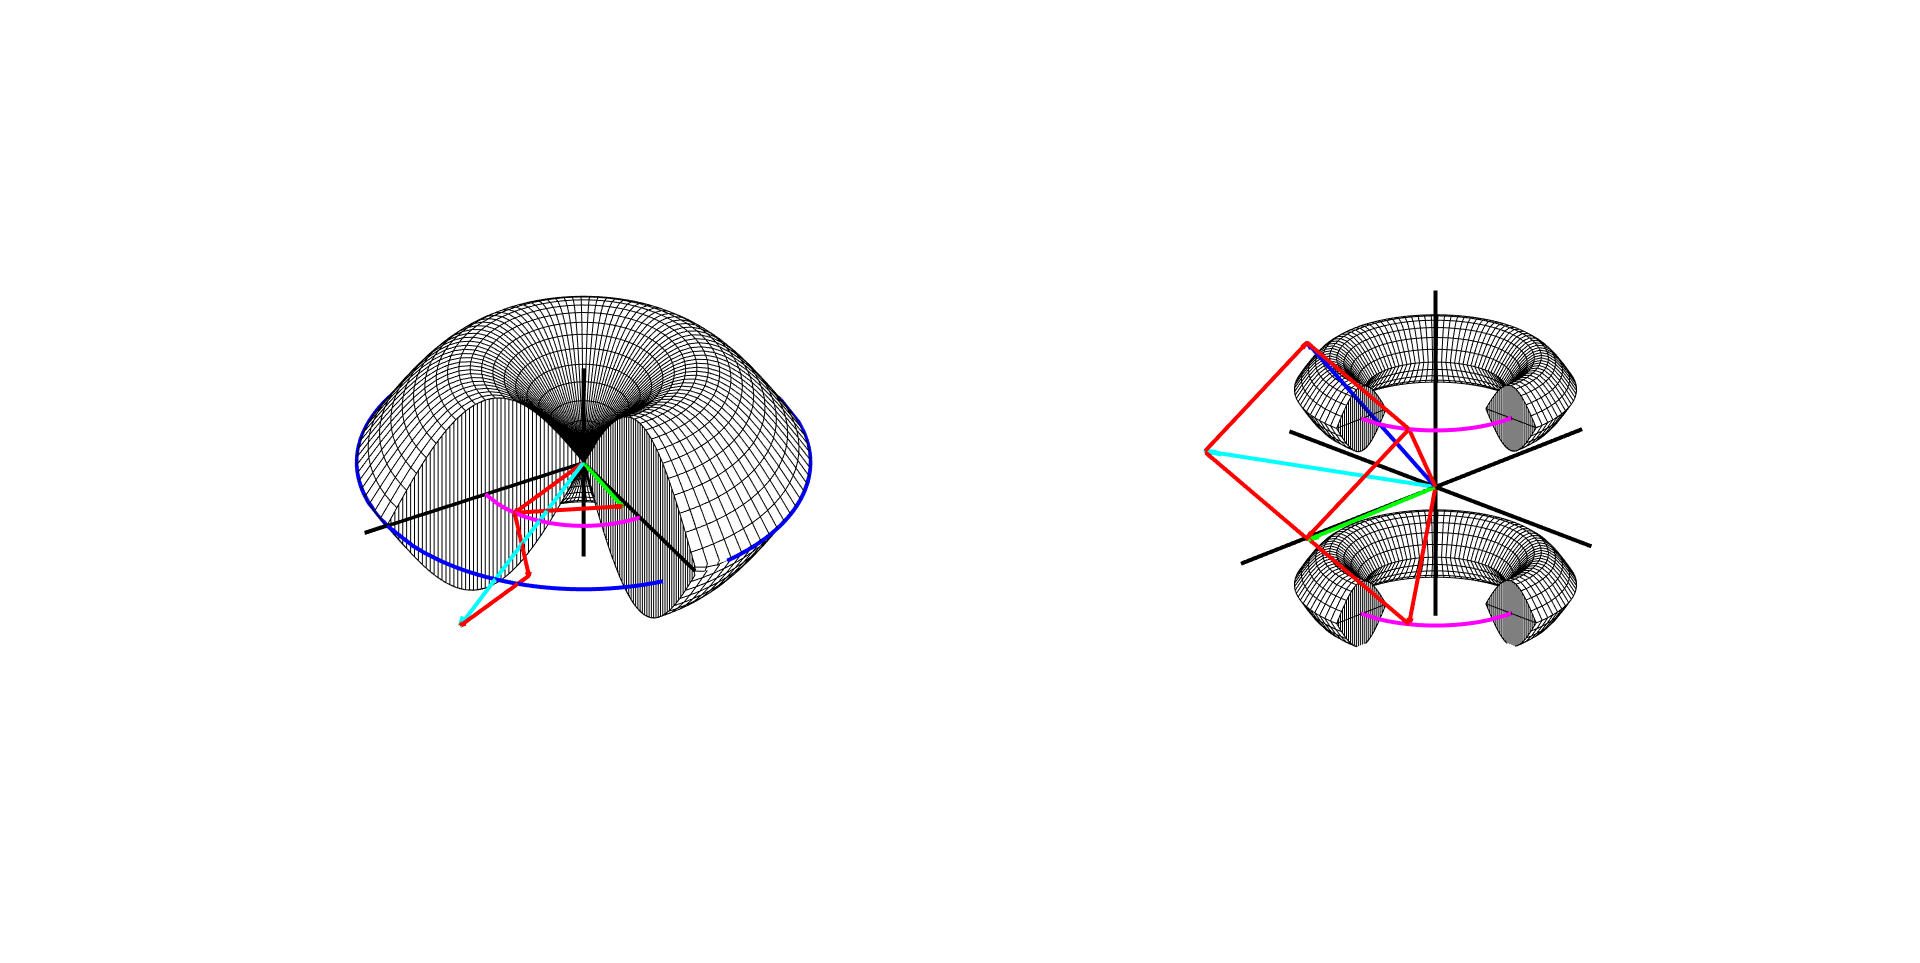
\includegraphics[width=1\linewidth]{introduction/mode_coupling.png}
\captionstyle{normal}
\caption{Трехмерная иллюстрация области апериодической неустойчивости в пространстве волновых векторов (a) в отсутствие внешнего магнитного поля и (b) в достаточно сильном внешнем магнитном поле. Синяя линия соотвествует границе неустойчивости поперечных мод $|K_\perp|=\sqrt{A}$ в отсутствие внешнего магнитного поля, а розовая линия~-- оптимальным модам $\overrightarrow{K}_{opt}$. Красные линии демонстрируют примеры оптимальных волновых векторов, взаимодействие которых в значительной степени определяет генерацию мод (зеленый, бирюзовый и синий цвет) вне области линейной неустойчивости.
}
\label{ris:mode_coupling}
\end{figure}

В присутствии внешнего магнитного поля $b_{ext}$ имеются две неустойчивые ветви: так называемые "периодическая"~ и "апериодическая"\cite{???}. Моды, направленные преимущественно вдоль внешнего магнитного поля, а значит, и оси анизотропии, относят к периодическим, поскольку их линейный инкремент мал в сравнении с действительной частотой и в сравнении с линейным инкрементом мод другой ветви~\cite{Li2000}. Поэтому влияние "периодической"~ ветви фактически не проявляется в расчетах методом частиц в ячейках, проводимых в настоящей работе, и не учитывается в приближенном квазилинейном описании.

Другую ветвь неустойчивости в литературе принято называть апериодической~\cite{???}, хотя нами показано, что в определенных условиях у ее линейно поляризованных мод присутствует действительная частота, увеличивающаяся с ростом внешнего магнитного поля $B_{ext}$ и уменьшением угла $\theta$ между волновым вектором $\vec{K}$ и этим магнитным полем. Область неустойчивости поперечных мод с увеличением внешнего поля достаточно быстро сужается,  как с длинноволновой, так и с коротковолновой стороны спектра, а линейный инкремент всех мод, остающихся неустойчивыми, уменьшается. В работе~\cite{Emelyanov2023_Radiophys} в пределе $\gamma\ll K_\perp\beta_\perp$, реализующемся при невысокой начальной анизотропии ($A_0\lesssim1$), либо при высокой анизотропии и внешнем магнитном поле, близком к подавляющему, область неустойчивости поперечных мод оценивалась как:
\begin{equation}
    K_\perp\in\left(\frac2{\sqrt{3}}\sqrt{A_0}\cos\left[\frac{\pi}3+\frac13\arccos\left(\frac{b_{ext}}{b_{s\perp}(A_0)}\right)\right];\frac2{\sqrt{3}}\sqrt{A_0}\cos\left[\frac{\pi}3-\frac13\arccos\left(\frac{b_{ext}}{b_{s\perp}(A_0)}\right)\right]\right),
    \label{eq:border_perp_inst}
\end{equation}
где $b_{s\perp}(A_0)$~--- нормированное магнитное поле, подавляющее неустойчивость поперечных мод, квадрат которого оценен в~\cite{Emelyanov2023_Radiophys} как:
\begin{equation}
    b_{s\perp}^2(A_0)=\frac{8\pi}{27}\frac{A_0^3}{1+A_0^3}<1.
    \label{eq:Emel_condition}
\end{equation}
По мере увеличения внешнего магнитного поля $b_{ext}$ монотонно уменьшается не только линейный инкремент всех поперечных мод, но и угол между внешним магнитным полем и волновым вектором моды с наибольшим инкрементом~(рис. \ref{ris:mode_coupling}b)~\cite{Moya2022,Li2000,Camporeale2008}. Таким образом, для наклонных мод неустойчивость может развиваться при $b_{ext}>b_{s\perp}(A_0)$. Вводя величину магнитного поля $b_s(A_0)$, при которой апериодическая неустойчивость полностью подавлена, приведем оценку для неё из работы~\cite{Hellinger2014}, аппроксимирующую численно полученный порог неустойчивости в диапазоне значений начальной анизотропии $A_0$ от $0.2$ до $9$:

\begin{equation}
    b_{s}^2(A_0)=\left(\frac{A_0}{1.27(1+A_0)}\right)^{\frac1{0.954}}.
    \label{eq:Hellinger_condition}
\end{equation}
\begin{figure}[h]

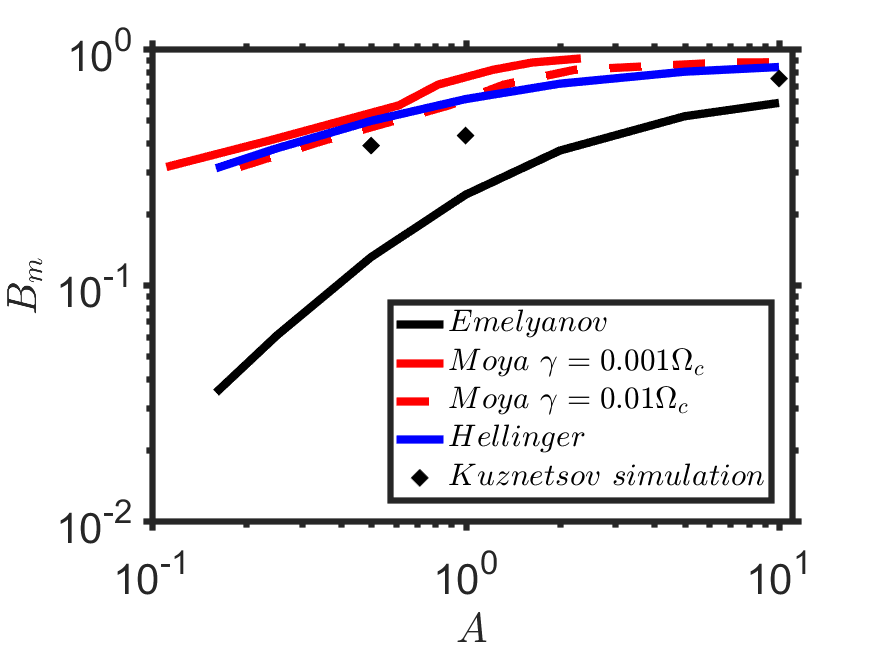
\includegraphics[width=0.5\linewidth]{introduction/b_podavl12.png}
\centering
\captionstyle{normal}
\caption{Зависимость подавляющего внешнего магнитного поля от начальной анизотропии для поперечных апериодических мод~(\ref{eq:Emel_condition}) (черный цвет), всех апериодических мод согласно оценке~(\ref{eq:Hellinger_condition}) (синий цвет) и согласно результатам расчетов~\cite{Moya2022} (красный цвет).}

\label{ris:B_podavl}
\end{figure}

Сравнение оценок (\ref{eq:Emel_condition}) и (\ref{eq:Hellinger_condition}) показывает, что если при высоких начальных анизотропиях отношение $ b_{s}^2/ b_{s\perp}^2$ лишь немного превышает единицу, то при низких начальных анизотропиях оно может составлять несколько порядков~(рис. \ref{ris:B_podavl}). Значит, существует широкий диапазон параметров, в котором принципиально важен учет наклонных мод, так как поперечные моды устойчивы в линейном приближении.

\section{Деформация распределения частиц в зависимости от величины  внешнего магнитного поля}
\label{part_evol_distr_func}
В отсутствии внешнего магнитного поля и наклонных мод ранее наблюдалась значительная деформация функции распределения частиц на стадии насыщения экспоненциального роста во всей области скоростей порядка тепловых~\cite{Kuznetsov2023}. В данном процессе происходит быстрое увеличение поперечной к оси анизотропии скорости электронов, двигавшихся сначала преимущественно вдоль этой оси, так что его форма принимает вид, существенно отличный от бимаксвелловского~(рис. \ref{ris:FR_A10_3d_B0}). В дальнейшем форма функции распределения частиц, остающаяся сильно не бимаксвелловской, изменяется медленно, квазилинейно, т.е. исключительно за счет интегрального нелинейного влияния мод на однородную компоненту функции распределения в условиях формально линейной эволюции каждой моды согласно текущему значению инкремента (декремента) и частоты (в общем случае ненулевой), определяемыми этой медленно меняющейся функцией распределения частиц. Это было показано сравнением симуляций методом частиц в ячейках с расчетами, учитывающими исключительно квазилинейное взаимодействие. На временах, по меньшей мере пятикратно превышающих момент окончания экспоненциального роста, учет наклонных мод и нелинейных взаимодействий, с ними связанных, в отсутствие внешнего магнитного поля не оказывает существенного влияния на эволюцию распределения частиц по скоростям за исключением, возможно, кратковременного переходного промежутка примерно от $\omega_pt=80$ до $\omega_pt=100$ при насыщении неустойчивости. 


\begin{figure}[h!]
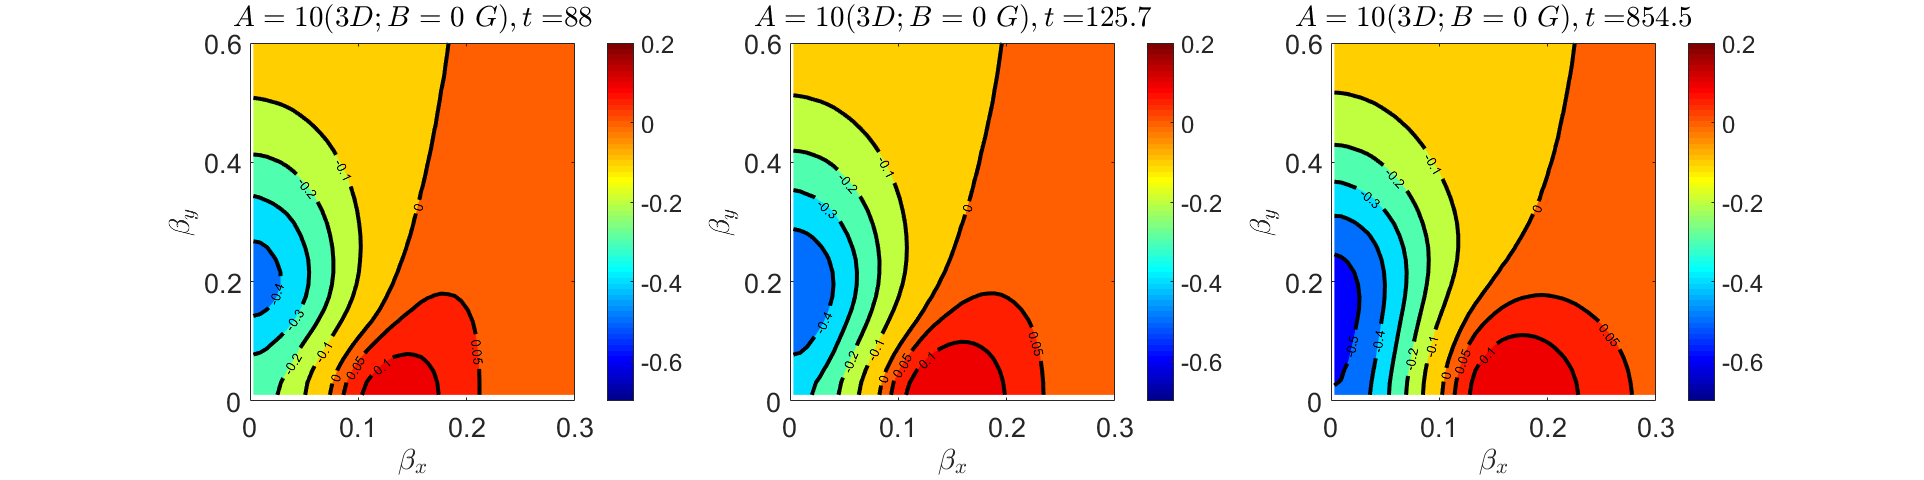
\includegraphics[width=1\linewidth]{part4/FR_B0_A10_3d.png}
\captionstyle{normal}
\caption{Вычисленные для моментов времени (a)~$\wpl t = 88$, (b)~$\wpl t = 125.7$, (c)~$\wpl t = 854.5$ линии уровня $-0.5$, $-0.4$, $-0.3$, $-0.2$, $-0.1$, $0$, $0.05$ и $0.1$ нормированной на максимум начального распределения поправки к однородной компоненте функции распределения (\ref{bimax}), которая в начальный момент времени являлась бимаксвелловской с параметром анизотропии $A_0=10$. Внешнее магнитное поле отсутствует: $b_{ext}=0$.}
\label{ris:FR_A10_3d_B0}
\end{figure}


В присутствии внешнего магнитного поля, по-прежнему, при насыщении неустойчивости происходит сравнительно быстрое увеличение поперечной к оси анизотропии скорости электронов, двигавшихся сначала преимущественно вдоль этой оси. С увеличением внешнего магнитного поля количество таких электронов уменьшается,  продольная скорость области их наибольшего прироста в момент насыщения неустойчивости увеличивается от нуля до $\beta_\|\sim3\beta_{\perp0}$, а поперечная остается примерно неизменной $\beta_\perp\lesssim2\beta_{\perp0}$ (рис. ~\ref{ris:FR_A10_3d_B78}). В ходе дальнейшего нелинейного развития турбулентности в отсутствие внешнего магнитного поля форма ФР частиц по скоростям меняется слабо, преимущественно за счет нагрева в поперечном к оси анизотропии направлении электронов с малой продольной скоростью, что расширяет область значительного оттока частиц в диапазон малых скоростей $\left(\beta_\perp<\beta_{\perp0},\beta_\|<\beta_{\|0}\right)$ (рис. \ref{ris:FR_A10_3d_B44}). Посредством сравнения трехмерных и двумерных аксиально симметричных расчетов кодом EPOCH с квазилинейным моделированием, в котором исключено прямое нелинейное взаимодействие между модами и оставлено лишь квазилинейное взаимодействие, было выявлено, что хотя к моменту насыщения неустойчивости указанные распределения частиц аналогичны, на более поздних временах они качественно отличаются в диапазоне малых скоростей  (ср. рис. \ref{ris:FR_A10_3d_B44_QL} и рис. \ref{ris:FR_A10_3d_B44}). Эта разница определяется существенно отличной динамикой спектра в обсуждаемых симуляциях (см. раздел \ref{part_spectr_b4}). Из этих различий следует, что квазилинейное приближение недостаточно для описания эволюции турбулентности  уже при довольно слабом внешнем магнитном поле, например, $b_{ext}=0.4$ при $A_0=10$. 

\begin{figure}[h!]
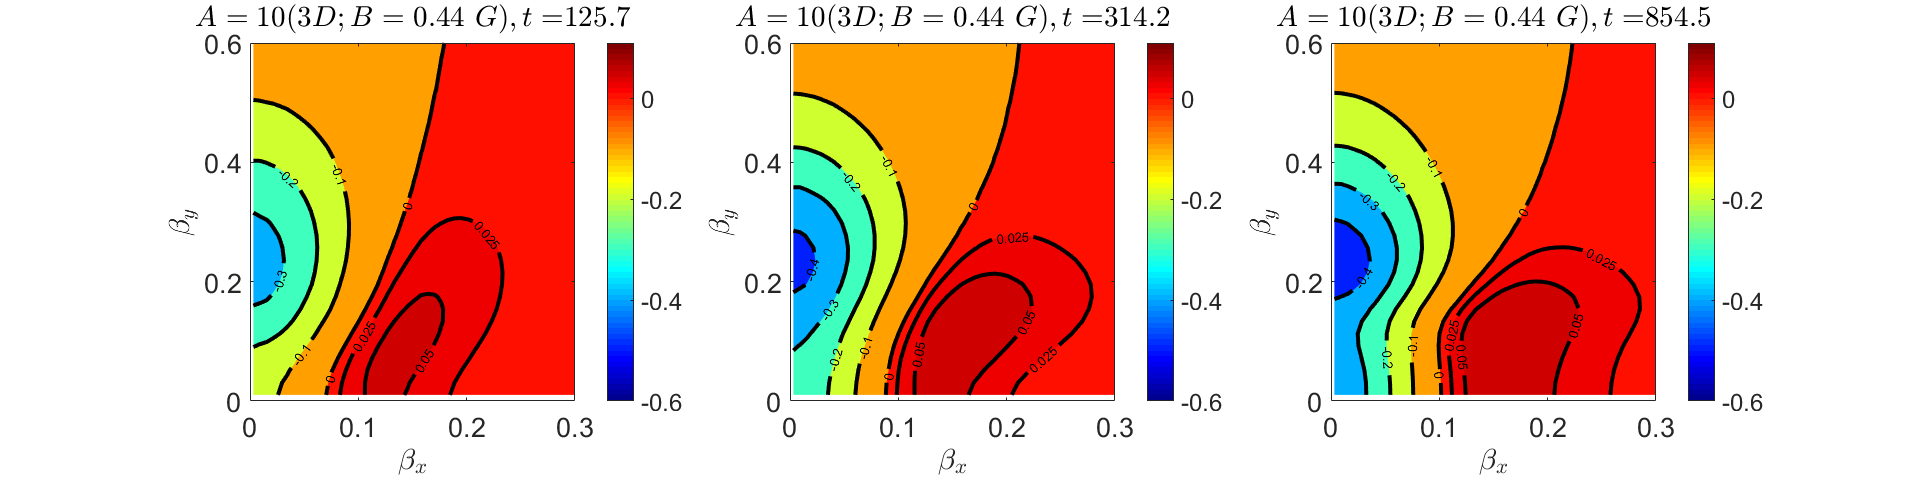
\includegraphics[width=1\linewidth]{part4/FR_B044_A10_3d.png}
\captionstyle{normal}
\caption{Вычисленные для моментов времени (a)~$\wpl t = 125.7$, (b)~$\wpl t = 314.2$, (c)~$\wpl t = 854.5$ линии уровня $-0.4$, $-0.3$, $-0.2$, $-0.1$, $0$, $0.025$ и $0.05$ нормированной на максимум начального распределения поправки к однородной компоненте функции распределения (\ref{bimax}), которая в начальный момент времени являлась бимаксвелловской с параметром анизотропии $A_0=10$. Внешнее магнитное поле $b_{ext}=0.4$.}
\label{ris:FR_A10_3d_B44}
\end{figure}

\begin{figure}[h!]

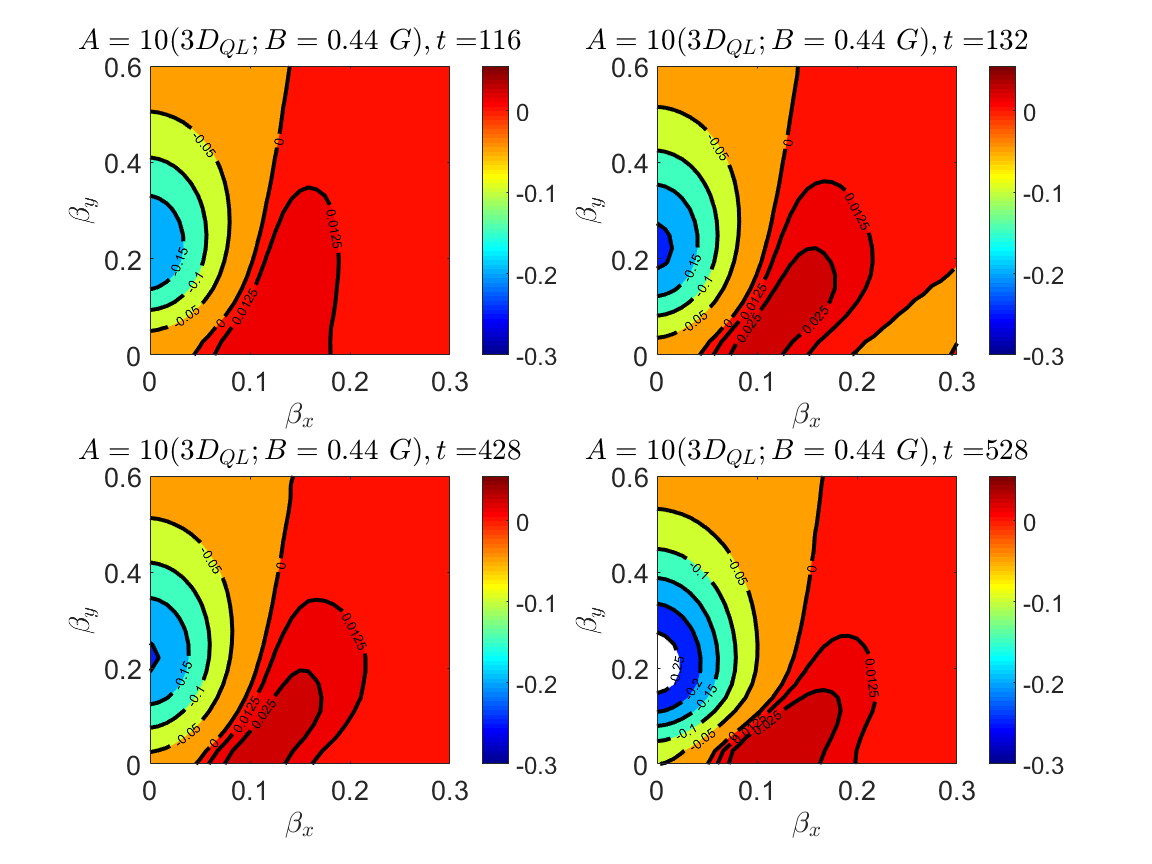
\includegraphics[width=1\linewidth]{part4/FR_QL_B4_A10.png}
\captionstyle{normal}
\caption{Вычисленные в квазилинейном аксиально симметричном приближении~\cite{Kuznetsov2023} для моментов времени (a)~$\wpl t = 84$, (b)~$\wpl t = 92$, (c)~$\wpl t = 100$, (d)~$\wpl t = 420$ линии уровня $-0.5$, $-0.4$, $-0.3$, $-0.2$, $-0.1$, $0$, $0.05$ и $0.1$ нормированной на максимум начального распределения поправки к однородной компоненте функции распределения (\ref{bimax}), которая в начальный момент времени являлась бимаксвелловской с параметром анизотропии $A_0=10$. Внешнее магнитное поле $b_{ext}=0.4$.}
\label{ris:FR_A10_3d_B44_QL}
\end{figure}

Нелинейное долговременное изменение ФР становится всё более заметным с увеличением магнитного поля: при $b_{ext}=0.71$ деформация ФР происходит преимущественно значительно позднее насыщения линейной апериодической неустойчивости. Продольная скорость расширяющейся области  наибольшего прироста снижается с $\beta_\|\sim3\beta_{\perp0}$ до $\beta_\|\sim2\beta_{\perp0}$, а поперечная почти не меняется.  Область значительного оттока частиц, абсолютный максимум которого достигается при $\beta_\|\sim3\beta_{\perp0}$,  также существенно расширяется на нелинейной стадии, причем появляется локальный максимум в области малых скоростей $\left(\beta_\perp<\beta_{\perp0},\beta_\|<\beta_{\|0}\right)$.
\begin{figure}[h!]

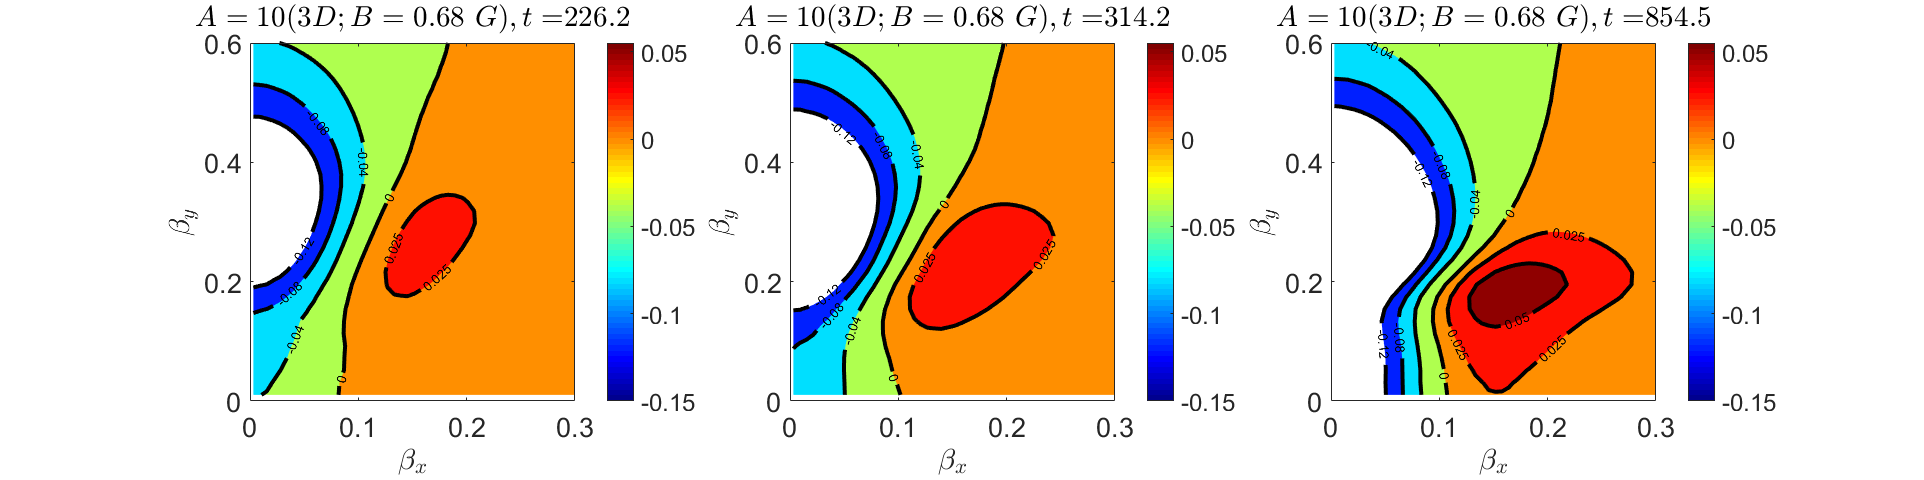
\includegraphics[width=1\linewidth]{part4/FR_B065_A10_3d.png}
\captionstyle{normal}
\caption{Вычисленные для моментов времени (a)~$\wpl t = 226.2$, (b)~$\wpl t = 314.2$, (c)~$\wpl t = 854.5$ линии уровня $-0.4$, $-0.3$, $-0.2$, $-0.1$, $0$, $0.025$ и $0.05$ нормированной на максимум начального распределения поправки к однородной компоненте функции распределения (\ref{bimax}), которая в начальный момент времени являлась бимаксвелловской с параметром анизотропии $A_0=10$. Внешнее магнитное поле $b_{ext}=0.59$.}
\label{ris:FR_A10_3d_B65}
\end{figure}


\begin{figure}[h!]
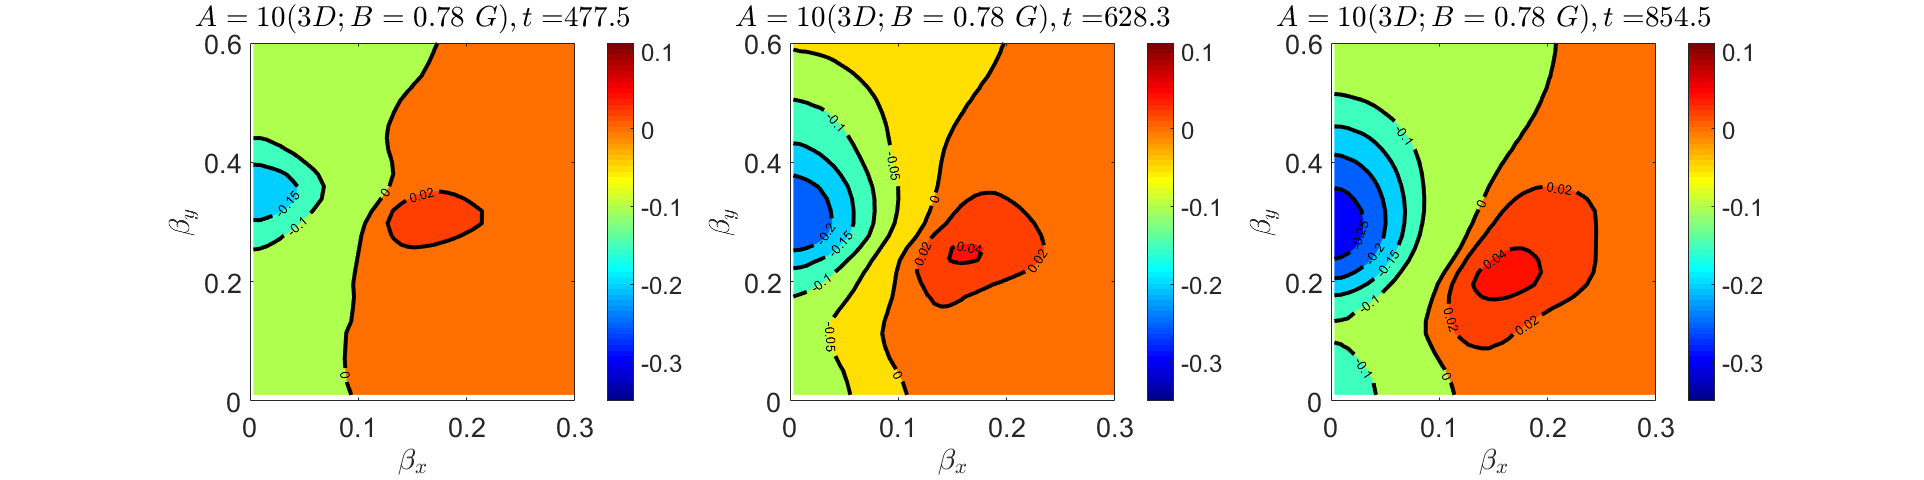
\includegraphics[width=1\linewidth]{part4/FR_B078_A10_3d.png}
\captionstyle{normal}
\caption{Вычисленные для моментов времени (a)~$\wpl t = 477.5$, (b)~$\wpl t = 628.3$, (c)~$\wpl t = 854.5$ линии уровня $-0.25$, $-0.2$, $-0.15$, $-0.1$, $-0.05$, $0$, $0.02$ и $0.04$ нормированной на максимум начального распределения поправки к однородной компоненте функции распределения (\ref{bimax}), которая в начальный момент времени являлась бимаксвелловской с параметром анизотропии $A_0=10$. Внешнее магнитное поле $b_{ext}=0.71$.}
\label{ris:FR_A10_3d_B78}
\end{figure}

Функции распределения частиц по скоростям в двумерных расчетах 2D3V с магнитным полем, лежащим в плоскости моделирования, демонстрируют качественно схожую динамику. Наиболее значительные отличия наблюдаются в отсутствие внешнего магнитного поля:  ФР в 2D3V-расчете теряет аксиальную симметрию, изотропизуясь лишь в плоскости, ортогональной к перпендикулярным волновым векторам. В присутствии внешнего магнитного поля распределение частиц испытывает ларморовское вращение и посредством этого приобретает возможность изотропизоваться в обоих перпендикулярных к оси анизотропии направлениях, стремясь, что особенно ярко выражено в сильном внешнем магнитном поле, к аксиально симметричному виду, аналогичному распределению частиц в трехмерных симуляциях. 


\section{Эволюция интегральных характеристик турбулентности при различных значениях внешнего магнитного поля}
\label{part_evol_aver}


Параметр анизотропии $A$, будучи интегральным отражением формы распределения частиц, в отсутствие внешнего магнитного поля испытывает наиболее значительное снижение к моменту насыщения неустойчивости, а в сильном магнитном поле, равном, например, $b_{ext}=0.71$, ситуация противоположная и изотропизация распределения происходит преимущественно в ходе нелинейной эволюции (рис. \ref{ris:average_A10}b). Так, в первом случае к насыщению неустойчивости в $\tau_s=88$ анизотропия резко, примерно в 5 раз, уменьшается до $\approx2$, далее её снижение плавно замедляется и на временах $2\tau_s=176$ она составляет $A\approx1.1$. Во втором случае к моменту насыщения неустойчивости $\tau_s=390$ анизотропия снижается всего до $\approx7.2$, а на временах $2\tau_s=780$ составляет уже $A\approx3.83$.

Тем интереснее, что величина среднеквадратичного магнитного поля к концу симуляции в этих противоположных случаях различалась всего на $5 \%$ (рис. \ref{ris:average_A10}a,d). В отсутствие внешнего поля эта величина сравнительно быстро выросла, достигла насыщения и начала быстро затухать. В сильном же внешнем поле апериодическая неустойчивость достигла своего насыщения в $4$ раза позднее и при в $3.5$ раза меньшем турбулентном магнитном поле, однако после этого  среднеквадратичное магнитное поле до конца симуляции находилось на примерно одном и том же уровне, что предопределило близость обсуждаемых величин к концу обеих симуляций. Полученное совпадение не выглядит случайным, так как среднеквадратичное магнитное поле в двух других расчетах с промежуточными значениями магнитного поля $b_{ext}=0.4$ и $b_{ext}=0.59$ к концу симуляции пришло к сравнимым значениям, отличающимся всего на $10 \%$ и $20 \%$ соответственно. Идентичный результат наблюдается и для аналогичных симуляций при начальной анизотропии $A_0=1$. Это позволяет предполагать, что внешнее магнитное поле, неизбежно присутствующее в корональных петлях, хотя и существенно меняет динамику турбулентного магнитного поля непосредственно после насыщения неустойчивости, слабо влияет на среднеквадратичную величину последнего на глубоко нелинейных временах, на которых масштабы турбулентности во всех направлениях сопоставимы. 
\begin{figure}[h]
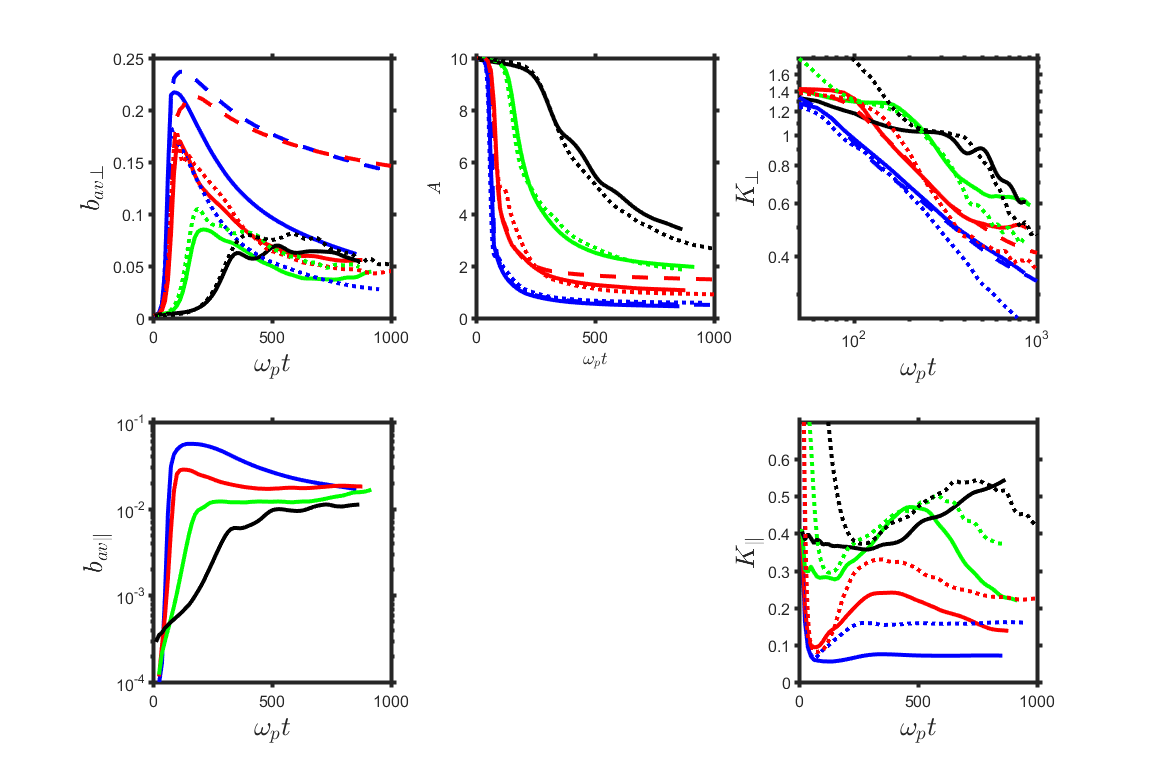
\includegraphics[width=1\linewidth]{part4/average_A10.png}
\captionstyle{normal}
\caption{Эволюция (a) поперечной и (d) продольной компонент среднеквадратичного магнитного поля $b_{av}$, (b) параметра анизотропии $A$, характерных (c) поперечной $\langle K_\perp\rangle$ и (f) продольной $\langle K_\|\rangle$ компонент волнового числа при значениях внешнего магнитного поля $b_{ext}=0$ (синий цвет), $b_{ext}=0.4$ (красный цвет), $b_{ext}=0.59$ (зеленый цвет) и $b_{ext}=0.71$ (черный цвет) в трехмерных (сплошная линия), двумерных с наклонными модами (пунктир) и двумерных аксиально симметричных (штрихи) симуляциях. Начальная анизотропия равна $A_0=10$.}
\label{ris:average_A10}
\end{figure}

Во всех трехмерных симуляциях преобладает поперечная к оси анизотропии компонента магнитного поля, кратно, но не на порядки превосходя продольную компоненту. На протяжении нелинейной эволюции турбулентности их отношение уменьшается. Так, в отсутствие внешнего магнитного поля при насыщении неустойчивости их отношение примерно равно $b_\perp/b_\|\approx4$, на момент окончания расчета~--- $b_\perp/b_\|\approx3$, а в сильном внешнем магнитном поле $b_{ext}=0.71$ при насыщении неустойчивости их отношение примерно равно $b_\perp/b_\|\approx10$,  на момент окончания расчета~--- $b_\perp/b_\|\approx5$. 

Значения характерных перпендикулярного $\langle K_\perp\rangle$ и продольного $\langle K_\|\rangle$ волновых чисел к моменту насыщения неустойчивости соответствуют волновому вектору наиболее неустойчивой моды, а значит, определяются линейной теорией. Здесь усреднение понимается в следующем смысле:
\begin{equation}
\label{eq:angles}
\langle...\rangle=\frac{\iiint\limits_0^\infty...b_K^2 d^3K}{\iiint\limits_0^\infty b_K^2 d^3K} ,
\end{equation}
Первое увеличивается c ростом внешнего магнитного поля, пока наиболее неустойчивыми модами остаются поперечные моды. При дальнейшем увеличении внешнего магнитного поля определяющими всю динамику турбулентности становятся наклонные моды, а характерное перпендикулярное волновое число снижается. Характерное продольное волновое число $\langle K_\|\rangle$в момент насыщения неустойчивости с ростом внешнего магнитного поля увеличивается.

В ходе последующей нелинейной эволюции поперечный масштаб турбулентности практически монотонно возрастает (рис. \ref{ris:average_A10}с и рис. \ref{ris:average_A10}f). Продольный масштаб сначала убывает вследствие нелинейного возбуждения разнообразных наклонных мод, устойчивых согласно линейной теории, а затем тоже возрастает. К концу симуляции во всех случаях продольный и поперечный масштабы оказывались сопоставимы, так что становится невозможно говорить о филаментационной структуре токов. В целом, результаты согласуются с~\cite{Hellinger2014,Camporeale2008}, отмечавшими увеличение масштаба турбулентности и уменьшение угла между внешним магнитным полем и характерным волновым вектором. Несмотря на хорошее количественное совпадение для всех четырех значений внешнего магнитного поля результатов эволюции параметра анизотропии (точность до 15\%) и среднеквадратичного магнитного поля (без случая $b_{ext}=0$ точность до 20 \%) у двумерных и трехмерных расчетов, сравнение в этих расчетах продольного и поперечного характерных масштабов турбулентности показывает, что на нелинейной стадии они значительно расходятся и могут кратно отличаться.  Это существенно затрудняет изучение долговременной спектральной эволюции трехмерной турбулентности на основе анализа двумерных симуляций, как это, по-видимому, делается в указанных выше работах. Анализ спектральной динамики турбулентности, генерируемой шланговой модой, ниже основан на трехмерных симуляциях и посвящен преимущественно спектральной динамике поперечной компоненты магнитного поля, усредненной по аксильному углу. Усреднение приводит к сглаживанию шумов и осцилляций, наблюдаемых на стадии затухания мод, что позволяет оценить показатель степенного спадания их амплитуды.

\section{Влияние внешнего магнитного поля на спектральную эволюцию шланговой турбулентности и нелинейные эффекты четырехволнового и трехволнового взаимодействия мод}
\subsection{Динамика спектра вейбелевской турбулентности и нелинейное взаимодействие мод в отсутствие внешнего магнитного поля}
\label{part_spectr_bo}


В отсутствие наклонных мод и внешнего магнитного поля общий сценарий эволюции спектра вейбелевской турбулентности, который по существу можно назвать квазилинейным, был подробно описан в работе~\cite{Kuznetsov2023} в аксиально симметричной двумерной геометрии (все моды лежат в плоскости, ортогональной к оси анизотропии). При бимаксвелловском начальном распределении частиц неустойчивой оказывается исключительно ТМ-мода, магнитное поле которой ортогонально к плоскости опредлеляемой осью анизотропии и волновым вектором. После насыщения неустойчивости спектр магнитного поля, управляемый преимущественно квазилинейным взаимодействием, смещается в длинноволновую область так, что характерное волновое число уменьшается степенным образом, а степень наклона длинноволнового и коротковолнового хвостов остается при.
мерно постоянной, что говорит об автомодельности динамики спектра. Единственным наблюдаемым нелинейным эффектом является развитие ТМ-гармоник, нечетным образом кратных к оптимальной, преимущественно утроенной гармоники, генерируемой четырехволновым взаимодействием~\cite{Garasev2021,Kuznetsov2023}. Таким образом, были выделены 4 стадии эволюции ТМ-мод: экспоненциальный рост согласно линейному дисперсионному уравнению, степенной рост мод, волновое число которых меньше характерного $\langle K_\perp\rangle$, осцилляционное затухание мод, волновое число которых больше характерного $\langle K_\perp\rangle$, и сверхбыстрый нелинейный рост вследствие четырехволнового взаимодействия~(рис. \ref{ris:all_modes}a).  Показатель степенного роста оценивался примерно от $1$ до $2$, а показатель затухания, которое после усреднения по аксиальному углу оказывалось степенным, лежал в небольшом диапазоне значений от $-1.3$ до $-1$ для широкого диапазона значений начальных анизотропий. 

\begin{figure}[h]
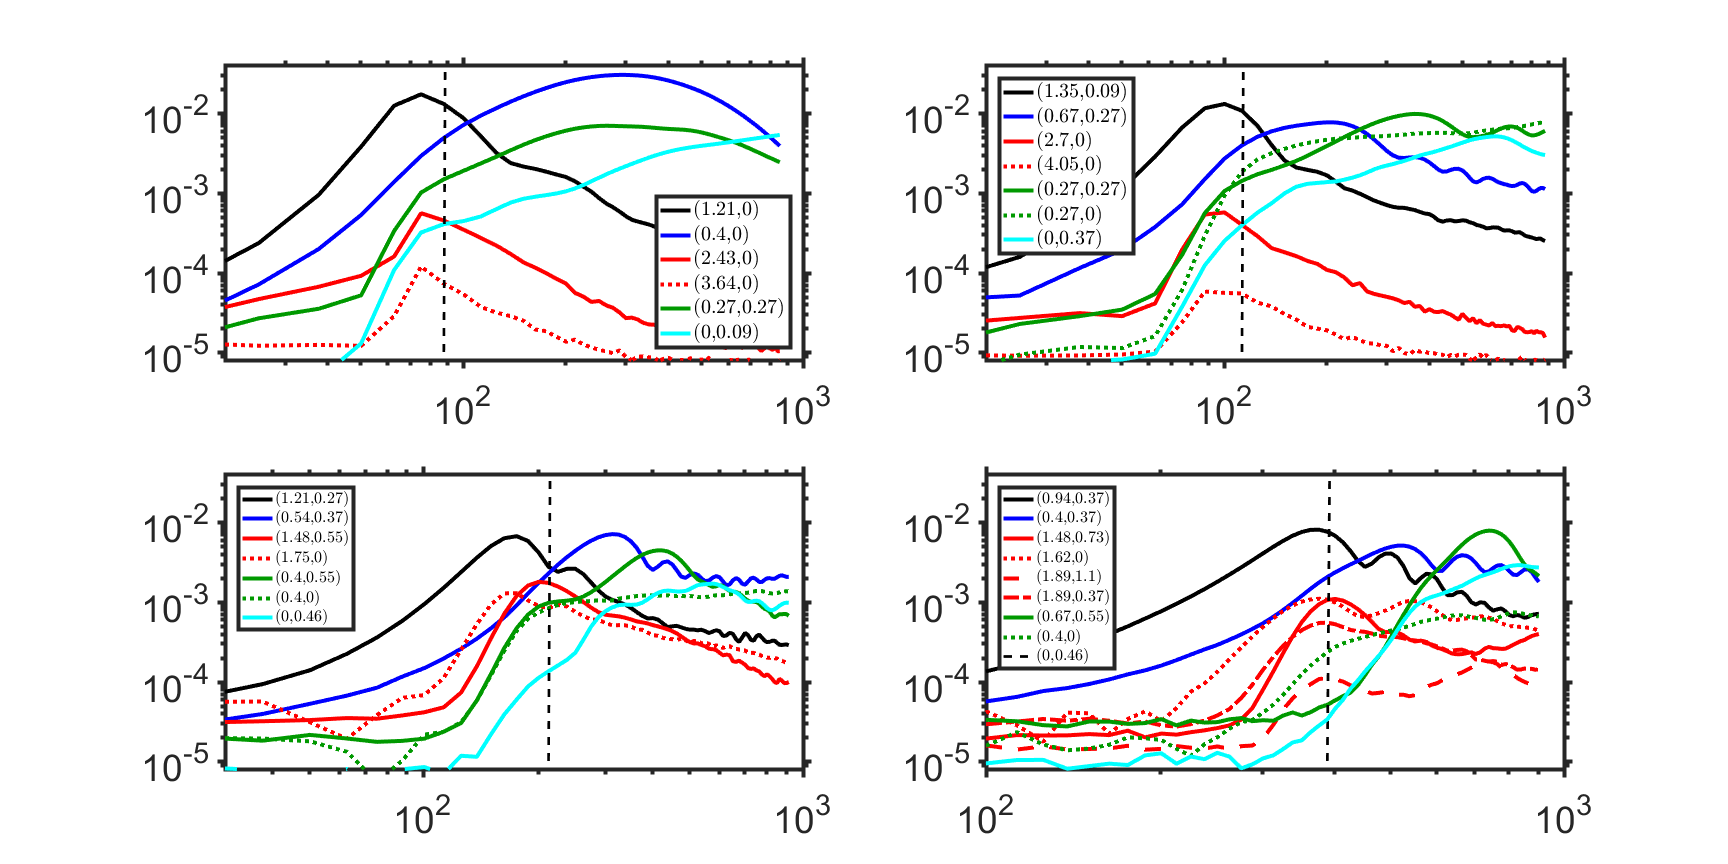
\includegraphics[width=1\linewidth]{part4/garmoniki_final.png}
\captionstyle{normal}
\caption{Эволюция типичных усредненных по аксиальному углу мод: примерно оптимальной моды $\overrightarrow{K}_{opt}$ (черный цвет); линейно неустойчивой моды, испытывающей степенное нарастание (синий цвет);  линейно устойчивых, затухающих непосредственно после сверхбыстрой генерации мод (красный цвет); линейно устойчивых, примерно степенным образом нарастающих после окончания сверхбыстрой генерации мод (зеленый цвет), наиболее энергонесущей моды с $K_\perp=0$ (бирюзовый цвет) при внешнем магнитном поле (a) $b_{ext}=0$, (b) $b_{ext}=0.4$. (c) $b_{ext}=0.59$, (d) $b_{ext}=0.71$. Вертикальный пунктир соответствует первому локальному максимуму среднеквадратичного магнитного поля в каждом случае. Начальная анизотропия $A_0=10$.}
\label{ris:all_modes}
\end{figure}

Другим нелинейным эффектом, который наблюдается в аксиально симметричной двумерной (как в работе \cite{Kuznetsov2023}) и трехмерной (3D3V) геометриях, является трехволновая генерация линейно устойчивых ТЕ-мод, т.е. мод, электрическое поле которых ортогонально к плоскости, определяемой волновым вектором и осью анизотропиии, посредством взаимодействия двух апериодических неустойчивых ТМ-мод~(см. рис. \ref{ris:mode_coupling}a). Этот эффект проявляется на стадии линейной неустойчивости в экспоненциальном росте ТЕ-мод с инкрементом, меньшим или порядка удвоенного максимального (точной оценке препятствует высокий уровень шумов). Область наблюдаемой генерации волновых чисел ТЕ-мод сравнима с областью линейно неустойчивых мод, а оптимальная ТЕ-мода немного смещена в длинноволновую область относительно оптимальной ТМ-моды ($\approx20-30\%$). В двумерной (2D3V) геометрии (как в работах~\cite{Camporeale2008,Hellinger2014}) с наклонными модами подобное взаимодействие геометрически невозможно, поэтому продольная компонента магнитного поля отсутствует. 



Добавление наклонных мод еще сильнее увеличивает разнообразие и влияние нелинейных взаимодействий, из-за которых наблюдается нелинейный сверхбыстрый рост не только поперечных ТМ-мод коротковолнового крыла, но и широкого разнообразия наклонных ТМ-мод, инкремент которых, согласно линейной теории для текущего распределения частиц, близок к нулю или вовсе отрицателен~(рис. \ref{ris:spectrA10_B0}). Хотя квазилинейное взаимодействие, по-видимому, продолжает играть важную роль, спектральная динамика существенно перестает быть квазилинейной: спектр турбулентности за счет прямых нелинейных взаимодействий между гармониками расширяется вдоль оси анизотропии, а среднеквадратичное магнитное поле затухает значительно быстрее, чем в аксиально симметричных расчетах без учета наклонных мод. Мы предполагаем, что приблизить результаты квазилинейных расчетов к результатам трехмерных симуляций методом частиц в ячейках если не в переходной области после насыщения неустойчивости, то хотя бы на глубоко нелинейной стадии развития может ввод аномальной частоты столкновений в БГК-приближении~\cite{Bhatnagar1954,Medvedev2017}, эффективно описывающих нелинейные взаимодействия между модами магнитного поля и распределения частиц. Эта возможность станет предметом дальнейших исследований.

\begin{figure}[h] 
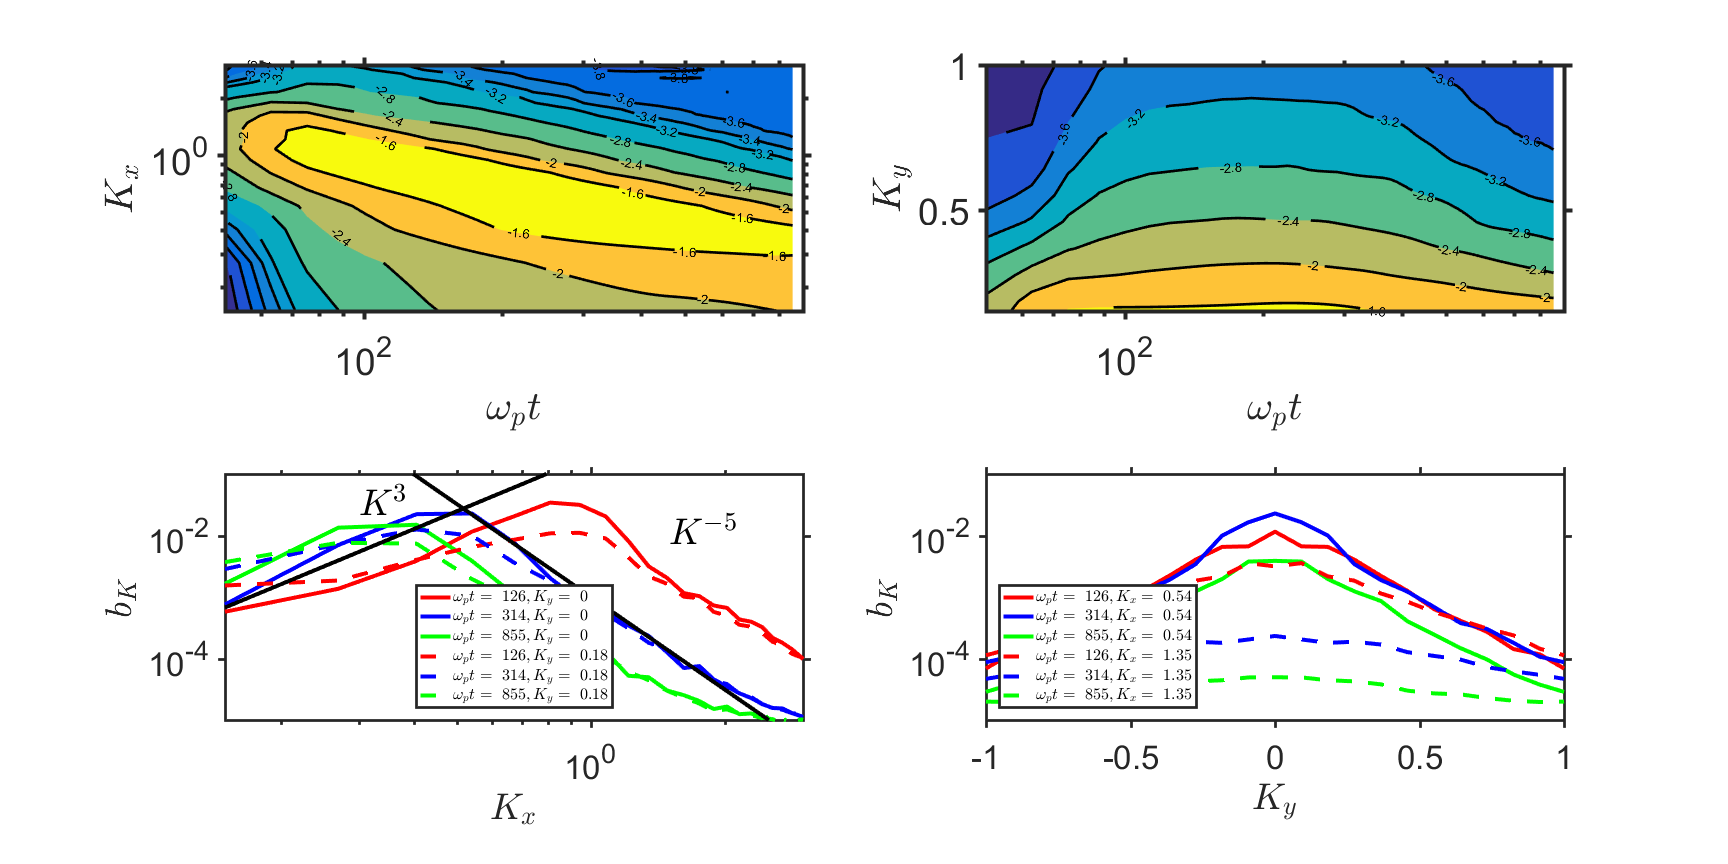
\includegraphics[width=1\linewidth]{part4/spectrA10_B0.png}
\captionstyle{normal}
\caption{Эволюция спектра турбулентности в двойном логарифмическом масштабе: (a)~линии уровня логарифма усредненных вдоль оси анизотропии амплитуд мод магнитного поля $|b_K|$; 
(b)~линии уровня логарифма усредненных поперек оси анизотропии амплитуд мод магнитного поля $|b_K|$; 
(c)~спектр $|b_K|$ магнитного поля поперек оси анизотропии при продольных волновых числах $K_\|=0$ (сплошная) и $K_\|=0.18$ (пунктир). 
(d)~спектр $|b_K|$ магнитного поля вдоль оси анизотропии при поперечных волновых числах $K_\perp=0.54$ (сплошная) и $K_\perp=1.35$ (пунктир) в моменты времени $\wpl t$, равные 126 (красный цвет), 314 (синий), 855 (зеленый). Внешнее магнитное поле отсутствует $b_{ext}=0$.
}
\label{ris:spectrA10_B0}
\end{figure}

Гармоники по-прежнему могут находиться на одной из 4 возможных стадий эволюции: экспоненциальный, степенной или сверхбысрый рост, а также осцилляционное затухание. Показатель степенного роста, который могут испытывать и нелинейно индуцированные сравнительно длинноволновые наклонные гармоники, по-прежнему оценивается от $1$ до $2$. Усреднение по аксиальному углу позволяет также выделить показатель усредненного затухания, который после добавления наклонных мод увеличивается и теперь оценивается от $-2$ до $-1.5$.  

В незамагниченной плазме продольная компонента турбулентного магнитного поля возникает исключительно вследствие нелинейной генерации. Во внешнем магнитном поле неустойчивая апериодическая мода обладает смешанной поляризацией (ни ТМ- ни ТЕ-), что существенно сближает и без того схожую и взаимосвязанную спектральную динамику поперечной и продольной компонент магнитного поля. Поэтому в последующих главах обсуждается спектр именно поперечной компоненты турбулентного магнитного поля. 


\subsection{Конкуренция вейбелевской и шланговой турбулентности и нелинейное взаимодействие мод в сравнительно слабом внешнем магнитном поле}
\label{part_spectr_b4}
Уже при $b_{ext}< b_{s\perp}$ значение линейного инкремента может оказаться существенно выше у наклонных мод апериодической неустойчивости, чем у поперечных мод, а значит, неучет наклонных мод становится невозможен. При сравнительно слабом внешнем магнитного поля $b_{ext}=0.4$~(рис. \ref{ris:spectrA10_B44}) инкремент поперечных мод все еще сравним с максимальным, но область неустойчивости как в поперечном, так и в продольном к оси анизотропии направлениях существенно уменьшается~\cite{Emelyanov2023_Radiophys,Moya2022}), а длинноволновая граница области неустойчивости становится отличной от нуля~(\ref{eq:border_perp_inst}). Помимо этого, апериодические неустойчивые моды теперь являются смешанными, то есть не являются ни ТЕ-, ни ТМ-модами. 



\begin{figure}[h]

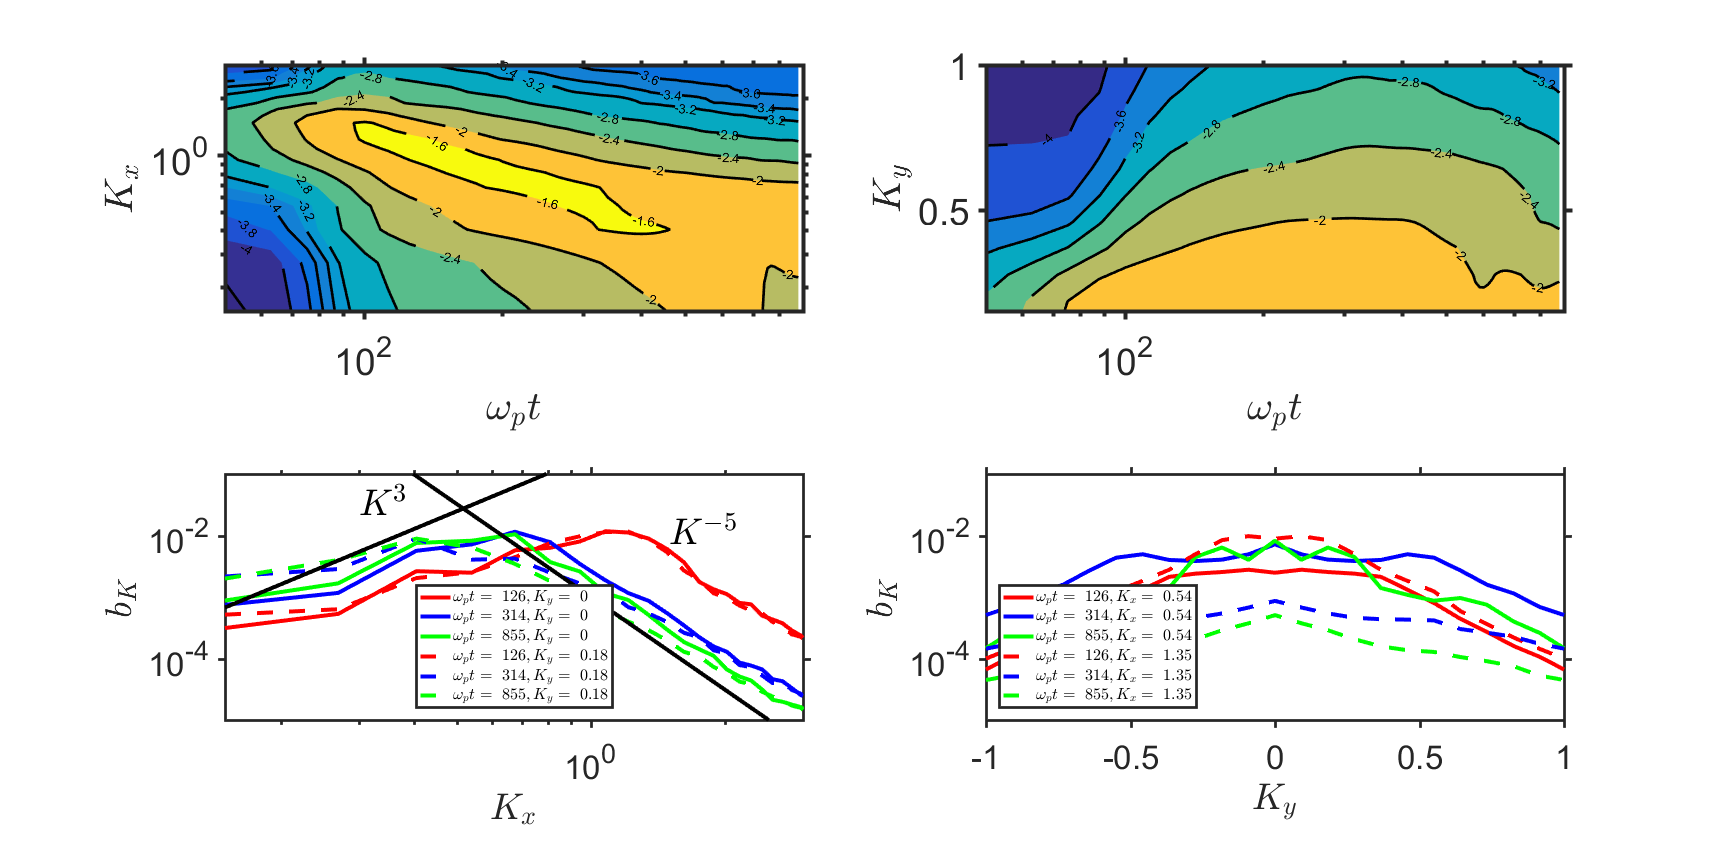
\includegraphics[width=1\linewidth]{part4/spectrA10_B44.png}
\captionstyle{normal}
\caption{Эволюция спектра турбулентности в двойном логарифмическом масштабе: (a)~линии уровня логарифма усредненных вдоль оси анизотропии амплитуд мод магнитного поля $|b_K|$; 
(b)~линии уровня логарифма усредненных поперек оси анизотропии амплитуд мод магнитного поля $|b_K|$; 
(c)~спектр $|b_K|$ магнитного поля поперек оси анизотропии при продольных волновых числах $K_\|=0$ (сплошная) и $K_\|=0.18$ (пунктир). 
(d)~спектр $|b_K|$ магнитного поля вдоль оси анизотропии при поперечных волновых числах $K_\perp=0.54$ (сплошная) и $K_\perp=1.35$ (пунктир) в моменты времени $\wpl t$, равные 126 (красный цвет), 314 (синий), 855 (зеленый). Внешнее магнитное поле $b_{ext}=0.44$.
}
\label{ris:spectrA10_B44}
\end{figure}



Из-за нелинейной генерации мод в длинноволновой области, спектр турбулентности вскоре после насыщения неустойчивости сравнительно быстро расширяется в эту область~(рис. \ref{ris:all_modes}b). Подобная сверхбыстрая генерация длинноволновых, линейно устойчивых мод, которые уже на временах, двукратно превосходящих время насыщения неустойчивости, становятся основными энергонесущими модами, отсутствует в квазилинейном приближении, что предопределяет отличную эволюцию спектра. В квазилинейных аксиально симметричных симуляциях наблюдаются лишь не затухающие колебания линейно неустойчивых мод, а смещение спектра за пределы области линейной неустойчивости отсутствует. Поэтому на временах уже двукратно превышающих момент насыщения неустойчивости спектр существенно не квазилинеен, что отражается на распределении частиц по скоростям~(ср. рис. \ref{ris:FR_A10_3d_B44} и рис. \ref{ris:FR_A10_3d_B44_QL}).



Тем не менее, многие черты квазилинейной эволюции спектральная динамика сохраняет: характерное волновое число по-прежнему смещается в длинноволновую область;  более коротковолновые моды, чем характерная в данный момент времени мода, осцилляционно затухают, а многие более длинноволновые, в том числе и нелинейно индуцированные при насыщении неустойчивости~--- нарастают по степенному закону. Затухание линейно неустойчивых гармоник замедляется в сравнении со случаем отсутствия внешнего магнитного поля и показатель их усредненного степенного затухания оценивается от $-1.3$ до $-0.8$. Показатели степенного нарастания основных энергонесущих гармоник по-прежнему лежат в промежутке от $1$ до $2$, в том числе и для некоторых нелинейно индуцированных длинноволновых мод. Исключением из обеих оценок являются длинноволновые, почти поперечные, нелинейно индуцированные моды $\left(K_x\lesssim0.6,K_y\lesssim0.1\right)$, показатели нарастания и затухания которых стремятся к нулю. Таким образом, хотя квазилинейное взаимодействие по-прежнему остается весьма существенным в присутствии внешнего магнитного поля, непосредственно вид наблюдаемого спектра турбулентного магнитного поля в значительной степени определяется прямым межмодовым нелинейным взаимодействием.


\subsection{Динамика спектра шланговой турбулентности и нелинейное взаимодействие мод в подавляющем поперечные моды внешнем магнитном поле}


Начиная с величины внешнего магнитного поля $b_{ext}=0.59$ анализ линейного дисперсионного соотношения предсказывает устойчивость поперечных мод ~(рис. \ref{ris:spectrA10_B65}). Оптимальный волновой вектор (волновой вектор с наибольшим линейным инкрементом) при $b_{ext}=0.59$ образует угол с осью анизотропии, приблизительно равный $77^\circ$, а область апериодической неустойчивости продолжает обужение как в продольном, так и в поперечном направлении. Топология области неустойчивости в трехмерном пространстве изменилась: ранее она состояла из одной связанной области, ограниченной квазитороидальной поверхностью, а теперь~--- из двух~(рис. \ref{ris:mode_coupling}). В ходе нелинейной динамики спектра, как и в работах~\cite{Camporeale2008,Hellinger2014}, наблюдается смещение его максимума в длинноволновую область и уменьшение отношения характерного поперечного волнового числа к продольному. На протяжении нелинейной эволюции существенны квазипоперечные  моды  $\left(K_\|<K_{\|opt}/2\right)$, сгенерированные в широком диапазоне волновых чисел за счет трехволнового взаимодействия линейно неустойчивых мод и нарастающие с инкрементами, близкими к удвоенному максимальному инкременту~(рис. \ref{ris:all_modes}c). К моменту насыщения неустойчивости амплитуда их магнитного поля в $2-4$ раза ниже амплитуды магнитного поля наиболее линейно неустойчивой моды, а на временах в $3-4$ раза более поздних они становятся основными энергонесущими модами. Моды с удвоенной к линейно неустойчивым модам продольной компонентой волнового вектора $\left(K_\|\approx2K_{\|opt}\right)$ генерируются за счет того же механизма в широком, сравнимом с областью линейной неустойчивости, диапазоне значений поперечной компоненты~(рис. \ref{ris:mode_coupling}b). Аналогично,  к моменту насыщения неустойчивости их амплитуда в $2-4$ раза ниже амплитуды наиболее линейно неустойчивых мод. В течение последующей эволюции часть из них может стать основными энергонесущими модами, но к концу симуляций наблюдается затухание удвоенных продольных мод. 


\begin{figure}[h!]

\includegraphics[width=1\linewidth]{part4/spectrA10_B65.png}
\captionstyle{normal}
\caption{Эволюция спектра турбулентности в двойном логарифмическом масштабе: (a)~линии уровня логарифма усредненных вдоль оси анизотропии амплитуд мод магнитного поля $|b_K|$; 
(b)~линии уровня логарифма усредненных поперек оси анизотропии амплитуд мод магнитного поля $|b_K|$; 
(c)~спектр $|b_K|$ магнитного поля поперек оси анизотропии при продольных волновых числах $K_\|=0$ (сплошная) и $K_\|=0.27$ (пунктир). 
(d)~спектр $|b_K|$ магнитного поля вдоль оси анизотропии при поперечных волновых числах $K_\perp=0.54$ (сплошная) и $K_\perp=1.35$ (пунктир) в моменты времени $\wpl t$, равные 126 (красный цвет), 314 (синий), 855 (зеленый). Внешнее безразмерное магнитное поле $b_{ext}=0.59$.
}
\label{ris:spectrA10_B65}
\end{figure}

По-прежнему выделяются 4 возможные стадии эволюции для гармоник. Линейно неустойчивые апериодические моды испытывают экспоненциальный рост в соответствии с дисперсионным соотношением. После насыщения своего роста каждая мода в отдельности осцилляционно затухает. При насыщении неустойчивости наблюдается сверхбыстрый рост поперечных и удвоенных продольных мод. 


%%В ходе дальнейшей нелинейной эволюции из-за деформации однородной компоненты функции распределения частиц по скоростям наблюдается примерно степенной рост сравнительно длинноволновых, изначально линейно устойчивых и не генерируемых нелинейно мод, с достаточно высокими показателями роста, близкими к 5. 
Область волновых чисел, в которой наблюдается степенной рост, можно грубо оценить: $K_{\|opt}\lesssim  K_\|\lesssim 2K_{\|opt}$, $0\lesssim K_\perp\lesssim 2K_{\perp opt}$. В работах~\cite{Camporeale2008,Hellinger2014} предполагается, что длинноволновое смещение спектра с уменьшением угла наклона между характерным волновым вектором и магнитным полем происходит квазилинейно, и предпринимаются попытки его объяснить на основе линейной теории. Важно, что скорость их степенного роста сравнима со скоростью экспоненциального роста линейно неустойчивых мод (а при внешнем поле $b_{ext}=0.71$ значительно превосходит), что кажется невероятным в контексте квазилинейного взаимодействия, так как наблюдаемое нарастание происходит при уже значительно изотропизованном распределении частиц по скоростям. 

%В будущем, чтобы проверить гипотезу о ключевой роли квазилинейного взаимодействия в наблюдаемом смещении основных энергонесущих мод, необходимо выяснить, неустойчиво ли среднее в пространстве распределение частиц по скоростям в обсуждаемом внешнем магнитном поле относительно мод, сравнительно быстрый степенной рост которых наблюдается при этом распределении. 

\subsection{Шланговая турбулентность и нелинейное взаимодействие мод в сильном внешнем магнитном поле}
\label{part_spectr_b78}

Оптимальный волновой вектор линейного роста апериодической неустойчивости при  $b_{ext}=0.78$ образует угол с осью анизотропии, приблизительно равный  $70^\circ$, а область неустойчивости крайне обужена около соответствующей моды. К моменту насыщения неустойчивости наблюдается нелинейная генерация не только поперечных и удвоенных продольных мод, но и гармоник с примерно утроенным и даже учетверенным оптимальным продольным волновым числом~(рис. \ref{ris:all_modes}d), что придает спектру вдоль оси анизотропии гребенчатую форму. Далее в ходе нелинейной эволюции поперечное волновое число наиболее энергонесущих мод уменьшается, а продольное~--- увеличивается. Вслед за спектральным смещением наиболее энергонесущих мод происходит пропорциональное смещение кратных индуцированных гармоник. Вследствие этого спектр сглаживается в продольном направлении, теряя гребенчатую форму. Подобный процесс происходил и при меньшем поле $b_{ext}=0.59$, но был менее заметен из-за скоротечности и более широкого спектра линейно неустойчивых мод.

\begin{figure}[h!]

\includegraphics[width=1\linewidth]{part4/spectrA10_B78.png}
\captionstyle{normal}
\caption{Эволюция спектра турбулентности в двойном логарифмическом масштабе: (a)~линии уровня логарифма усредненных вдоль оси анизотропии амплитуд мод магнитного поля $|b_K|$; 
(b)~линии уровня логарифма усредненных поперек оси анизотропии амплитуд мод магнитного поля $|b_K|$; 
(c)~спектр $|b_K|$ магнитного поля поперек оси анизотропии при продольных волновых числах $K_\|=0$ (сплошная) и $K_\|=0.37$ (пунктир). 
(d)~спектр $|b_K|$ магнитного поля вдоль оси анизотропии при поперечных волновых числах $K_\perp=0.54$ (сплошная) и $K_\perp=0.81$ (пунктир) в моменты времени $\wpl t$, равные 478 (красный цвет), 628 (синий), 855 (зеленый). Внешнее безразмерное магнитное поле $b_{ext}=0.71$.
}
\label{ris:spectrA10_B78}
\end{figure}

На протяжении линейной неустойчивости происходит экспоненциальный рост смешанных апериодических мод в соответствии с линейной теорией. При насыщении неустойчивости наблюдается нелинейная генерация квазипоперечных $\left(K_\|<K_{\|opt}/2\right)$, удвоенных $\left(K_\|\approx2K_{\|opt}\right)$ и утроенных $\left(K_\|\approx3K_{\|opt}\right)$ продольных гармоник, а также гармоник на коротковолновом хвосте области неустойчивости ($\left(K_\|\approx K_{\|opt},K_\perp\gtrsim2K_{\perp opt}\right)$). Квазипоперечные моды нарастают с инкрементами, близкими к удвоенным вследствие трехволнового взаимодействия. Подобно четырехволновой генерации утроенной моды в отсутствие внешнего магнитного поля, для нелинейной генерации гармоник на коротковолновом хвосте линейной области неустойчивости должны сложится три основные энергонесущие моды~(рис. \ref{ris:mode_coupling}b). Инкременты нелинейного роста удвоенных продольных мод оценить затруднительно из-за шумов, однако они оказывается существенно выше удвоенного линейного, что дает основание предполагать генерацию этих гармоник не только посредством простого сложения двух линейно неустойчивых мод, но и за счет нелинейных взаимодействий более высокого порядка. То же касается и генерации утроенной продольной моды (рис. \ref{ris:all_modes}d). К насыщению неустойчивости уровень квазипоперечных и удвоенных продольных мод примерно на порядок ниже основной энергонесущей моды, утроенной продольной~--- на два порядка, гармоник коротковолнового хвоста~--- примерно полтора порядка. В ходе нелинейного смещения максимума спектра в линейно устойчивую область происходит быстрая, нелинейная генерация мод, отдельные участки которой лучше аппроксимируются экспоненциальной функцией, а отдельные~--- степенной с показателем, достигающим $10$. 
\section{Условия применимости квазилинейного подхода к описанию шланговой турбулентности} 
низкое внешнее магнитное поле 
\chapter{Оформление различных элементов}\label{ch:ch1}

\section{Форматирование текста}\label{sec:ch1/sec1}

Мы можем сделать \textbf{жирный текст} и \textit{курсив}.

\section{Ссылки}\label{sec:ch1/sec2}

Сошлёмся на библиографию.
Одна ссылка: \cite[с.~54]{Sokolov}\cite[с.~36]{Gaidaenko}.
Две ссылки: \cite{Sokolov,Gaidaenko}.
Ссылка на собственные работы: \cite{vakbib1, confbib2}.
Много ссылок: %\cite[с.~54]{Lermontov,Management,Borozda} % такой «фокус»
%вызывает biblatex warning относительно опции sortcites, потому что неясно, к
%какому источнику относится уточнение о страницах, а bibtex об этой проблеме
%даже не предупреждает
\cite{Lermontov, Management, Borozda, Marketing, Constitution, FamilyCode,
    Gost.7.0.53, Razumovski, Lagkueva, Pokrovski, Methodology, Berestova,
    Kriger}%
\ifnumequal{\value{bibliosel}}{0}{% Примеры для bibtex8
    \cite{Sirotko, Lukina, Encyclopedia, Nasirova}%
}{% Примеры для biblatex через движок biber
    \cite{Sirotko2, Lukina2, Encyclopedia2, Nasirova2}%
}%
.
И~ещё немного ссылок:~\cite{Article,Book,Booklet,Conference,Inbook,Incollection,Manual,Mastersthesis,
    Misc,Phdthesis,Proceedings,Techreport,Unpublished}
% Следует обратить внимание, что пробел после запятой внутри \cite{}
% обрабатывается ожидаемо, а пробел перед запятой, может вызывать проблемы при
% обработке ссылок.
\cite{medvedev2006jelektronnye, CEAT:CEAT581, doi:10.1080/01932691.2010.513279,
    Gosele1999161,Li2007StressAnalysis, Shoji199895, test:eisner-sample,
    test:eisner-sample-shorted, AB_patent_Pomerantz_1968, iofis_patent1960}%
\ifnumequal{\value{bibliosel}}{0}{% Примеры для bibtex8
}{% Примеры для biblatex через движок biber
    \cite{patent2h, patent3h, patent2}%
}%
.

\ifnumequal{\value{bibliosel}}{0}{% Примеры для bibtex8
Попытка реализовать несколько ссылок на конкретные страницы
для \texttt{bibtex} реализации библиографии:
[\citenum{Sokolov}, с.~54; \citenum{Gaidaenko}, с.~36].
}{% Примеры для biblatex через движок biber
Несколько источников (мультицитата):
% Тут специально написано по-разному тире, для демонстрации, что
% применение специальных тире в настоящий момент в biblatex приводит к непоказу
% "с.".
\cites[vii--x, 5, 7]{Sokolov}[v"--~x, 25, 526]{Gaidaenko}[vii--x, 5, 7]{Techreport},
работает только в \texttt{biblatex} реализации библиографии.
}%

Ссылки на собственные работы:~\cite{vakbib1, confbib1}.

Сошлёмся на приложения: Приложение~\cref{app:A}, Приложение~\cref{app:B2}.

Сошлёмся на формулу: формула~\cref{eq:equation1}.

Сошлёмся на изображение: рисунок~\cref{fig:knuth}.

Стандартной практикой является добавление к ссылкам префикса, характеризующего тип элемента.
Это не является строгим требованием, но~позволяет лучше ориентироваться в документах большого размера.
Например, для ссылок на~рисунки используется префикс \textit{fig},
для ссылки на~таблицу "--- \textit{tab}.

В таблице \cref{tab:tab_pref} приложения~\cref{app:B4} приведён список рекомендуемых
к использованию стандартных префиксов.

В некоторых ситуациях возникает необходимость отойти от требований ГОСТ по оформлению ссылок на
литературу.
В таком случае можно воспользоваться дополнительными опциями пакета \verb+biblatex+.

Например, в ссылке на книгу~\cite{sobenin_kdv} использование опции \verb+maxnames=4+ позволяет
вывести имена всех четырёх авторов.
По ГОСТ имена последних трёх авторов опускаются.

Кроме того, часто возникают проблемы с транслитерованными инициалами. Некоторые буквы русского
алфавита по правилам транслитерации записываются двумя буквами латинского алфавита (ю-yu, ё-yo и
т.д.).
Такие инициалы \verb+biblatex+ будет сокращать до одной буквы, что неверно.
Поправить его работу можно использовав опцию \verb+giveninits=false+.
Пример использования этой опции можно видеть в ссылке~\cite{initials}.

\section{Формулы}\label{sec:ch1/sec3}

Благодаря пакету \textit{icomma}, \LaTeX~одинаково хорошо воспринимает
в~качестве десятичного разделителя и запятую (\(3,1415\)), и точку (\(3.1415\)).

\subsection{Ненумерованные одиночные формулы}\label{subsec:ch1/sec3/sub1}

Вот так может выглядеть формула, которую необходимо вставить в~строку
по~тексту: \(x \approx \sin x\) при \(x \to 0\).

А вот так выглядит ненумерованная отдельностоящая формула c подстрочными
и надстрочными индексами:
\[
    (x_1+x_2)^2 = x_1^2 + 2 x_1 x_2 + x_2^2
\]

Формула с неопределенным интегралом:
\[
    \int f(\alpha+x)=\sum\beta
\]

При использовании дробей формулы могут получаться очень высокие:
\[
    \frac{1}{\sqrt{2}+
        \displaystyle\frac{1}{\sqrt{2}+
            \displaystyle\frac{1}{\sqrt{2}+\cdots}}}
\]

В формулах можно использовать греческие буквы:
%Все \original... команды заранее, ради этого примера, определены в Dissertation\userstyles.tex
\[
    \alpha\beta\gamma\delta\originalepsilon\epsilon\zeta\eta\theta%
    \vartheta\iota\kappa\varkappa\lambda\mu\nu\xi\pi\varpi\rho\varrho%
    \sigma\varsigma\tau\upsilon\originalphi\phi\chi\psi\omega\Gamma\Delta%
    \Theta\Lambda\Xi\Pi\Sigma\Upsilon\Phi\Psi\Omega
\]
\[%https://texfaq.org/FAQ-boldgreek
    \boldsymbol{\alpha\beta\gamma\delta\originalepsilon\epsilon\zeta\eta%
        \theta\vartheta\iota\kappa\varkappa\lambda\mu\nu\xi\pi\varpi\rho%
        \varrho\sigma\varsigma\tau\upsilon\originalphi\phi\chi\psi\omega\Gamma%
        \Delta\Theta\Lambda\Xi\Pi\Sigma\Upsilon\Phi\Psi\Omega}
\]

Для добавления формул можно использовать пары \verb+$+\dots\verb+$+ и \verb+$$+\dots\verb+$$+,
но~они считаются устаревшими.
Лучше использовать их функциональные аналоги \verb+\(+\dots\verb+\)+ и \verb+\[+\dots\verb+\]+.

\subsection{Ненумерованные многострочные формулы}\label{subsec:ch1/sec3/sub2}

Вот так можно написать две формулы, не нумеруя их, чтобы знаки <<равно>> были
строго друг под другом:
\begin{align}
    f_W & =  \min \left( 1, \max \left( 0, \frac{W_{soil} / W_{max}}{W_{crit}} \right)  \right), \nonumber \\
    f_T & =  \min \left( 1, \max \left( 0, \frac{T_s / T_{melt}}{T_{crit}} \right)  \right), \nonumber
\end{align}

Выровнять систему ещё и по переменной \( x \) можно, используя окружение
\verb|alignedat| из пакета \verb|amsmath|. Вот так:
\[
|x| = \left\{
\begin{alignedat}{2}
     &   & x, \quad & \text{eсли } x\geqslant 0 \\
     & - & x, \quad & \text{eсли } x<0
\end{alignedat}
\right.
\]
Здесь первый амперсанд (в исходном \LaTeX\ описании формулы) означает
выравнивание по~левому краю, второй "--- по~\( x \), а~третий "--- по~слову
<<если>>. Команда \verb|\quad| делает большой горизонтальный пробел.

Ещё вариант:
\[
    |x|=
    \begin{cases}
        \phantom{-}x, \text{если } x \geqslant 0 \\
        -x, \text{если } x<0
    \end{cases}
\]

Кроме того, для  нумерованных формул \verb|alignedat| делает вертикальное
выравнивание номера формулы по центру формулы. Например, выравнивание
компонент вектора:
\begin{equation}
    \label{eq:2p3}
    \begin{alignedat}{2}
        {\mathbf{N}}_{o1n}^{(j)} = \,{\sin} \phi\,n\!\left(n+1\right)
        {\sin}\theta\,
        \pi_n\!\left({\cos} \theta\right)
        \frac{
        z_n^{(j)}\!\left( \rho \right)
        }{\rho}\,
         & {\boldsymbol{\hat{\mathrm e}}}_{r}\,+      \\
        +\,
        {\sin} \phi\,
        \tau_n\!\left({\cos} \theta\right)
        \frac{
        \left[\rho z_n^{(j)}\!\left( \rho \right)\right]^{\prime}
        }{\rho}\,
         & {\boldsymbol{\hat{\mathrm e}}}_{\theta}\,+ \\
        +\,
        {\cos} \phi\,
        \pi_n\!\left({\cos} \theta\right)
        \frac{
        \left[\rho z_n^{(j)}\!\left( \rho \right)\right]^{\prime}
        }{\rho}\,
         & {\boldsymbol{\hat{\mathrm e}}}_{\phi}\:.
    \end{alignedat}
\end{equation}

Ещё об отступах. Иногда для лучшей <<читаемости>> формул полезно
немного исправить стандартные интервалы \LaTeX\ с учётом логической
структуры самой формулы. Например в формуле~\cref{eq:2p3} добавлен
небольшой отступ \verb+\,+ между основными сомножителями, ниже
результат применения всех вариантов отступа:
\begin{align*}
    \backslash!             & \quad f(x) = x^2\! +3x\! +2         \\
    \mbox{по-умолчанию}     & \quad f(x) = x^2+3x+2               \\
    \backslash,             & \quad f(x) = x^2\, +3x\, +2         \\
    \backslash{:}           & \quad f(x) = x^2\: +3x\: +2         \\
    \backslash;             & \quad f(x) = x^2\; +3x\; +2         \\
    \backslash \mbox{space} & \quad f(x) = x^2\ +3x\ +2           \\
    \backslash \mbox{quad}  & \quad f(x) = x^2\quad +3x\quad +2   \\
    \backslash \mbox{qquad} & \quad f(x) = x^2\qquad +3x\qquad +2
\end{align*}

Можно использовать разные математические алфавиты:
\begin{align}
    \mathcal{ABCDEFGHIJKLMNOPQRSTUVWXYZ} \nonumber  \\
    \mathfrak{ABCDEFGHIJKLMNOPQRSTUVWXYZ} \nonumber \\
    \mathbb{ABCDEFGHIJKLMNOPQRSTUVWXYZ} \nonumber
\end{align}

Посмотрим на систему уравнений на примере аттрактора Лоренца:

\[
\left\{
\begin{array}{rl}
    \dot x = & \sigma (y-x)  \\
    \dot y = & x (r - z) - y \\
    \dot z = & xy - bz
\end{array}
\right.
\]

А для вёрстки матриц удобно использовать многоточия:
\[
    \left(
        \begin{array}{ccc}
            a_{11} & \ldots & a_{1n} \\
            \vdots & \ddots & \vdots \\
            a_{n1} & \ldots & a_{nn} \\
        \end{array}
    \right)
\]

\subsection{Нумерованные формулы}\label{subsec:ch1/sec3/sub3}

А вот так пишется нумерованная формула:
\begin{equation}
    \label{eq:equation1}
    e = \lim_{n \to \infty} \left( 1+\frac{1}{n} \right) ^n
\end{equation}

Нумерованных формул может быть несколько:
\begin{equation}
    \label{eq:equation2}
    \lim_{n \to \infty} \sum_{k=1}^n \frac{1}{k^2} = \frac{\pi^2}{6}
\end{equation}

Впоследствии на формулы~\cref{eq:equation1, eq:equation2} можно ссылаться.

Сделать так, чтобы номер формулы стоял напротив средней строки, можно,
используя окружение \verb|multlined| (пакет \verb|mathtools|) вместо
\verb|multline| внутри окружения \verb|equation|. Вот так:
\begin{equation} % \tag{S} % tag - вписывает свой текст
    \label{eq:equation3}
    \begin{multlined}
        1+ 2+3+4+5+6+7+\dots + \\
        + 50+51+52+53+54+55+56+57 + \dots + \\
        + 96+97+98+99+100=5050
    \end{multlined}
\end{equation}

Уравнения~\cref{eq:subeq_1,eq:subeq_2} демонстрируют возможности
окружения \verb|subequations| (пакет \verb|amsmath|).
\begin{subequations}
    \label{eq:subeq_1}
    \begin{gather}
        y = x^2 + 1 \label{eq:subeq_1-1} \\
        y = 2 x^2 - x + 1 \label{eq:subeq_1-2}
    \end{gather}
\end{subequations}
Ссылки на отдельные уравнения~\cref{eq:subeq_1-1,eq:subeq_1-2,eq:subeq_2-1}.
\begin{subequations}
    \label{eq:subeq_2}
    \begin{align}
        y & = x^3 + x^2 + x + 1 \label{eq:subeq_2-1} \\
        y & = x^2
    \end{align}
\end{subequations}

\subsection{Форматирование чисел и размерностей величин}\label{sec:units}

Числа форматируются при помощи команды \verb|\num|:
\num{5,3};
\num{2,3e8};
\num{12345,67890};
\num{2,6 d4};
\num{1+-2i};
\num{.3e45};
\num[exponent-base=2]{5 e64};
\num[exponent-base=2,exponent-to-prefix]{5 e64};
\num{1.654 x 2.34 x 3.430}
\num{1 2 x 3 / 4}.
Для написания последовательности чисел можно использовать команды \verb|\numlist| и \verb|\numrange|:
\numlist{10;30;50;70}; \numrange{10}{30}.
Значения углов можно форматировать при помощи команды \verb|\ang|:
\ang{2.67};
\ang{30,3};
\ang{-1;;};
\ang{;-2;};
\ang{;;-3};
\ang{300;10;1}.

Обратите внимание, что ГОСТ запрещает использование знака <<->> для обозначения отрицательных чисел
за исключением формул, таблиц и~рисунков.
Вместо него следует использовать слово <<минус>>.

Размерности можно записывать при помощи команд \verb|\si| и \verb|\SI|:
\si{\farad\squared\lumen\candela};
\si{\joule\per\mole\per\kelvin};
\si[per-mode = symbol-or-fraction]{\joule\per\mole\per\kelvin};
\si{\metre\per\second\squared};
\SI{0.10(5)}{\neper};
\SI{1.2-3i e5}{\joule\per\mole\per\kelvin};
\SIlist{1;2;3;4}{\tesla};
\SIrange{50}{100}{\volt}.
Список единиц измерений приведён в таблицах~\cref{tab:unit:base,
    tab:unit:derived,tab:unit:accepted,tab:unit:physical,tab:unit:other}.
Приставки единиц приведены в~таблице~\cref{tab:unit:prefix}.

С дополнительными опциями форматирования можно ознакомиться в~описании пакета \texttt{siunitx};
изменить или добавить единицы измерений можно в~файле \texttt{siunitx.cfg}.

\begin{table}
    \centering
    \captionsetup{justification=centering} % выравнивание подписи по-центру
    \caption{Основные величины СИ}\label{tab:unit:base}
    \begin{tabular}{llc}
        \toprule
        Название  & Команда          & Символ         \\
        \midrule
        Ампер     & \verb|\ampere|   & \si{\ampere}   \\
        Кандела   & \verb|\candela|  & \si{\candela}  \\
        Кельвин   & \verb|\kelvin|   & \si{\kelvin}   \\
        Килограмм & \verb|\kilogram| & \si{\kilogram} \\
        Метр      & \verb|\metre|    & \si{\metre}    \\
        Моль      & \verb|\mole|     & \si{\mole}     \\
        Секунда   & \verb|\second|   & \si{\second}   \\
        \bottomrule
    \end{tabular}
\end{table}

\begin{table}
    \small
    \centering
    \begin{threeparttable}% выравнивание подписи по границам таблицы
        \caption{Производные единицы СИ}\label{tab:unit:derived}
        \begin{tabular}{llc|llc}
            \toprule
            Название       & Команда               & Символ              & Название & Команда & Символ \\
            \midrule
            Беккерель      & \verb|\becquerel|     & \si{\becquerel}     &
            Ньютон         & \verb|\newton|        & \si{\newton}                                      \\
            Градус Цельсия & \verb|\degreeCelsius| & \si{\degreeCelsius} &
            Ом             & \verb|\ohm|           & \si{\ohm}                                         \\
            Кулон          & \verb|\coulomb|       & \si{\coulomb}       &
            Паскаль        & \verb|\pascal|        & \si{\pascal}                                      \\
            Фарад          & \verb|\farad|         & \si{\farad}         &
            Радиан         & \verb|\radian|        & \si{\radian}                                      \\
            Грей           & \verb|\gray|          & \si{\gray}          &
            Сименс         & \verb|\siemens|       & \si{\siemens}                                     \\
            Герц           & \verb|\hertz|         & \si{\hertz}         &
            Зиверт         & \verb|\sievert|       & \si{\sievert}                                     \\
            Генри          & \verb|\henry|         & \si{\henry}         &
            Стерадиан      & \verb|\steradian|     & \si{\steradian}                                   \\
            Джоуль         & \verb|\joule|         & \si{\joule}         &
            Тесла          & \verb|\tesla|         & \si{\tesla}                                       \\
            Катал          & \verb|\katal|         & \si{\katal}         &
            Вольт          & \verb|\volt|          & \si{\volt}                                        \\
            Люмен          & \verb|\lumen|         & \si{\lumen}         &
            Ватт           & \verb|\watt|          & \si{\watt}                                        \\
            Люкс           & \verb|\lux|           & \si{\lux}           &
            Вебер          & \verb|\weber|         & \si{\weber}                                       \\
            \bottomrule
        \end{tabular}
    \end{threeparttable}
\end{table}

\begin{table}
    \centering
    \begin{threeparttable}% выравнивание подписи по границам таблицы
        \caption{Внесистемные единицы}\label{tab:unit:accepted}

        \begin{tabular}{llc}
            \toprule
            Название        & Команда           & Символ          \\
            \midrule
            День            & \verb|\day|       & \si{\day}       \\
            Градус          & \verb|\degree|    & \si{\degree}    \\
            Гектар          & \verb|\hectare|   & \si{\hectare}   \\
            Час             & \verb|\hour|      & \si{\hour}      \\
            Литр            & \verb|\litre|     & \si{\litre}     \\
            Угловая минута  & \verb|\arcminute| & \si{\arcminute} \\
            Угловая секунда & \verb|\arcsecond| & \si{\arcsecond} \\ %
            Минута          & \verb|\minute|    & \si{\minute}    \\
            Тонна           & \verb|\tonne|     & \si{\tonne}     \\
            \bottomrule
        \end{tabular}
    \end{threeparttable}
\end{table}

\begin{table}
    \centering
    \captionsetup{justification=centering}
    \caption{Внесистемные единицы, получаемые из эксперимента}\label{tab:unit:physical}
    \begin{tabular}{llc}
        \toprule
        Название                & Команда                  & Символ                 \\
        \midrule
        Астрономическая единица & \verb|\astronomicalunit| & \si{\astronomicalunit} \\
        Атомная единица массы   & \verb|\atomicmassunit|   & \si{\atomicmassunit}   \\
        Боровский радиус        & \verb|\bohr|             & \si{\bohr}             \\
        Скорость света          & \verb|\clight|           & \si{\clight}           \\
        Дальтон                 & \verb|\dalton|           & \si{\dalton}           \\
        Масса электрона         & \verb|\electronmass|     & \si{\electronmass}     \\
        Электрон Вольт          & \verb|\electronvolt|     & \si{\electronvolt}     \\
        Элементарный заряд      & \verb|\elementarycharge| & \si{\elementarycharge} \\
        Энергия Хартри          & \verb|\hartree|          & \si{\hartree}          \\
        Постоянная Планка       & \verb|\planckbar|        & \si{\planckbar}        \\
        \bottomrule
    \end{tabular}
\end{table}

\begin{table}
    \centering
    \begin{threeparttable}% выравнивание подписи по границам таблицы
        \caption{Другие внесистемные единицы}\label{tab:unit:other}
        \begin{tabular}{llc}
            \toprule
            Название                  & Команда              & Символ             \\
            \midrule
            Ангстрем                  & \verb|\angstrom|     & \si{\angstrom}     \\
            Бар                       & \verb|\bar|          & \si{\bar}          \\
            Барн                      & \verb|\barn|         & \si{\barn}         \\
            Бел                       & \verb|\bel|          & \si{\bel}          \\
            Децибел                   & \verb|\decibel|      & \si{\decibel}      \\
            Узел                      & \verb|\knot|         & \si{\knot}         \\
            Миллиметр ртутного столба & \verb|\mmHg|         & \si{\mmHg}         \\
            Морская миля              & \verb|\nauticalmile| & \si{\nauticalmile} \\
            Непер                     & \verb|\neper|        & \si{\neper}        \\
            \bottomrule
        \end{tabular}
    \end{threeparttable}
\end{table}

\begin{table}
    \small
    \centering
    \begin{threeparttable}% выравнивание подписи по границам таблицы
        \caption{Приставки СИ}\label{tab:unit:prefix}
        \begin{tabular}{llcc|llcc}
            \toprule
            Приставка & Команда       & Символ      & Степень      &
            Приставка & Команда       & Символ      & Степень        \\
            \midrule
            Иокто     & \verb|\yocto| & \si{\yocto} & \textminus24 &
            Дека      & \verb|\deca|  & \si{\deca}  & 1              \\
            Зепто     & \verb|\zepto| & \si{\zepto} & \textminus21 &
            Гекто     & \verb|\hecto| & \si{\hecto} & 2              \\
            Атто      & \verb|\atto|  & \si{\atto}  & \textminus18 &
            Кило      & \verb|\kilo|  & \si{\kilo}  & 3              \\
            Фемто     & \verb|\femto| & \si{\femto} & \textminus15 &
            Мега      & \verb|\mega|  & \si{\mega}  & 6              \\
            Пико      & \verb|\pico|  & \si{\pico}  & \textminus12 &
            Гига      & \verb|\giga|  & \si{\giga}  & 9              \\
            Нано      & \verb|\nano|  & \si{\nano}  & \textminus9  &
            Терра     & \verb|\tera|  & \si{\tera}  & 12             \\
            Микро     & \verb|\micro| & \si{\micro} & \textminus6  &
            Пета      & \verb|\peta|  & \si{\peta}  & 15             \\
            Милли     & \verb|\milli| & \si{\milli} & \textminus3  &
            Екса      & \verb|\exa|   & \si{\exa}   & 18             \\
            Санти     & \verb|\centi| & \si{\centi} & \textminus2  &
            Зетта     & \verb|\zetta| & \si{\zetta} & 21             \\
            Деци      & \verb|\deci|  & \si{\deci}  & \textminus1  &
            Иотта     & \verb|\yotta| & \si{\yotta} & 24             \\
            \bottomrule
        \end{tabular}
    \end{threeparttable}
\end{table}

\subsection{Заголовки с формулами: \texorpdfstring{\(a^2 + b^2 = c^2\)}{%
        a\texttwosuperior\ + b\texttwosuperior\ = c\texttwosuperior},
    \texorpdfstring{\(\left\vert\textrm{{Im}}\Sigma\left(
            \protect\varepsilon\right)\right\vert\approx const\)}{|ImΣ (ε)| ≈ const},
    \texorpdfstring{\(\sigma_{xx}^{(1)}\)}{σ\_\{xx\}\textasciicircum\{(1)\}}
}\label{subsec:with_math}

Пакет \texttt{hyperref} берёт текст для закладок в pdf-файле из~аргументов
команд типа \verb|\section|, которые могут содержать математические формулы,
а~также изменения цвета текста или шрифта, которые не отображаются в~закладках.
Чтобы использование формул в заголовках не вызывало в~логе компиляции появление
предупреждений типа <<\texttt{Token not allowed in~a~PDF string
    (Unicode):(hyperref) removing...}>>, следует использовать конструкцию
\verb|\texorpdfstring{}{}|, где в~первых фигурных скобках указывается
формула, а~во~вторых "--- запись формулы для закладок.

\section{Рецензирование текста}\label{sec:markup}

В шаблоне для диссертации и автореферата заданы команды рецензирования.
Они видны при компиляции шаблона в режиме черновика или при установке
соответствующей настройки (\verb+showmarkup+) в~файле \verb+common/setup.tex+.

Команда \verb+\todo+ отмечает текст красным цветом.
\todo{Например, так.}

Команда \verb+\note+ позволяет выбрать цвет текста.
\note{Чёрный, } \note[red]{красный, } \note[green]{зелёный, }
\note[blue]{синий.} \note[orange]{Обратите внимание на ширину и расстановку
    формирующихся пробелов, в~результате приведённой записи (зависит также
    от~применяемого компилятора).}

Окружение \verb+commentbox+ также позволяет выбрать цвет.

\begin{commentbox}[red]
    Красный текст.

    Несколько параграфов красного текста.
\end{commentbox}

\begin{commentbox}[blue]
    Синяя формула.

    \begin{equation}
        \alpha + \beta = \gamma
    \end{equation}
\end{commentbox}

\verb+commentbox+ позволяет закомментировать участок кода в~режиме чистовика.
Чтобы убрать кусок кода для всех режимов, можно использовать окружение
\verb+comment+.

\begin{comment}
Этот текст всегда скрыт.
\end{comment}

\section{Работа со списком сокращений и~условных обозначений}\label{sec:acronyms}

С помощью пакета \texttt{nomencl} можно создавать удобный сортированный список
сокращений и условных обозначений во время написания текста. Вызов
\verb+\nomenclature+ добавляет нужный символ или сокращение с~описанием
в~список, который затем печатается вызовом \verb+\printnomenclature+
в~соответствующем разделе.
Для того, чтобы эти операции прошли, потребуется дополнительный вызов
\verb+makeindex -s nomencl.ist -o %.nls %.nlo+ в~командной строке, где вместо
\verb+%+ следует подставить имя главного файла проекта (\verb+dissertation+
для этого шаблона).
Затем потребуется один или два дополнительных вызова компилятора проекта.
\begin{equation}
    \omega = c k,
\end{equation}
где \( \omega \) "--- частота света, \( c \) "--- скорость света, \( k \) "---
модуль волнового вектора.
\nomenclature{\(\omega\)}{частота света\nomrefeq}
\nomenclature{\(c\)}{скорость света\nomrefpage}
\nomenclature{\(k\)}{модуль волнового вектора\nomrefeqpage}
Использование
\begin{verbatim}
\nomenclature{\(\omega\)}{частота света\nomrefeq}
\nomenclature{\(c\)}{скорость света\nomrefpage}
\nomenclature{\(k\)}{модуль волнового вектора\nomrefeqpage}
\end{verbatim}
после уравнения добавит в список условных обозначений три записи.
Ссылки \verb+\nomrefeq+ на последнее уравнение, \verb+\nomrefpage+ "--- на
страницу, \verb+\nomrefeqpage+ "--- сразу на~последнее уравнение и~на~страницу,
можно опускать и~не~использовать.

Группировкой и сортировкой пунктов в списке можно управлять с~помощью указания
дополнительных аргументов к команде \verb+nomenclature+.
Например, при вызове
\begin{verbatim}
\nomenclature[03]{\( \hbar \)}{постоянная Планка}
\nomenclature[01]{\( G \)}{гравитационная постоянная}
\end{verbatim}
\( G \) будет стоять в списке выше, чем \( \hbar \).
Для корректных вертикальных отступов между строками в описании лучше
не~использовать многострочные формулы в~списке обозначений.

\nomenclature{%
    \( \begin{rcases}
        a_n \\
        b_n
    \end{rcases} \)%
}{коэффициенты разложения Ми в дальнем поле соответствующие электрическим и
    магнитным мультиполям}
\nomenclature[a\( e \)]{\( {\boldsymbol{\hat{\mathrm e}}} \)}{единичный вектор}
\nomenclature{\( E_0 \)}{амплитуда падающего поля}
\nomenclature{\( j \)}{тип функции Бесселя}
\nomenclature{\( k \)}{волновой вектор падающей волны}
\nomenclature{%
    \( \begin{rcases}
        a_n \\
        b_n
    \end{rcases} \)%
}{и снова коэффициенты разложения Ми в дальнем поле соответствующие
    электрическим и магнитным мультиполям. Добавлено много текста, так что
    описание группы условных обозначений значительно превысило высоту этой
    группы...}
\nomenclature{\( L \)}{общее число слоёв}
\nomenclature{\( l \)}{номер слоя внутри стратифицированной сферы}
\nomenclature{\( \lambda \)}{длина волны электромагнитного излучения в вакууме}
\nomenclature{\( n \)}{порядок мультиполя}
\nomenclature{%
    \( \begin{rcases}
        {\mathbf{N}}_{e1n}^{(j)} & {\mathbf{N}}_{o1n}^{(j)} \\
        {\mathbf{M}_{o1n}^{(j)}} & {\mathbf{M}_{e1n}^{(j)}}
    \end{rcases} \)%
}{сферические векторные гармоники}
\nomenclature{\( \mu \)}{магнитная проницаемость в вакууме}
\nomenclature{\( r, \theta, \phi \)}{полярные координаты}
\nomenclature{\( \omega \)}{частота падающей волны}

С помощью \verb+nomenclature+ можно включать в~список сокращения,
не~используя их~в~тексте.
% запись сокращения в список происходит командой \nomenclature,
% а не употреблением самого сокращения
\nomenclature{FEM}{finite element method, метод конечных элементов}
\nomenclature{FIT}{finite integration technique, метод конечных интегралов}
\nomenclature{FMM}{fast multipole method, быстрый метод многополюсника}
\nomenclature{FVTD}{finite volume time-domain, метод конечных объёмов
    во~временной области}
\nomenclature{MLFMA}{multilevel fast multipole algorithm, многоуровневый
    быстрый алгоритм многополюсника}
\nomenclature{BEM}{boundary element method, метод граничных элементов}
\nomenclature{CST MWS}{Computer Simulation Technology Microwave Studio
    программа для компьютерного моделирования уравнен Максвелла}
\nomenclature{DDA}{discrete dipole approximation, приближение дискретиных
    диполей}
\nomenclature{FDFD}{finite difference frequency domain, метод конечных
    разностей в~частотной области}
\nomenclature{FDTD}{finite difference time domain, метод конечных разностей
    во~временной области}
\nomenclature{MoM}{method of moments, метод моментов}
\nomenclature{MSTM}{multiple sphere T-Matrix, метод Т-матриц для множества
    сфер}
\nomenclature{PSTD}{pseudospectral time domain method, псевдоспектральный метод
    во~временной области}
\nomenclature{TLM}{transmission line matrix method, метод матриц линий передач}

\FloatBarrier
 
\include{Dissertation/conclusion}      % Заключение

\include{Dissertation/references}      % Список литературы


\setcounter{totalchapter}{\value{chapter}} % Подсчёт количества глав

%%% Настройки для приложений
\appendix
% Оформление заголовков приложений ближе к ГОСТ:
\setlength{\midchapskip}{20pt}
\renewcommand*{\afterchapternum}{\par\nobreak\vskip \midchapskip}
\renewcommand\thechapter{\Asbuk{chapter}} % Чтобы приложения русскими буквами нумеровались



\setcounter{totalappendix}{\value{chapter}} % Подсчёт количества приложений

\end{document}
